\clearpage

%%%%%%%%%%% DIST %%%%%%%%%%%%%%%%%%
\begin{figure}
  \centering

  \begin{overpic}[clip, rviewport=0 0 1 1,width=0.4\textwidth]{dedx/dist_350_v0_c0_x13_y3}
    \put(16,85){(a)}
  \end{overpic}
  \begin{overpic}[clip, rviewport=0 0 1 1,width=0.4\textwidth]{dedx/dist_350_v0_c1_x13_y3}
    \put(16,85){(b)}
  \end{overpic}

  \vspace{0.5cm}
  
  \begin{overpic}[clip, rviewport=0 0 1 1,width=0.4\textwidth]{dedx/dist_350_v1_c0_x29_y5}
    \put(16,85){(c)}
  \end{overpic}
  \begin{overpic}[clip, rviewport=0 0 1 1,width=0.4\textwidth]{dedx/dist_350_v1_c1_x29_y5}
    \put(16,85){(d)}
  \end{overpic}
  
  \caption{Examples of the fitted \dedx distributions from the 350 \GeVc dataset.
    On the top, the distributions of the (a) negatively and (b) positively charged
    tracks are shown for one phase space bin of the RST subset. On the bottom,
    the distributions of the (c) negatively and (d) positively charged
    tracks are shown for a different phase space bin of the WST subset.
    The values of the $\langle\pp\rangle$ and $\langle\pT\rangle$ for
    each phase space bin is indicated on the top of each plot.
    The black dots show the observed number of tracks, while the colored
    distributions are the results of the \dedx fit or each particle type. 
    On the bottom of each plot, we show the residual of the fit, defined
    as the difference between the observed and the expected number of tracks
    from the result of the fit, divided by the uncertainty of the observed number.}
  \label{fig:hadron:dedx:fit:dist350}
\end{figure}



%%%%%%%%%% CHI SQ %%%%%%%%%%%%%%
\begin{figure}
  \centering

  \begin{overpic}[clip, rviewport=0 0 1 0.945,width=0.4\textwidth]{dedx/chisq_350_v0}
    \put(18,58){(a)}
  \end{overpic}
  \begin{overpic}[clip, rviewport=0 0 1 0.945,width=0.4\textwidth]{dedx/chisq_350_v0}
    \put(18,58){(b)}
  \end{overpic}

  \caption{\redchisq of the \dedx fit for the 350 \GeVc data set.
    The RST and WST are shown in (a) and (b), respectively.}
  \label{fig:hadron:dedx:fit:chi350}
\end{figure}

%%%%%%%%%% CAL %%%%%%%%%%%%%%
\begin{figure}[!ht]
  \centering

  \begin{overpic}[clip, rviewport=0 0 1 0.94,width=0.49\textwidth]{dedx/model_158_v1_m0}
    \put(18,58){(a)}
  \end{overpic}
  \begin{overpic}[clip, rviewport=0 0 1 0.94,width=0.49\textwidth]{dedx/model_158_v1_m1}
    \put(18,58){(b)}
  \end{overpic}

  \begin{overpic}[clip, rviewport=0 0 1 0.94,width=0.49\textwidth]{dedx/model_158_v1_m2}
    \put(18,58){(c)}
  \end{overpic}
  \begin{overpic}[clip, rviewport=0 0 1 0.94,width=0.49\textwidth]{dedx/model_158_v1_m3}
    \put(18,58){(d)}
  \end{overpic}

  \begin{overpic}[clip, rviewport=0 0 1 0.94,width=0.49\textwidth]{dedx/model_158_v1_m4}
    \put(18,58){(e)}
  \end{overpic}
  \begin{overpic}[clip, rviewport=0 0 1 0.94,width=0.49\textwidth]{dedx/model_158_v1_m5}
    \put(18,58){(f)}
  \end{overpic}

  \caption{Calibration constants obtained from the \dedx fit of the WST and 158 \GeVc data set.}
  \label{fig:hadron:dedx:fit:cal158w}
\end{figure}

%%%%%%%%%% CAL %%%%%%%%%%%%%%
\begin{figure}[!ht]
  \centering

  \begin{overpic}[clip, rviewport=0 0 1 0.94,width=0.49\textwidth]{dedx/model_350_v0_m0}
    \put(18,58){(a)}
  \end{overpic}
  \begin{overpic}[clip, rviewport=0 0 1 0.94,width=0.49\textwidth]{dedx/model_350_v0_m1}
    \put(18,58){(b)}
  \end{overpic}

  \begin{overpic}[clip, rviewport=0 0 1 0.94,width=0.49\textwidth]{dedx/model_350_v0_m2}
    \put(18,58){(c)}
  \end{overpic}
  \begin{overpic}[clip, rviewport=0 0 1 0.94,width=0.49\textwidth]{dedx/model_350_v0_m3}
    \put(18,58){(d)}
  \end{overpic}

  \begin{overpic}[clip, rviewport=0 0 1 0.94,width=0.49\textwidth]{dedx/model_350_v0_m4}
    \put(18,58){(e)}
  \end{overpic}
  \begin{overpic}[clip, rviewport=0 0 1 0.94,width=0.49\textwidth]{dedx/model_350_v0_m5}
    \put(18,58){(f)}
  \end{overpic}

  \caption{Calibration constants obtained from the \dedx fit of the RST and 350 \GeVc data set.}
  \label{fig:hadron:dedx:fit:cal350r}
\end{figure}


%%%%%%%%%% CAL %%%%%%%%%%%%%%
\begin{figure}[!ht]
  \centering

  \begin{overpic}[clip, rviewport=0 0 1 0.94,width=0.49\textwidth]{dedx/model_350_v1_m0}
    \put(18,58){(a)}
  \end{overpic}
  \begin{overpic}[clip, rviewport=0 0 1 0.94,width=0.49\textwidth]{dedx/model_350_v1_m1}
    \put(18,58){(b)}
  \end{overpic}

  \begin{overpic}[clip, rviewport=0 0 1 0.94,width=0.49\textwidth]{dedx/model_350_v1_m2}
    \put(18,58){(c)}
  \end{overpic}
  \begin{overpic}[clip, rviewport=0 0 1 0.94,width=0.49\textwidth]{dedx/model_350_v1_m3}
    \put(18,58){(d)}
  \end{overpic}

  \begin{overpic}[clip, rviewport=0 0 1 0.94,width=0.49\textwidth]{dedx/model_350_v1_m4}
    \put(18,58){(e)}
  \end{overpic}
  \begin{overpic}[clip, rviewport=0 0 1 0.94,width=0.49\textwidth]{dedx/model_350_v1_m5}
    \put(18,58){(f)}
  \end{overpic}

  \caption{Calibration constants obtained from the \dedx fit of the WST and 350 \GeVc data set.}
  \label{fig:hadron:dedx:fit:cal350w}
\end{figure}

\clearpage

%%%%%%%%%% SHAPE %%%%%%%%%%%%%%
\begin{figure}[!ht]
  \centering

  \begin{overpic}[clip, rviewport=0 0 1 0.94,width=0.49\textwidth]{dedx/model_158_v1_m6}
    \put(18,58){(a)}
  \end{overpic}
  \begin{overpic}[clip, rviewport=0 0 1 0.94,width=0.49\textwidth]{dedx/model_158_v1_m7}
    \put(18,58){(b)}
  \end{overpic}

  \begin{overpic}[clip, rviewport=0 0 1 0.94,width=0.49\textwidth]{dedx/model_158_v1_m9}
    \put(18,58){(c)}
  \end{overpic}
  \begin{overpic}[clip, rviewport=0 0 1 0.94,width=0.49\textwidth]{dedx/model_158_v1_m10}
    \put(18,58){(d)}
  \end{overpic}

  \caption{Shape parameters obtained from the \dedx fit of the WST and 158 \GeVc data set.}
  \label{fig:hadron:dedx:fit:shape158w}
\end{figure}

%%%%%%%%%% SHAPE %%%%%%%%%%%%%%
\begin{figure}[!ht]
  \centering

  \begin{overpic}[clip, rviewport=0 0 1 0.94,width=0.49\textwidth]{dedx/model_350_v0_m6}
    \put(18,58){(a)}
  \end{overpic}
  \begin{overpic}[clip, rviewport=0 0 1 0.94,width=0.49\textwidth]{dedx/model_350_v0_m7}
    \put(18,58){(b)}
  \end{overpic}

  \begin{overpic}[clip, rviewport=0 0 1 0.94,width=0.49\textwidth]{dedx/model_350_v0_m9}
    \put(18,58){(c)}
  \end{overpic}
  \begin{overpic}[clip, rviewport=0 0 1 0.94,width=0.49\textwidth]{dedx/model_350_v0_m10}
    \put(18,58){(d)}
  \end{overpic}

  \caption{Shape parameters obtained from the \dedx fit of the RST and 350 \GeVc data set.}
  \label{fig:hadron:dedx:fit:shape350r}
\end{figure}

%%%%%%%%%% SHAPE %%%%%%%%%%%%%%
\begin{figure}[!ht]
  \centering

  \begin{overpic}[clip, rviewport=0 0 1 0.94,width=0.49\textwidth]{dedx/model_350_v1_m6}
    \put(18,58){(a)}
  \end{overpic}
  \begin{overpic}[clip, rviewport=0 0 1 0.94,width=0.49\textwidth]{dedx/model_350_v1_m7}
    \put(18,58){(b)}
  \end{overpic}

  \begin{overpic}[clip, rviewport=0 0 1 0.94,width=0.49\textwidth]{dedx/model_350_v1_m9}
    \put(18,58){(c)}
  \end{overpic}
  \begin{overpic}[clip, rviewport=0 0 1 0.94,width=0.49\textwidth]{dedx/model_350_v1_m10}
    \put(18,58){(d)}
  \end{overpic}

  \caption{Shape parameters obtained from the \dedx fit of the WST and 350 \GeVc data set.}
  \label{fig:hadron:dedx:fit:shape350w}
\end{figure}


\clearpage



%%%%%%%%%% FRACTIONS %%%%%%%%%%%%%%
\begin{figure}
  \centering

  \begin{overpic}[clip, rviewport=0 0.125 1 0.94,width=0.45\textwidth]{dedx/fraction_158_fl0_v1_c0_p0}
    \put(18,49){(a)}
  \end{overpic}
  \begin{overpic}[clip, rviewport=0 0.125 1 0.94,width=0.45\textwidth]{dedx/fraction_158_fl0_v1_c1_p0}
    \put(18,49){(b)}
  \end{overpic}

  \begin{overpic}[clip, rviewport=0 0.125 1 0.94,width=0.45\textwidth]{dedx/fraction_158_fl0_v1_c0_p1}
    \put(18,49){(c)}
  \end{overpic}
  \begin{overpic}[clip, rviewport=0 0.125 1 0.94,width=0.45\textwidth]{dedx/fraction_158_fl0_v1_c1_p1}
    \put(18,49){(d)}
  \end{overpic}

   \begin{overpic}[clip, rviewport=0 0.125 1 0.94,width=0.45\textwidth]{dedx/fraction_158_fl0_v1_c0_p2}
    \put(18,49){(e)}
  \end{overpic}
  \begin{overpic}[clip, rviewport=0 0.125 1 0.94,width=0.45\textwidth]{dedx/fraction_158_fl0_v1_c1_p2}
    \put(18,49){(f)}
  \end{overpic}

   \begin{overpic}[clip, rviewport=0 0.125 1 0.94,width=0.45\textwidth]{dedx/fraction_158_fl0_v1_c0_p3}
    \put(18,49){(g)}
  \end{overpic}
  \begin{overpic}[clip, rviewport=0 0.125 1 0.94,width=0.45\textwidth]{dedx/fraction_158_fl0_v1_c1_p3}
    \put(18,49){(h)}
  \end{overpic}

   \begin{overpic}[clip, rviewport=0 0 1 0.94,width=0.45\textwidth]{dedx/fraction_158_fl0_v1_c0_p4}
    \put(18,58){(i)}
  \end{overpic}
  \begin{overpic}[clip, rviewport=0 0 1 0.94,width=0.45\textwidth]{dedx/fraction_158_fl0_v1_c1_p4}
    \put(18,58){(j)}
  \end{overpic}
  
  \caption{Particle fractions obtained from the \dedx fit of the WST and 158 \GeVc data set.}
  \label{fig:hadron:dedx:fit:frac158w}
\end{figure}


%%%%%%%%%% FRACTIONS %%%%%%%%%%%%%%
\begin{figure}
  \centering

  \begin{overpic}[clip, rviewport=0 0.125 1 0.94,width=0.45\textwidth]{dedx/fraction_350_fl0_v0_c0_p0}
    \put(18,49){(a)}
  \end{overpic}
  \begin{overpic}[clip, rviewport=0 0.125 1 0.94,width=0.45\textwidth]{dedx/fraction_350_fl0_v0_c1_p0}
    \put(18,49){(b)}
  \end{overpic}

  \begin{overpic}[clip, rviewport=0 0.125 1 0.94,width=0.45\textwidth]{dedx/fraction_350_fl0_v0_c0_p1}
    \put(18,49){(c)}
  \end{overpic}
  \begin{overpic}[clip, rviewport=0 0.125 1 0.94,width=0.45\textwidth]{dedx/fraction_350_fl0_v0_c1_p1}
    \put(18,49){(d)}
  \end{overpic}

   \begin{overpic}[clip, rviewport=0 0.125 1 0.94,width=0.45\textwidth]{dedx/fraction_350_fl0_v0_c0_p2}
    \put(18,49){(e)}
  \end{overpic}
  \begin{overpic}[clip, rviewport=0 0.125 1 0.94,width=0.45\textwidth]{dedx/fraction_350_fl0_v0_c1_p2}
    \put(18,49){(f)}
  \end{overpic}

   \begin{overpic}[clip, rviewport=0 0.125 1 0.94,width=0.45\textwidth]{dedx/fraction_350_fl0_v0_c0_p3}
    \put(18,49){(g)}
  \end{overpic}
  \begin{overpic}[clip, rviewport=0 0.125 1 0.94,width=0.45\textwidth]{dedx/fraction_350_fl0_v0_c1_p3}
    \put(18,49){(h)}
  \end{overpic}

   \begin{overpic}[clip, rviewport=0 0 1 0.94,width=0.45\textwidth]{dedx/fraction_350_fl0_v0_c0_p4}
    \put(18,58){(i)}
  \end{overpic}
  \begin{overpic}[clip, rviewport=0 0 1 0.94,width=0.45\textwidth]{dedx/fraction_350_fl0_v0_c1_p4}
    \put(18,58){(j)}
  \end{overpic}
  
  \caption{Particle fractions obtained from the \dedx fit of the RST and 350 \GeVc data set.}
  \label{fig:hadron:dedx:fit:frac350r}
\end{figure}


%%%%%%%%%% FRACTIONS %%%%%%%%%%%%%%
\begin{figure}
  \centering

  \begin{overpic}[clip, rviewport=0 0.125 1 0.94,width=0.45\textwidth]{dedx/fraction_350_fl0_v1_c0_p0}
    \put(18,49){(a)}
  \end{overpic}
  \begin{overpic}[clip, rviewport=0 0.125 1 0.94,width=0.45\textwidth]{dedx/fraction_350_fl0_v1_c1_p0}
    \put(18,49){(b)}
  \end{overpic}

  \begin{overpic}[clip, rviewport=0 0.125 1 0.94,width=0.45\textwidth]{dedx/fraction_350_fl0_v1_c0_p1}
    \put(18,49){(c)}
  \end{overpic}
  \begin{overpic}[clip, rviewport=0 0.125 1 0.94,width=0.45\textwidth]{dedx/fraction_350_fl0_v1_c1_p1}
    \put(18,49){(d)}
  \end{overpic}

   \begin{overpic}[clip, rviewport=0 0.125 1 0.94,width=0.45\textwidth]{dedx/fraction_350_fl0_v1_c0_p2}
    \put(18,49){(e)}
  \end{overpic}
  \begin{overpic}[clip, rviewport=0 0.125 1 0.94,width=0.45\textwidth]{dedx/fraction_350_fl0_v1_c1_p2}
    \put(18,49){(f)}
  \end{overpic}

   \begin{overpic}[clip, rviewport=0 0.125 1 0.94,width=0.45\textwidth]{dedx/fraction_350_fl0_v1_c0_p3}
    \put(18,49){(g)}
  \end{overpic}
  \begin{overpic}[clip, rviewport=0 0.125 1 0.94,width=0.45\textwidth]{dedx/fraction_350_fl0_v1_c1_p3}
    \put(18,49){(h)}
  \end{overpic}

   \begin{overpic}[clip, rviewport=0 0 1 0.94,width=0.45\textwidth]{dedx/fraction_350_fl0_v1_c0_p4}
    \put(18,58){(i)}
  \end{overpic}
  \begin{overpic}[clip, rviewport=0 0 1 0.94,width=0.45\textwidth]{dedx/fraction_350_fl0_v1_c1_p4}
    \put(18,58){(j)}
  \end{overpic}
  
  \caption{Particle fractions obtained from the \dedx fit of the WST and 350 \GeVc data set.}
  \label{fig:hadron:dedx:fit:frac350w}
\end{figure}

\clearpage

%%%%%%%%%% FAKE REL SIG %%%%%%%%%%%%%%
\begin{figure}[!ht]
  \centering
  
  \begin{overpic}[clip, rviewport=0 0.145 1 0.94,width=0.45\textwidth]{dedx/fake_rel_sig_158_fl0_v1_c0_p1}
    \put(18,48){(a)}
  \end{overpic}
  \begin{overpic}[clip, rviewport=0 0.145 1 0.94,width=0.45\textwidth]{dedx/fake_rel_sig_158_fl0_v1_c1_p1}
    \put(18,48){(b)}
  \end{overpic}

  \begin{overpic}[clip, rviewport=0 0.145 1 0.94,width=0.45\textwidth]{dedx/fake_rel_sig_158_fl0_v1_c0_p2}
    \put(18,48){(c)}
  \end{overpic}
  \begin{overpic}[clip, rviewport=0 0.145 1 0.94,width=0.45\textwidth]{dedx/fake_rel_sig_158_fl0_v1_c1_p2}
    \put(18,48){(d)}
  \end{overpic}

  \begin{overpic}[clip, rviewport=0 0 1 0.94,width=0.45\textwidth]{dedx/fake_rel_sig_158_fl0_v1_c0_p3}
    \put(18,58){(e)}
  \end{overpic}
  \begin{overpic}[clip, rviewport=0 0 1 0.94,width=0.45\textwidth]{dedx/fake_rel_sig_158_fl0_v1_c1_p3}
    \put(18,58){(f)}
  \end{overpic}
  
  \caption{Relative standard deviation ($\sigma_r$, see the definition in the text) of the particle fractions obtained with the SDEs for the WST and 158 \GeVc case. The $\pi^+$ case is shown in (a), $\pi^-$ in (b), K$^+$ in (c), K$^-$ in (d), p$^+$ in (e) and p$^-$ in (f).}
  \label{fig:hadron:dedx:fit:fake:relsig158w}
\end{figure}

%%%%%%%%%% FAKE REL SIG %%%%%%%%%%%%%%
\begin{figure}[!ht]
  \centering
  
  \begin{overpic}[clip, rviewport=0 0.145 1 0.94,width=0.45\textwidth]{dedx/fake_rel_sig_350_fl0_v0_c0_p1}
    \put(18,48){(a)}
  \end{overpic}
  \begin{overpic}[clip, rviewport=0 0.145 1 0.94,width=0.45\textwidth]{dedx/fake_rel_sig_350_fl0_v0_c1_p1}
    \put(18,48){(b)}
  \end{overpic}

  \begin{overpic}[clip, rviewport=0 0.145 1 0.94,width=0.45\textwidth]{dedx/fake_rel_sig_350_fl0_v0_c0_p2}
    \put(18,48){(c)}
  \end{overpic}
  \begin{overpic}[clip, rviewport=0 0.145 1 0.94,width=0.45\textwidth]{dedx/fake_rel_sig_350_fl0_v0_c1_p2}
    \put(18,48){(d)}
  \end{overpic}

  \begin{overpic}[clip, rviewport=0 0 1 0.94,width=0.45\textwidth]{dedx/fake_rel_sig_350_fl0_v0_c0_p3}
    \put(18,58){(e)}
  \end{overpic}
  \begin{overpic}[clip, rviewport=0 0 1 0.94,width=0.45\textwidth]{dedx/fake_rel_sig_350_fl0_v0_c1_p3}
    \put(18,58){(f)}
  \end{overpic}
  
  \caption{Relative standard deviation ($\sigma_r$, see the definition in the text) of the particle fractions obtained with the SDEs for the RST and 350 \GeVc case. The $\pi^+$ case is shown in (a), $\pi^-$ in (b), K$^+$ in (c), K$^-$ in (d), p$^+$ in (e) and p$^-$ in (f).}
  \label{fig:hadron:dedx:fit:fake:relsig350r}
\end{figure}


%%%%%%%%%% FAKE REL SIG %%%%%%%%%%%%%%
\begin{figure}[!ht]
  \centering
  
  \begin{overpic}[clip, rviewport=0 0.145 1 0.94,width=0.45\textwidth]{dedx/fake_rel_sig_350_fl0_v1_c0_p1}
    \put(18,48){(a)}
  \end{overpic}
  \begin{overpic}[clip, rviewport=0 0.145 1 0.94,width=0.45\textwidth]{dedx/fake_rel_sig_350_fl0_v1_c1_p1}
    \put(18,48){(b)}
  \end{overpic}

  \begin{overpic}[clip, rviewport=0 0.145 1 0.94,width=0.45\textwidth]{dedx/fake_rel_sig_350_fl0_v1_c0_p2}
    \put(18,48){(c)}
  \end{overpic}
  \begin{overpic}[clip, rviewport=0 0.145 1 0.94,width=0.45\textwidth]{dedx/fake_rel_sig_350_fl0_v1_c1_p2}
    \put(18,48){(d)}
  \end{overpic}

  \begin{overpic}[clip, rviewport=0 0 1 0.94,width=0.45\textwidth]{dedx/fake_rel_sig_350_fl0_v1_c0_p3}
    \put(18,58){(e)}
  \end{overpic}
  \begin{overpic}[clip, rviewport=0 0 1 0.94,width=0.45\textwidth]{dedx/fake_rel_sig_350_fl0_v1_c1_p3}
    \put(18,58){(f)}
  \end{overpic}
  
  \caption{Relative standard deviation ($\sigma_r$, see the definition in the text) of the particle fractions obtained with the SDEs for the WST and 350 \GeVc case. The $\pi^+$ case is shown in (a), $\pi^-$ in (b), K$^+$ in (c), K$^-$ in (d), p$^+$ in (e) and p$^-$ in (f).}
  \label{fig:hadron:dedx:fit:fake:relsig350w}
\end{figure}


%%%%%%%%%% FAKE REL DEV %%%%%%%%%%%%%%
\begin{figure}[!ht]
  \centering
  
  \begin{overpic}[clip, rviewport=0 0.145 1 0.94,width=0.45\textwidth]{dedx/fake_rel_dev_158_fl0_v1_c0_p1}
    \put(18,48){(a)}
  \end{overpic}
  \begin{overpic}[clip, rviewport=0 0.145 1 0.94,width=0.45\textwidth]{dedx/fake_rel_dev_158_fl0_v1_c1_p1}
    \put(18,48){(b)}
  \end{overpic}

  \begin{overpic}[clip, rviewport=0 0.145 1 0.94,width=0.45\textwidth]{dedx/fake_rel_dev_158_fl0_v1_c0_p2}
    \put(18,48){(c)}
  \end{overpic}
  \begin{overpic}[clip, rviewport=0 0.145 1 0.94,width=0.45\textwidth]{dedx/fake_rel_dev_158_fl0_v1_c1_p2}
    \put(18,48){(d)}
  \end{overpic}

  \begin{overpic}[clip, rviewport=0 0 1 0.94,width=0.45\textwidth]{dedx/fake_rel_dev_158_fl0_v1_c0_p3}
    \put(18,58){(e)}
  \end{overpic}
  \begin{overpic}[clip, rviewport=0 0 1 0.94,width=0.45\textwidth]{dedx/fake_rel_dev_158_fl0_v1_c1_p3}
    \put(18,58){(f)}
  \end{overpic}
  
  \caption{Average relative bias ($\delta_r$, see the definition in the text) of the particle fractions obtained with the SDEs for the WST and 158 \GeVc case. The $\pi^+$ case is shown in (a), $\pi^-$ in (b), K$^+$ in (c), K$^-$ in (d), p$^+$ in (e) and p$^-$ in (f).}
  \label{fig:hadron:dedx:fit:fake:reldev158w}
\end{figure}

%%%%%%%%%% FAKE REL DEV %%%%%%%%%%%%%%
\begin{figure}[!ht]
  \centering
  
  \begin{overpic}[clip, rviewport=0 0.145 1 0.94,width=0.45\textwidth]{dedx/fake_rel_dev_350_fl0_v0_c0_p1}
    \put(18,48){(a)}
  \end{overpic}
  \begin{overpic}[clip, rviewport=0 0.145 1 0.94,width=0.45\textwidth]{dedx/fake_rel_dev_350_fl0_v0_c1_p1}
    \put(18,48){(b)}
  \end{overpic}

  \begin{overpic}[clip, rviewport=0 0.145 1 0.94,width=0.45\textwidth]{dedx/fake_rel_dev_350_fl0_v0_c0_p2}
    \put(18,48){(c)}
  \end{overpic}
  \begin{overpic}[clip, rviewport=0 0.145 1 0.94,width=0.45\textwidth]{dedx/fake_rel_dev_350_fl0_v0_c1_p2}
    \put(18,48){(d)}
  \end{overpic}

  \begin{overpic}[clip, rviewport=0 0 1 0.94,width=0.45\textwidth]{dedx/fake_rel_dev_350_fl0_v0_c0_p3}
    \put(18,58){(e)}
  \end{overpic}
  \begin{overpic}[clip, rviewport=0 0 1 0.94,width=0.45\textwidth]{dedx/fake_rel_dev_350_fl0_v0_c1_p3}
    \put(18,58){(f)}
  \end{overpic}
  
  \caption{Average relative bias ($\delta_r$, see the definition in the text) of the particle fractions obtained with the SDEs for the RST and 350 \GeVc case. The $\pi^+$ case is shown in (a), $\pi^-$ in (b), K$^+$ in (c), K$^-$ in (d), p$^+$ in (e) and p$^-$ in (f).}
  \label{fig:hadron:dedx:fit:fake:reldev350r}
\end{figure}

%%%%%%%%%% FAKE REL DEV %%%%%%%%%%%%%%
\begin{figure}[!ht]
  \centering
  
  \begin{overpic}[clip, rviewport=0 0.145 1 0.94,width=0.45\textwidth]{dedx/fake_rel_dev_350_fl0_v1_c0_p1}
    \put(18,48){(a)}
  \end{overpic}
  \begin{overpic}[clip, rviewport=0 0.145 1 0.94,width=0.45\textwidth]{dedx/fake_rel_dev_350_fl0_v1_c1_p1}
    \put(18,48){(b)}
  \end{overpic}

  \begin{overpic}[clip, rviewport=0 0.145 1 0.94,width=0.45\textwidth]{dedx/fake_rel_dev_350_fl0_v1_c0_p2}
    \put(18,48){(c)}
  \end{overpic}
  \begin{overpic}[clip, rviewport=0 0.145 1 0.94,width=0.45\textwidth]{dedx/fake_rel_dev_350_fl0_v1_c1_p2}
    \put(18,48){(d)}
  \end{overpic}

  \begin{overpic}[clip, rviewport=0 0 1 0.94,width=0.45\textwidth]{dedx/fake_rel_dev_350_fl0_v1_c0_p3}
    \put(18,58){(e)}
  \end{overpic}
  \begin{overpic}[clip, rviewport=0 0 1 0.94,width=0.45\textwidth]{dedx/fake_rel_dev_350_fl0_v1_c1_p3}
    \put(18,58){(f)}
  \end{overpic}
  
  \caption{Average relative bias ($\delta_r$, see the definition in the text) of the particle fractions obtained with the SDEs for the RST and 350 \GeVc case. The $\pi^+$ case is shown in (a), $\pi^-$ in (b), K$^+$ in (c), K$^-$ in (d), p$^+$ in (e) and p$^-$ in (f).}
  \label{fig:hadron:dedx:fit:fake:reldev350r}
\end{figure}


\clearpage


%%%%%%%%%% COR %%%%%%%%%%%%%%
\begin{figure}[!ht]
  \centering

  \begin{overpic}[clip, rviewport=0 0.145 1 0.94,width=0.45\textwidth]{dedx/cor_158_v1_c0_p1}
    \put(18,48){(a)}
  \end{overpic}
  \begin{overpic}[clip, rviewport=0 0.145 1 0.94,width=0.45\textwidth]{dedx/cor_158_v1_c0_p1}
    \put(18,48){(b)}
  \end{overpic}

  \begin{overpic}[clip, rviewport=0 0.145 1 0.94,width=0.45\textwidth]{dedx/cor_158_v1_c0_p2}
    \put(18,48){(c)}
  \end{overpic}
  \begin{overpic}[clip, rviewport=0 0.145 1 0.94,width=0.45\textwidth]{dedx/cor_158_v1_c0_p2}
    \put(18,48){(d)}
  \end{overpic}

  \begin{overpic}[clip, rviewport=0 0 1 0.94,width=0.45\textwidth]{dedx/cor_158_v1_c0_p3}
    \put(18,58){(e)}
  \end{overpic}
  \begin{overpic}[clip, rviewport=0 0 1 0.94,width=0.45\textwidth]{dedx/cor_158_v1_c0_p3}
    \put(18,58){(f)}
  \end{overpic}
  
  \caption{Correction factors ($c$, see the definition in the text) for the WST and 158 \GeVc case. The $\pi^+$ case is shown in (a), $\pi^-$ in (b), K$^+$ in (c), K$^-$ in (d), p$^+$ in (e) and p$^-$ in (f).}
  \label{fig:hadron:dedx:fit:fake:cor158w}
\end{figure}

%%%%%%%%%% COR %%%%%%%%%%%%%%
\begin{figure}[!ht]
  \centering

  \begin{overpic}[clip, rviewport=0 0.145 1 0.94,width=0.45\textwidth]{dedx/cor_350_v0_c0_p1}
    \put(18,48){(a)}
  \end{overpic}
  \begin{overpic}[clip, rviewport=0 0.145 1 0.94,width=0.45\textwidth]{dedx/cor_350_v0_c0_p1}
    \put(18,48){(b)}
  \end{overpic}

  \begin{overpic}[clip, rviewport=0 0.145 1 0.94,width=0.45\textwidth]{dedx/cor_350_v0_c0_p2}
    \put(18,48){(c)}
  \end{overpic}
  \begin{overpic}[clip, rviewport=0 0.145 1 0.94,width=0.45\textwidth]{dedx/cor_350_v0_c0_p2}
    \put(18,48){(d)}
  \end{overpic}

  \begin{overpic}[clip, rviewport=0 0 1 0.94,width=0.45\textwidth]{dedx/cor_350_v0_c0_p3}
    \put(18,58){(e)}
  \end{overpic}
  \begin{overpic}[clip, rviewport=0 0 1 0.94,width=0.45\textwidth]{dedx/cor_350_v0_c0_p3}
    \put(18,58){(f)}
  \end{overpic}
  
  \caption{Correction factors ($c$, see the definition in the text) for the RST and 350 \GeVc case. The $\pi^+$ case is shown in (a), $\pi^-$ in (b), K$^+$ in (c), K$^-$ in (d), p$^+$ in (e) and p$^-$ in (f).}
  \label{fig:hadron:dedx:fit:fake:cor350r}
\end{figure}

%%%%%%%%%% COR %%%%%%%%%%%%%%
\begin{figure}[!ht]
  \centering

  \begin{overpic}[clip, rviewport=0 0.145 1 0.94,width=0.45\textwidth]{dedx/cor_350_v1_c0_p1}
    \put(18,48){(a)}
  \end{overpic}
  \begin{overpic}[clip, rviewport=0 0.145 1 0.94,width=0.45\textwidth]{dedx/cor_350_v1_c0_p1}
    \put(18,48){(b)}
  \end{overpic}

  \begin{overpic}[clip, rviewport=0 0.145 1 0.94,width=0.45\textwidth]{dedx/cor_350_v1_c0_p2}
    \put(18,48){(c)}
  \end{overpic}
  \begin{overpic}[clip, rviewport=0 0.145 1 0.94,width=0.45\textwidth]{dedx/cor_350_v1_c0_p2}
    \put(18,48){(d)}
  \end{overpic}

  \begin{overpic}[clip, rviewport=0 0 1 0.94,width=0.45\textwidth]{dedx/cor_350_v1_c0_p3}
    \put(18,58){(e)}
  \end{overpic}
  \begin{overpic}[clip, rviewport=0 0 1 0.94,width=0.45\textwidth]{dedx/cor_350_v1_c0_p3}
    \put(18,58){(f)}
  \end{overpic}
  
  \caption{Correction factors ($c$, see the definition in the text) for the RST and 350 \GeVc case. The $\pi^+$ case is shown in (a), $\pi^-$ in (b), K$^+$ in (c), K$^-$ in (d), p$^+$ in (e) and p$^-$ in (f).}
  \label{fig:hadron:dedx:fit:fake:cor350w}
\end{figure}



\clearpage

%%%%%%%%%% FRACTION %%%%%%%%%%%%%%

\begin{figure}
  \centering
  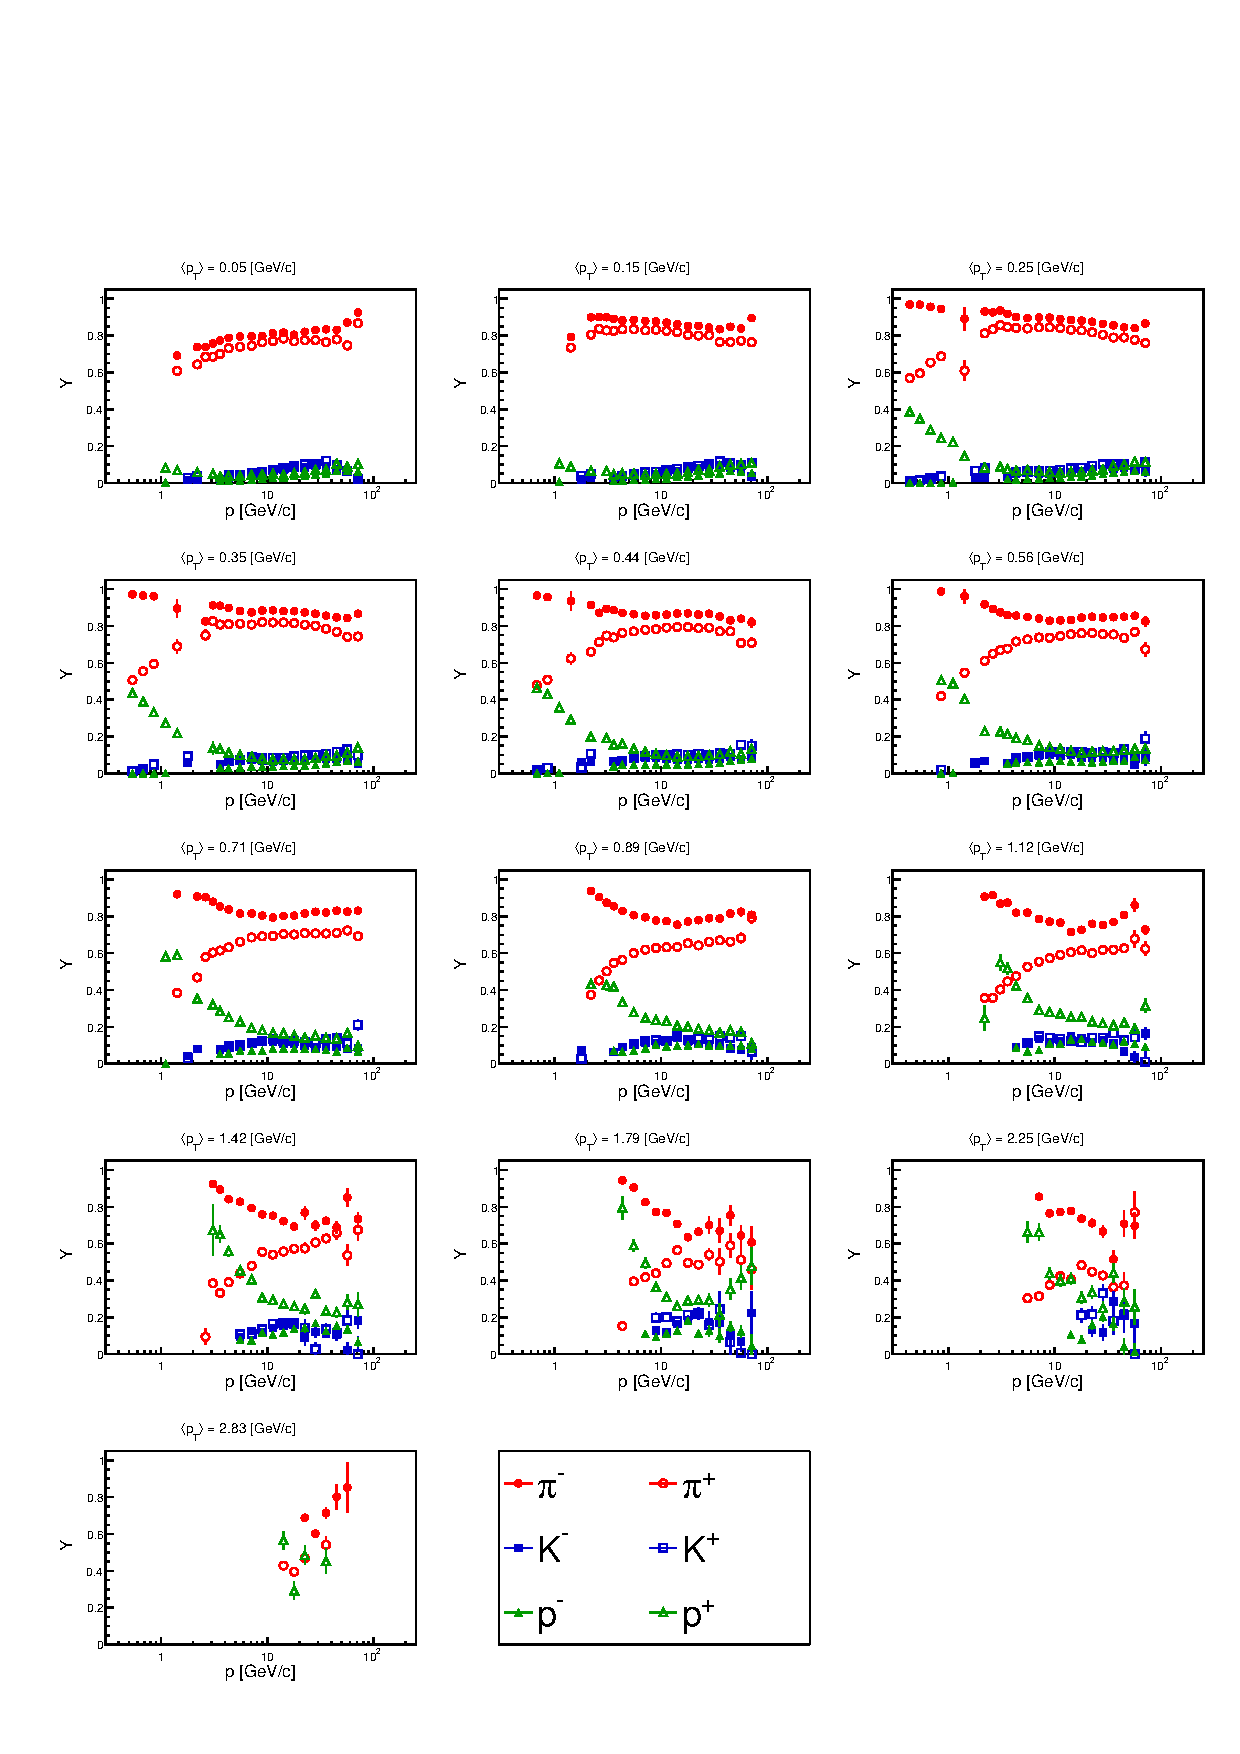
\includegraphics[clip, rviewport=0 0 1 1,width=1.00\textwidth]{dedx/fraction_pt_158_fl2_v1}
  \caption{Particle fractions obtained from the \dedx fit of the WST and 158 \GeVc dataset, with target inserted.}
  \label{fig:hadron:dedx:fit:final158w}
\end{figure}

\begin{figure}
  \centering
  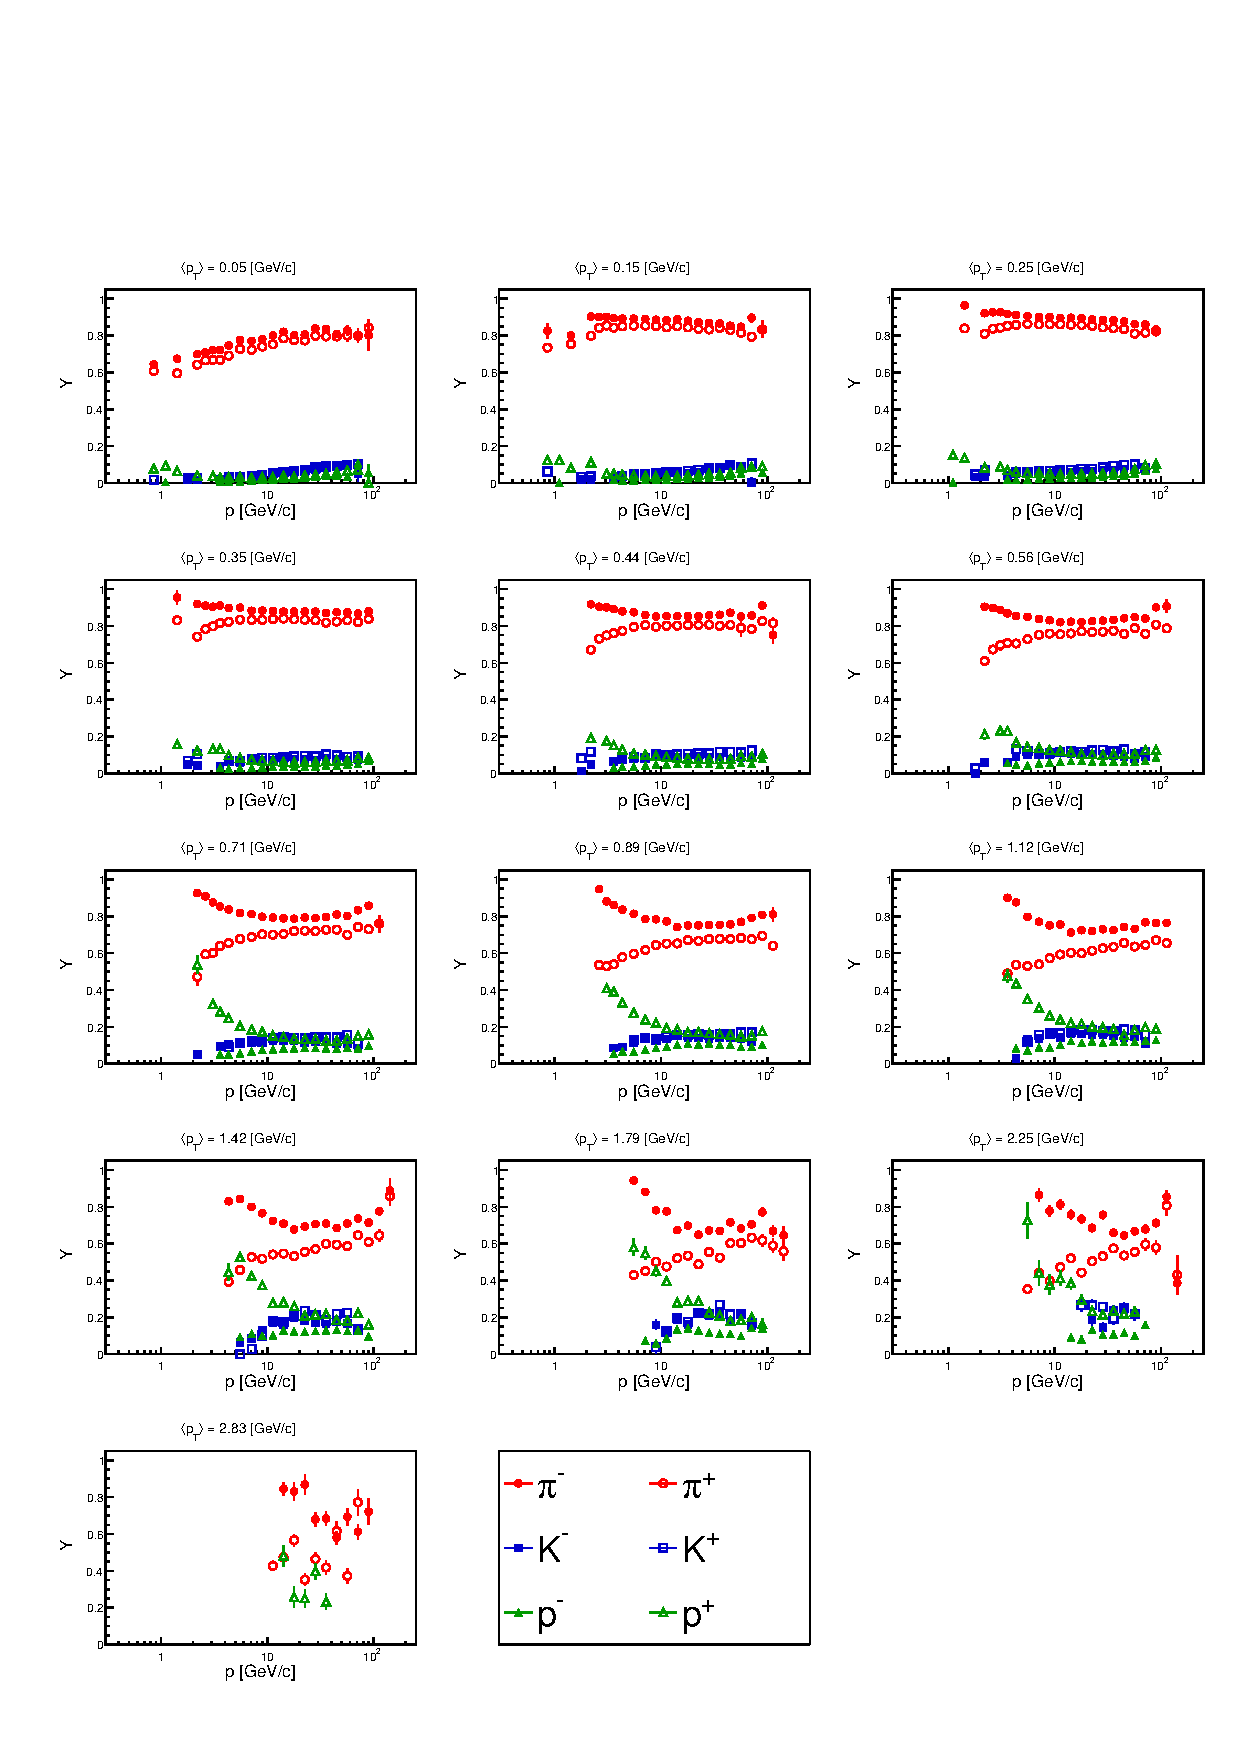
\includegraphics[clip, rviewport=0 0 1 1,width=1.00\textwidth]{dedx/fraction_pt_350_fl2_v0}
  \caption{Particle fractions obtained from the \dedx fit of the RST and 350 \GeVc dataset, with target inserted.}
  \label{fig:hadron:dedx:fit:final350r}
\end{figure}

\begin{figure}
  \centering
  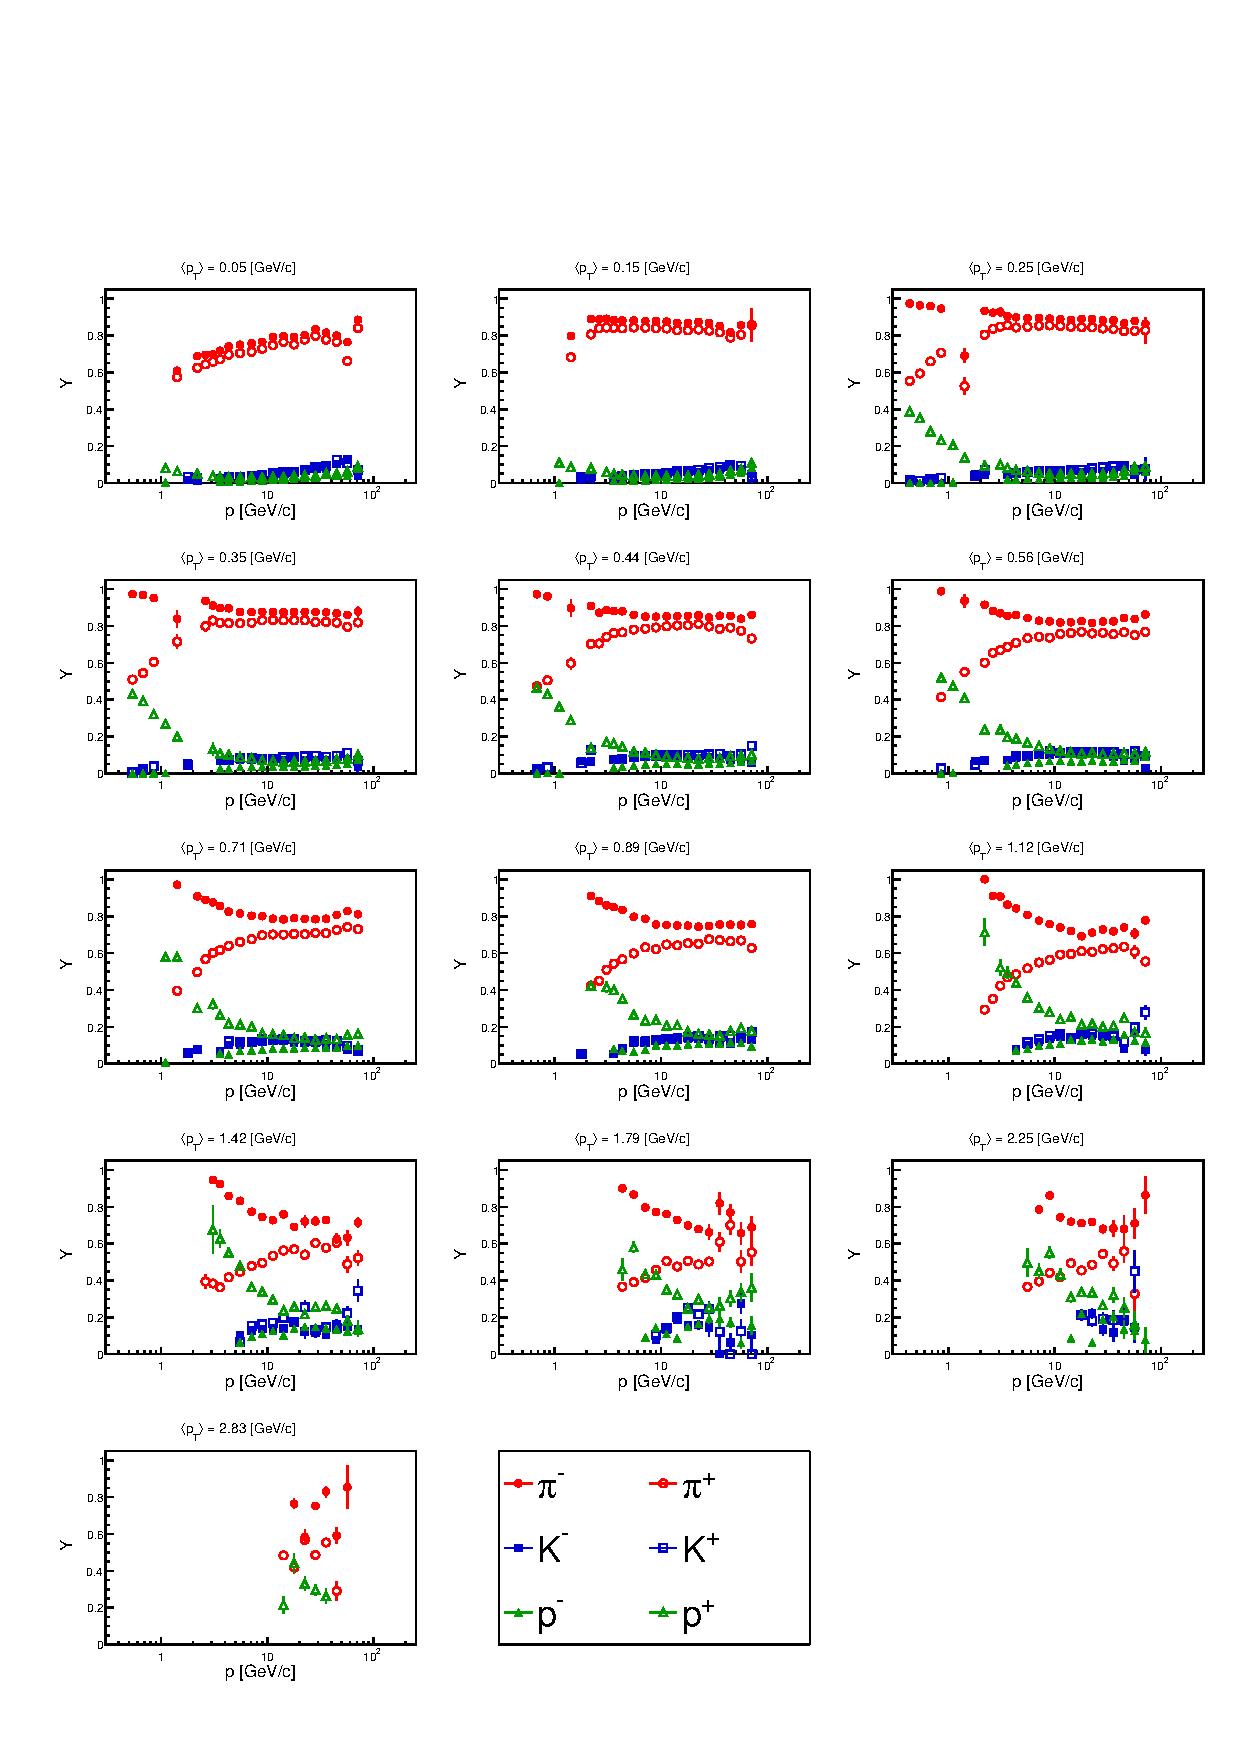
\includegraphics[clip, rviewport=0 0 1 1,width=1.00\textwidth]{dedx/fraction_pt_350_fl2_v1}
  \caption{Particle fractions obtained from the \dedx fit of the WST and 350 \GeVc dataset, with target inserted.}
  \label{fig:hadron:dedx:fit:final350w}
\end{figure}

%%%%%%%%%% FRACTION OUT%%%%%%%%%%%%%%
\begin{figure}
  \centering
  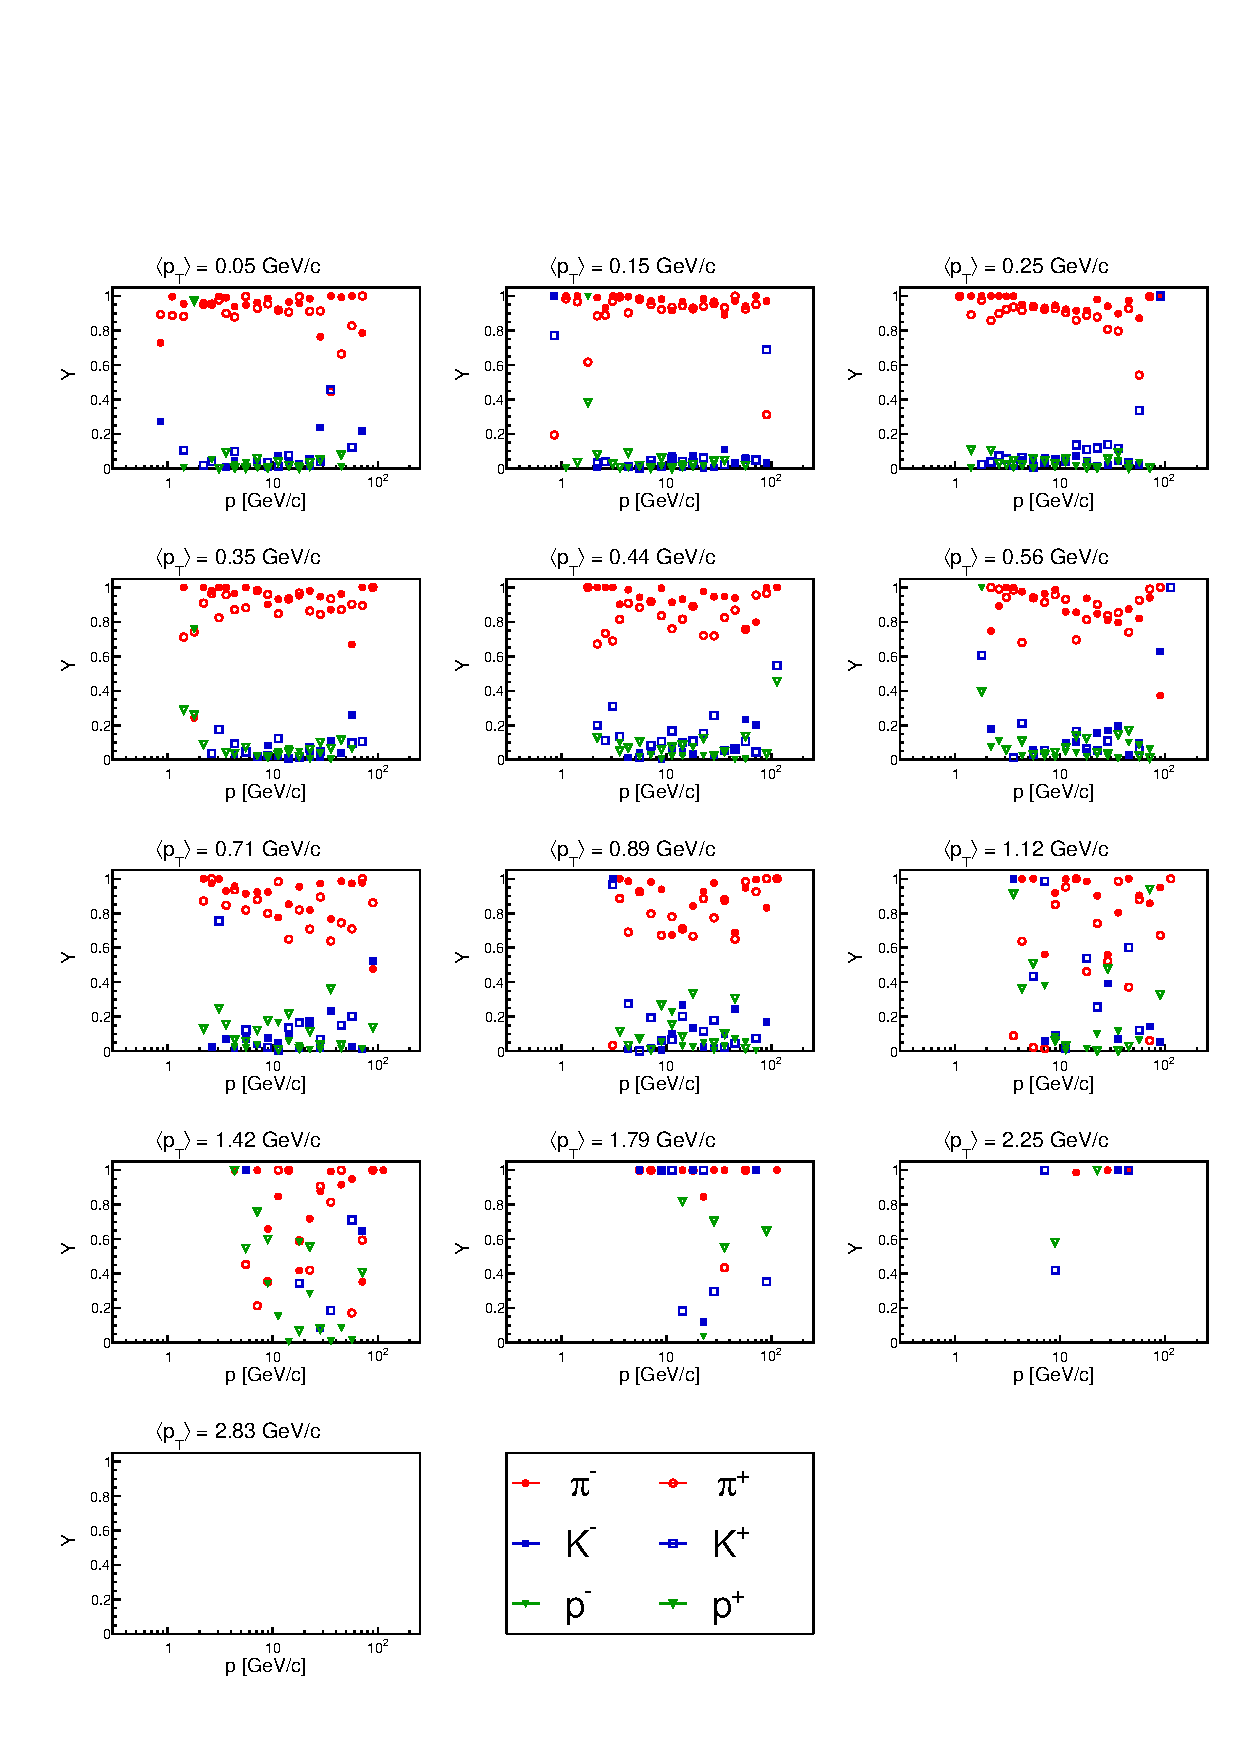
\includegraphics[clip, rviewport=0 0 1 1,width=1.00\textwidth]{dedx/fraction_out_pt_158_v0}
  \caption{Particle fractions obtained from the \dedx fit of the RST and 158 \GeVc dataset, with target removed.}
  \label{fig:hadron:dedx:fit:out158r}
\end{figure}

\begin{figure}
  \centering
  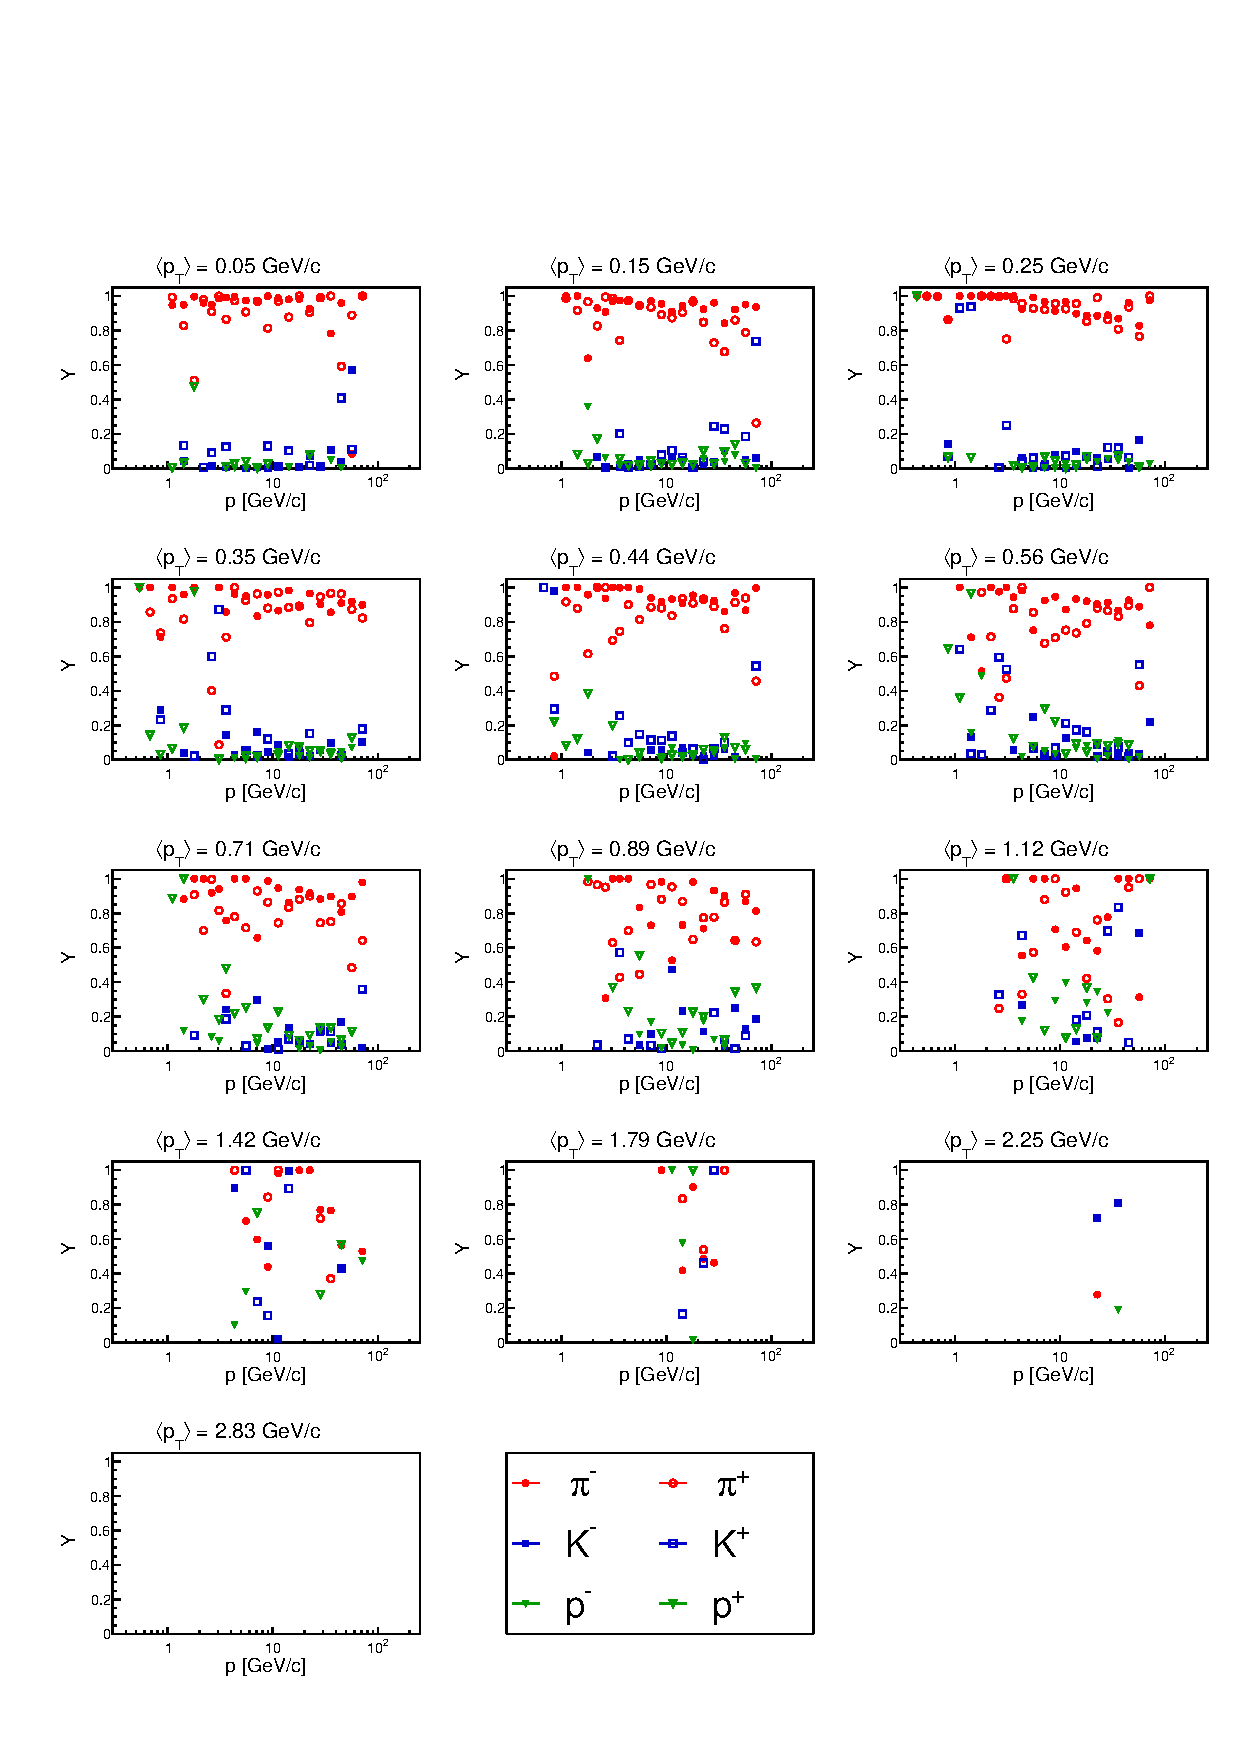
\includegraphics[clip, rviewport=0 0 1 1,width=1.00\textwidth]{dedx/fraction_out_pt_158_v1}
  \caption{Particle fractions obtained from the \dedx fit of the WST and 158 \GeVc dataset, with target inserted.}
  \label{fig:hadron:dedx:fit:out158w}
\end{figure}

\begin{figure}
  \centering
  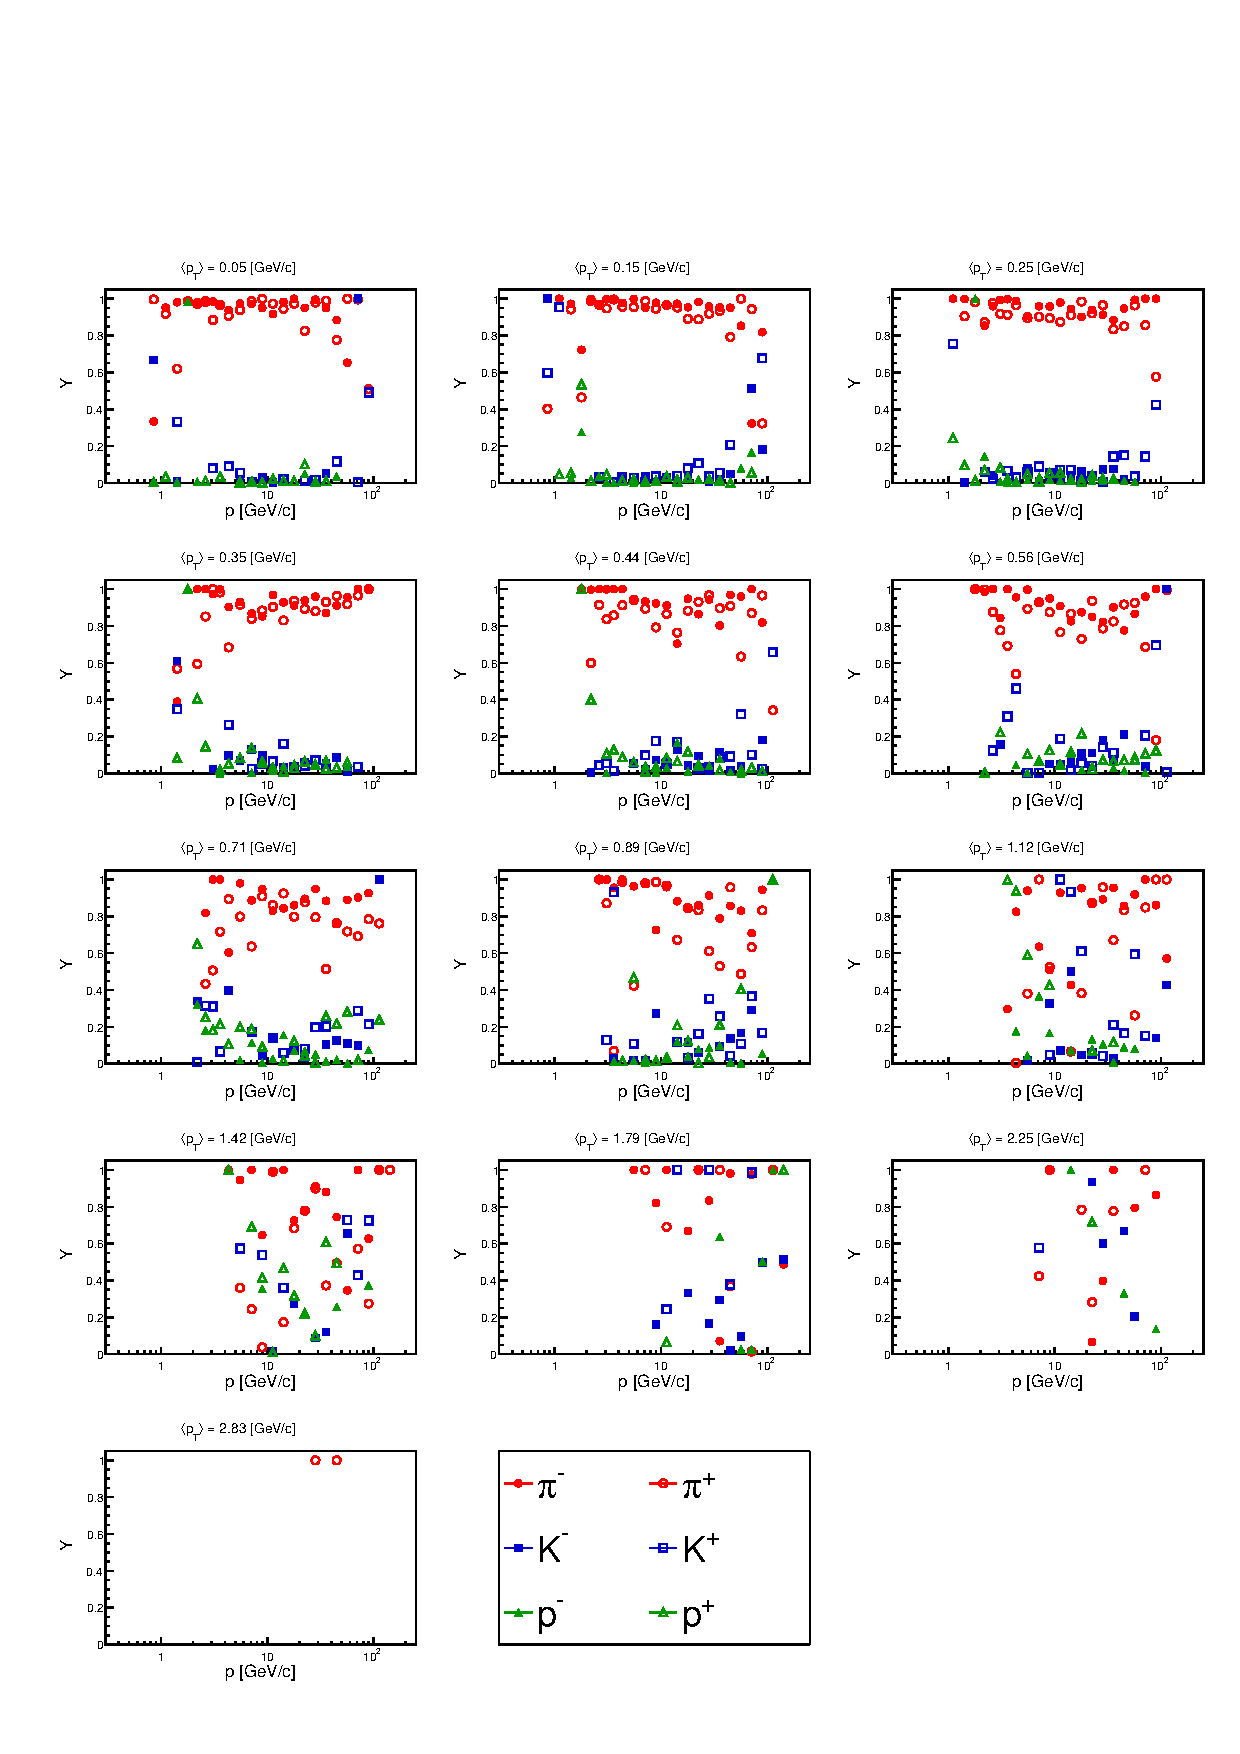
\includegraphics[clip, rviewport=0 0 1 1,width=1.00\textwidth]{dedx/fraction_out_pt_350_v0}
  \caption{Particle fractions obtained from the \dedx fit of the RST and 350 \GeVc dataset, with target inserted.}
  \label{fig:hadron:dedx:fit:out350r}
\end{figure}

\begin{figure}
  \centering
  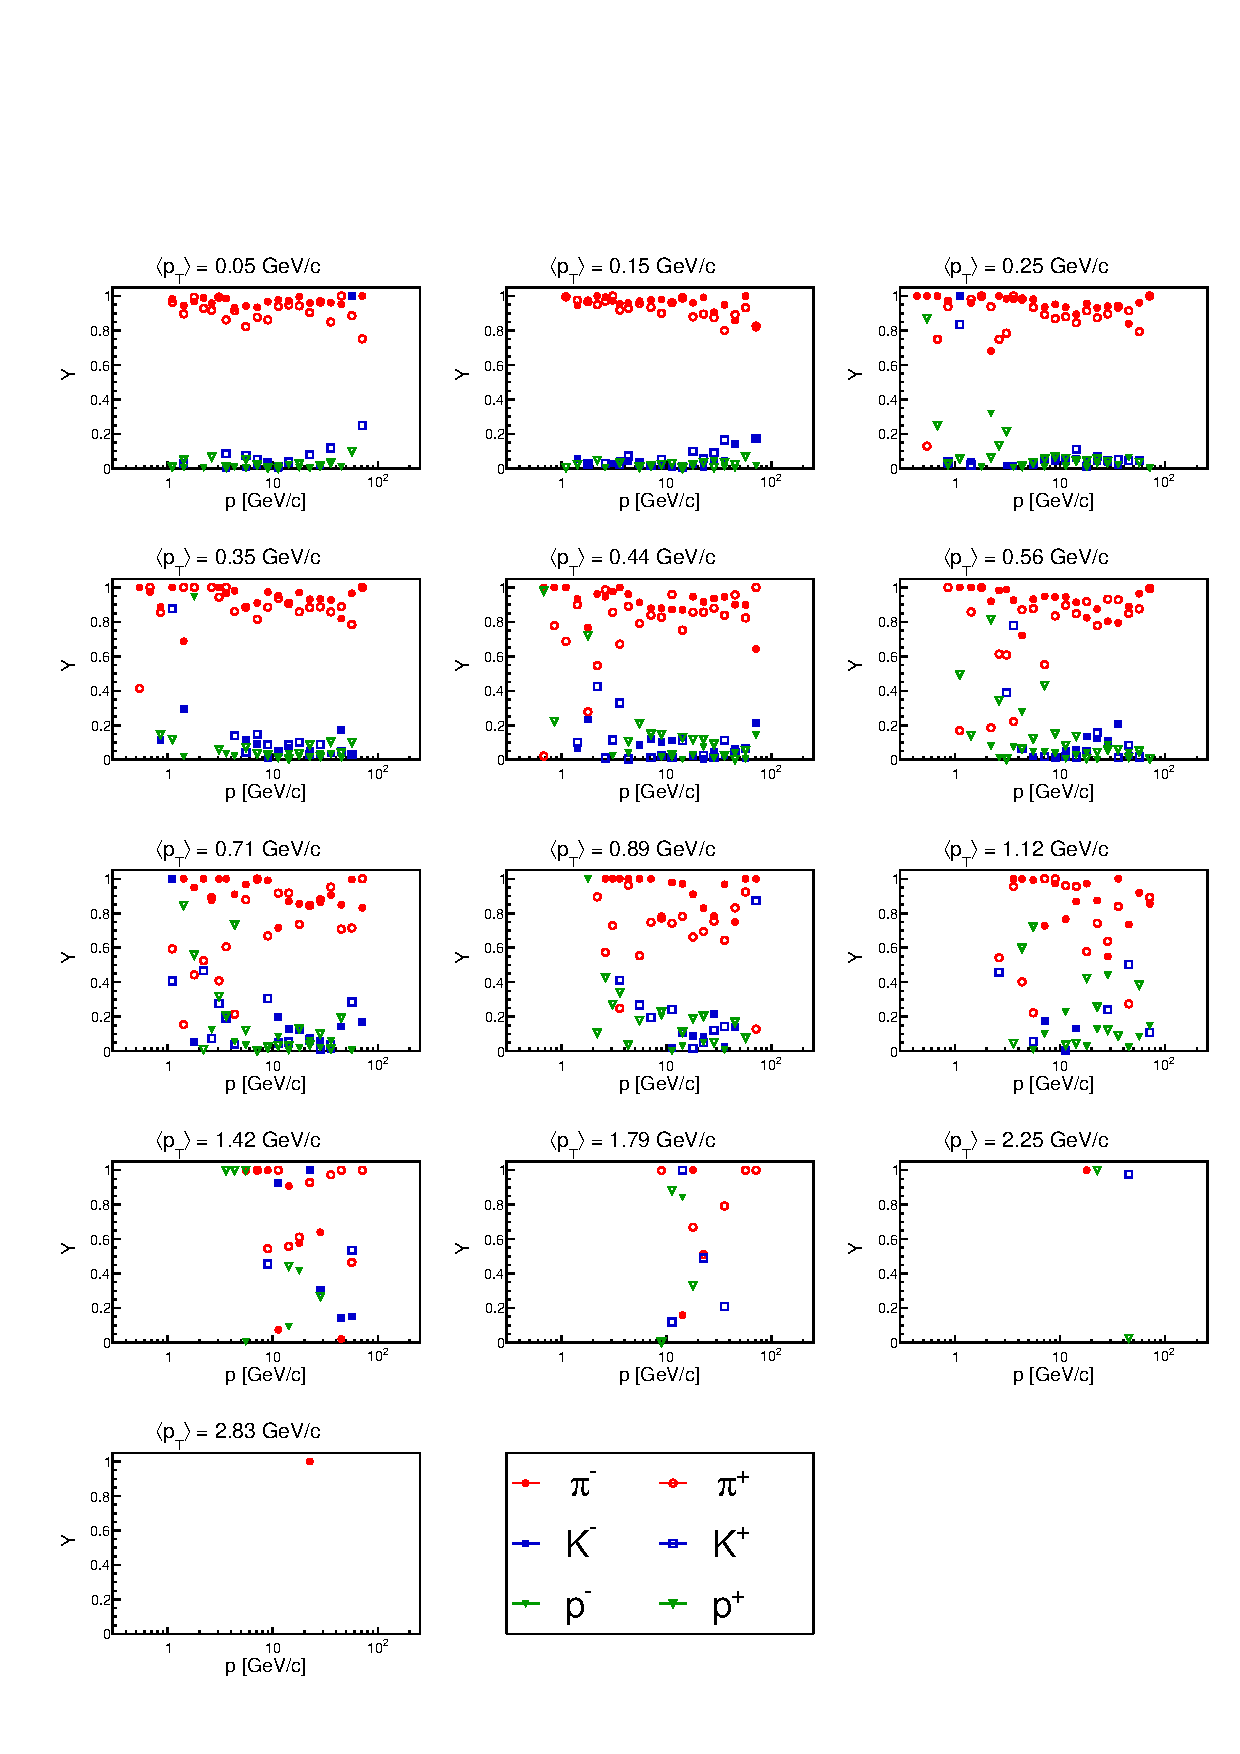
\includegraphics[clip, rviewport=0 0 1 1,width=1.00\textwidth]{dedx/fraction_out_pt_350_v1}
  \caption{Particle fractions obtained from the \dedx fit of the WST and 350 \GeVc dataset, with target inserted.}
  \label{fig:hadron:dedx:fit:out350w}
\end{figure}



%%%%%%%%%%% DECAY DIST CUT %%%%%%%%%%%%%%%%%%
\begin{figure}
  \centering
  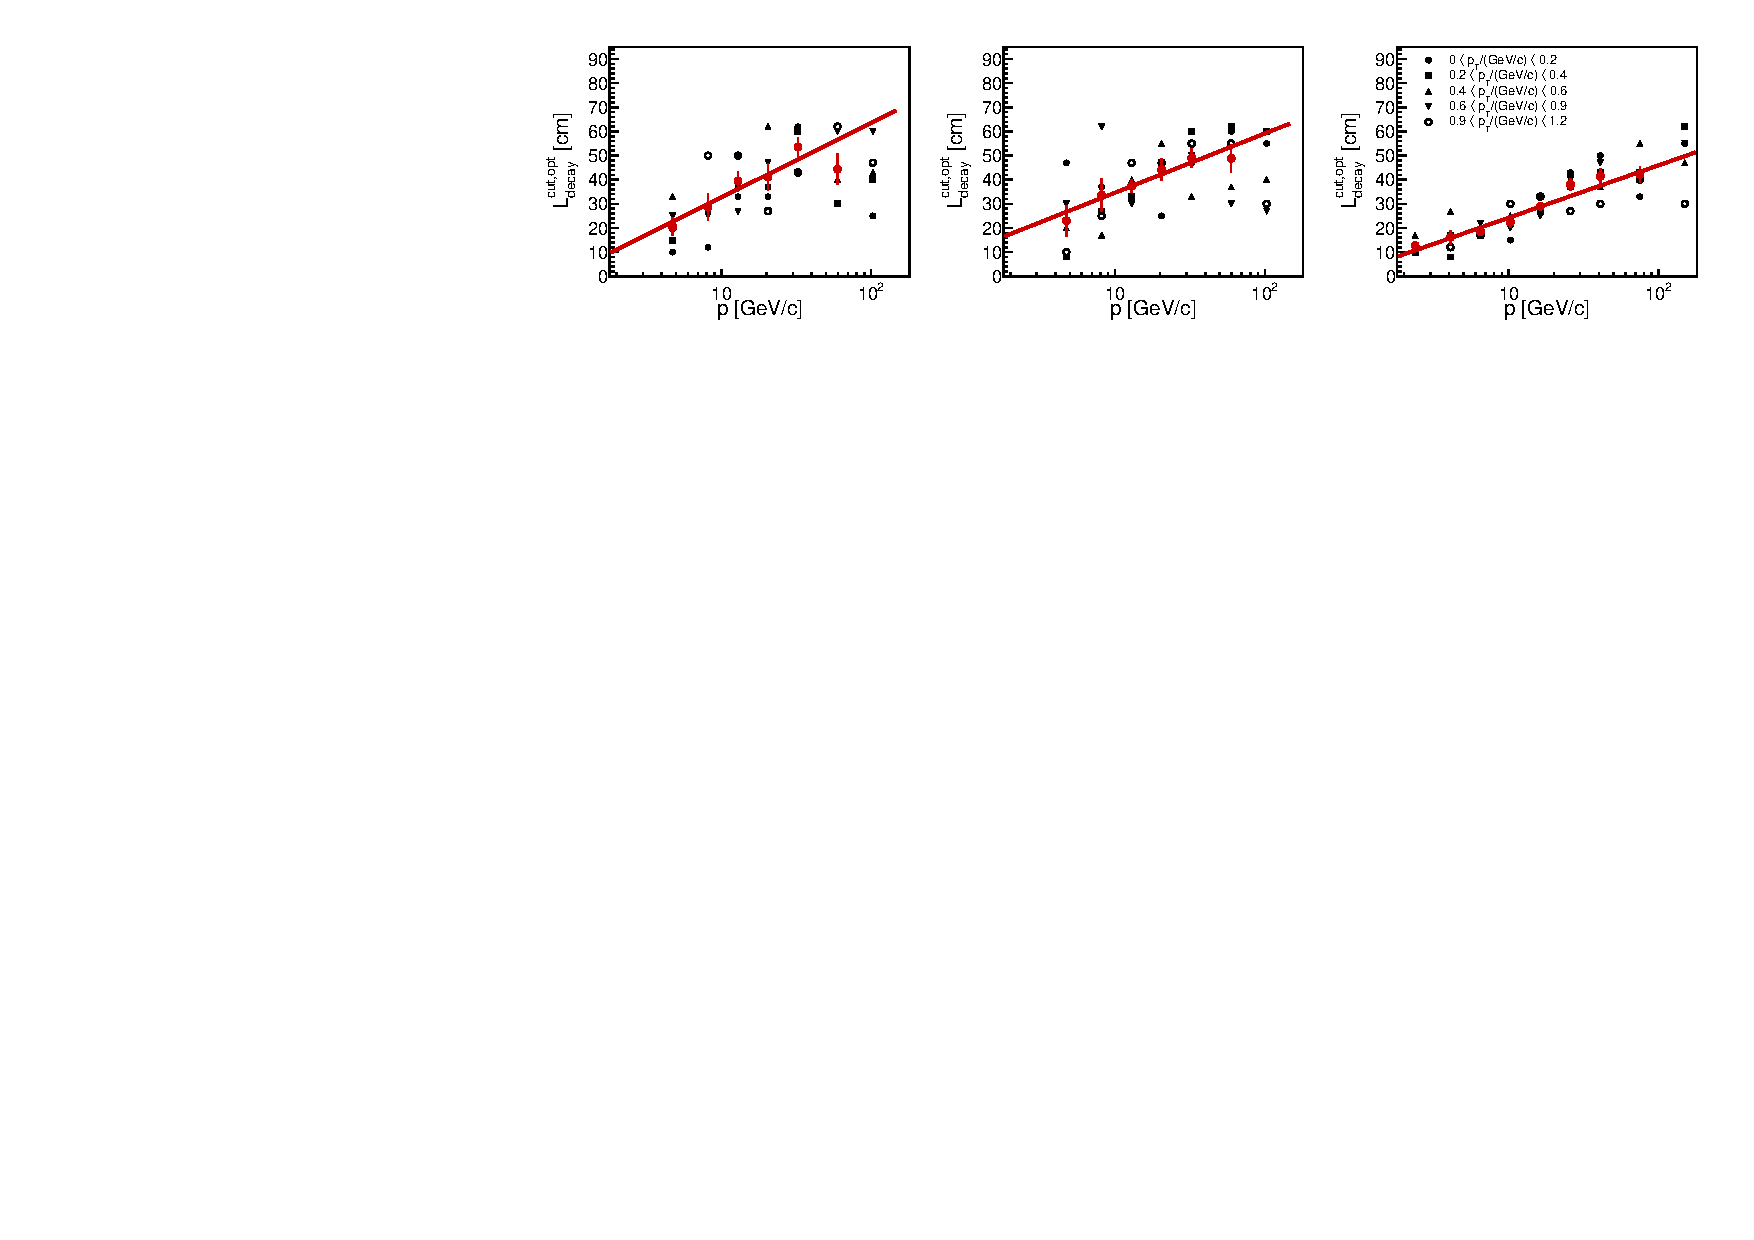
\includegraphics[clip, rviewport=0 0 1 1,width=0.99\textwidth]{vzero/cut_dist_Data350}
  
  \caption{Optimization of the \decaydistmin for the 350 \GeVc dataset. The plot on left, middle and right shows \lamb, \antilamb and \kzeros, respectively.}
  \label{fig:hadron:vzero:cuts:decaydist:350}
\end{figure}

\clearpage

%%%%%%%%%%% CHI SQ %%%%%%%%%%%%%%%%%%
\begin{figure}
  \centering
  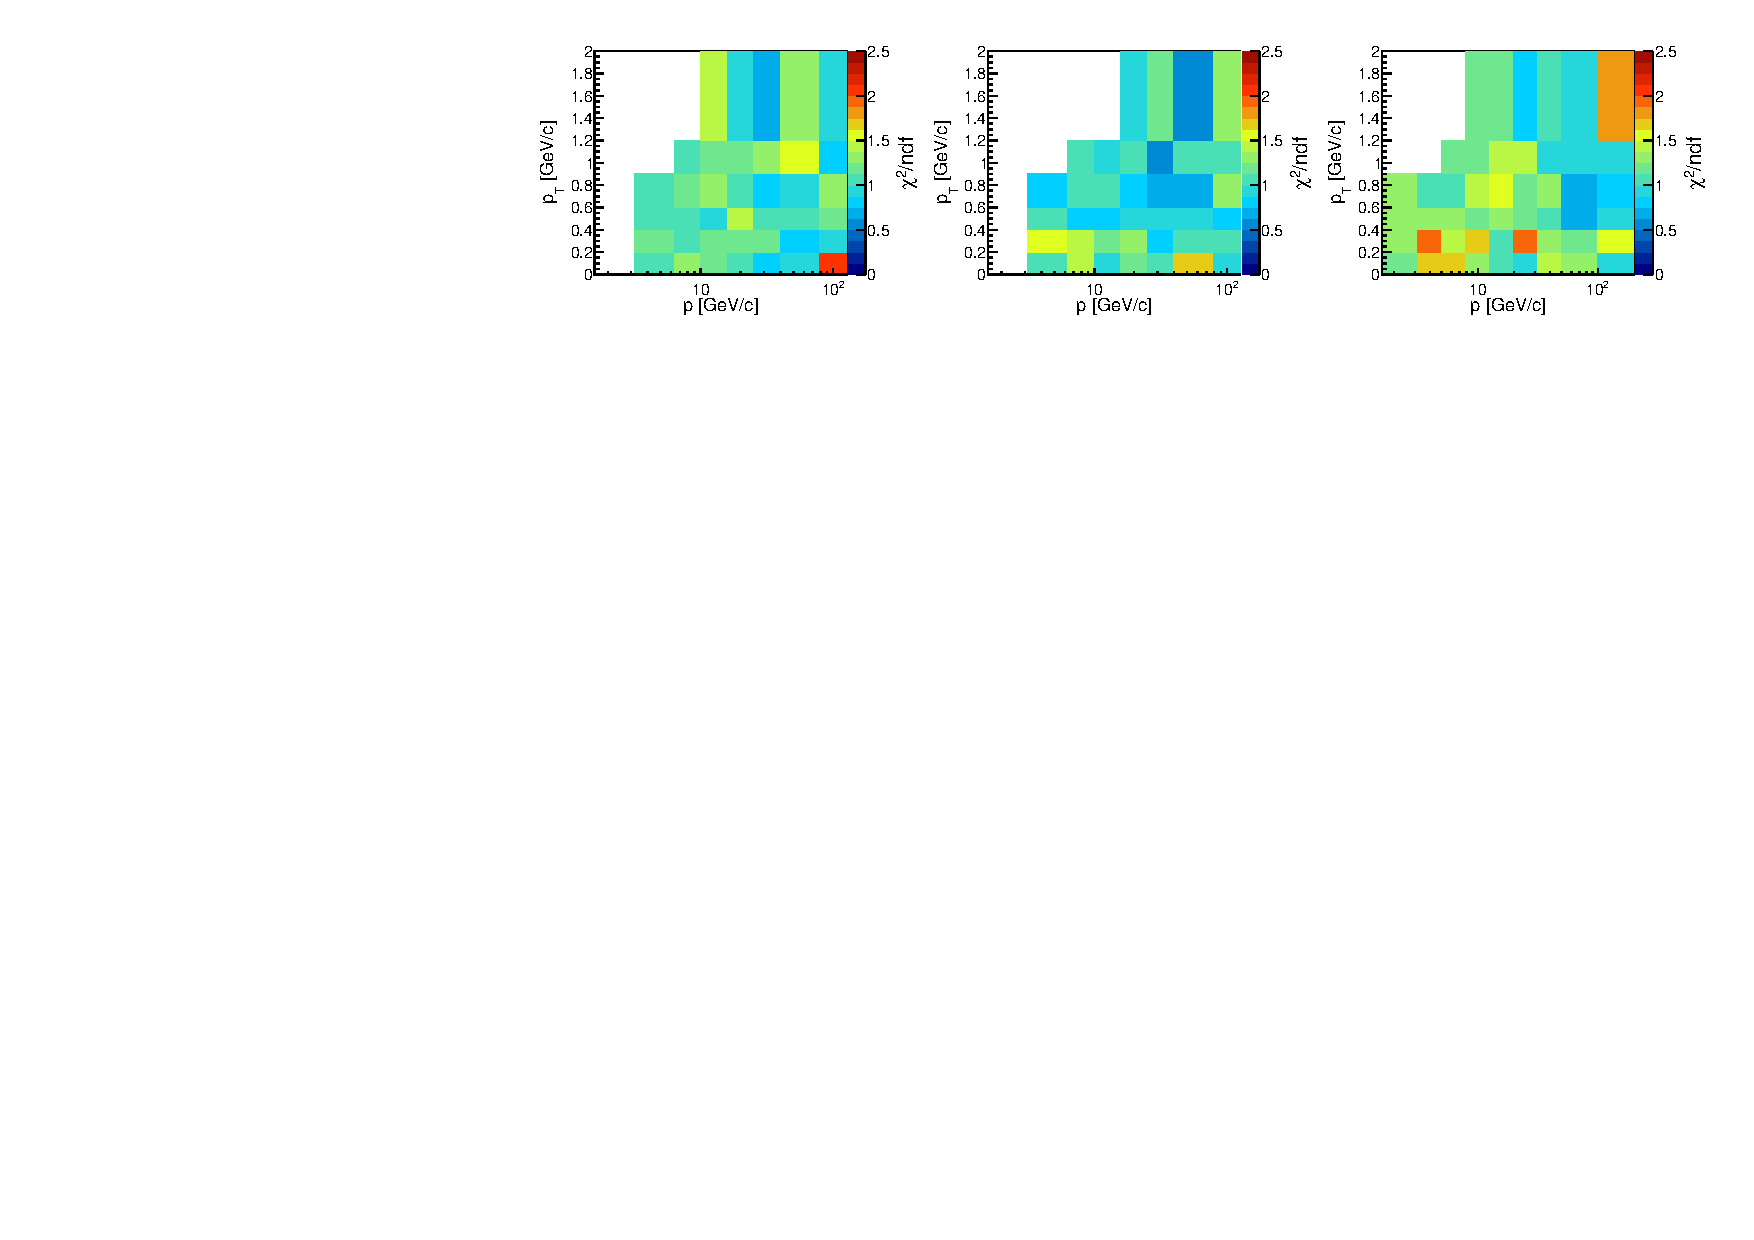
\includegraphics[clip, rviewport=0 0 1 1,width=0.99\textwidth]{vzero/chisq_Data350_t0_ph1}
  
  \caption{}
  \label{fig:hadron:vzero:signal:chi:350}
\end{figure}


%%%%%%%%%%% EXTRACTED SIGNAL %%%%%%%%%%%%%%%%%%
\begin{figure}
  \centering
  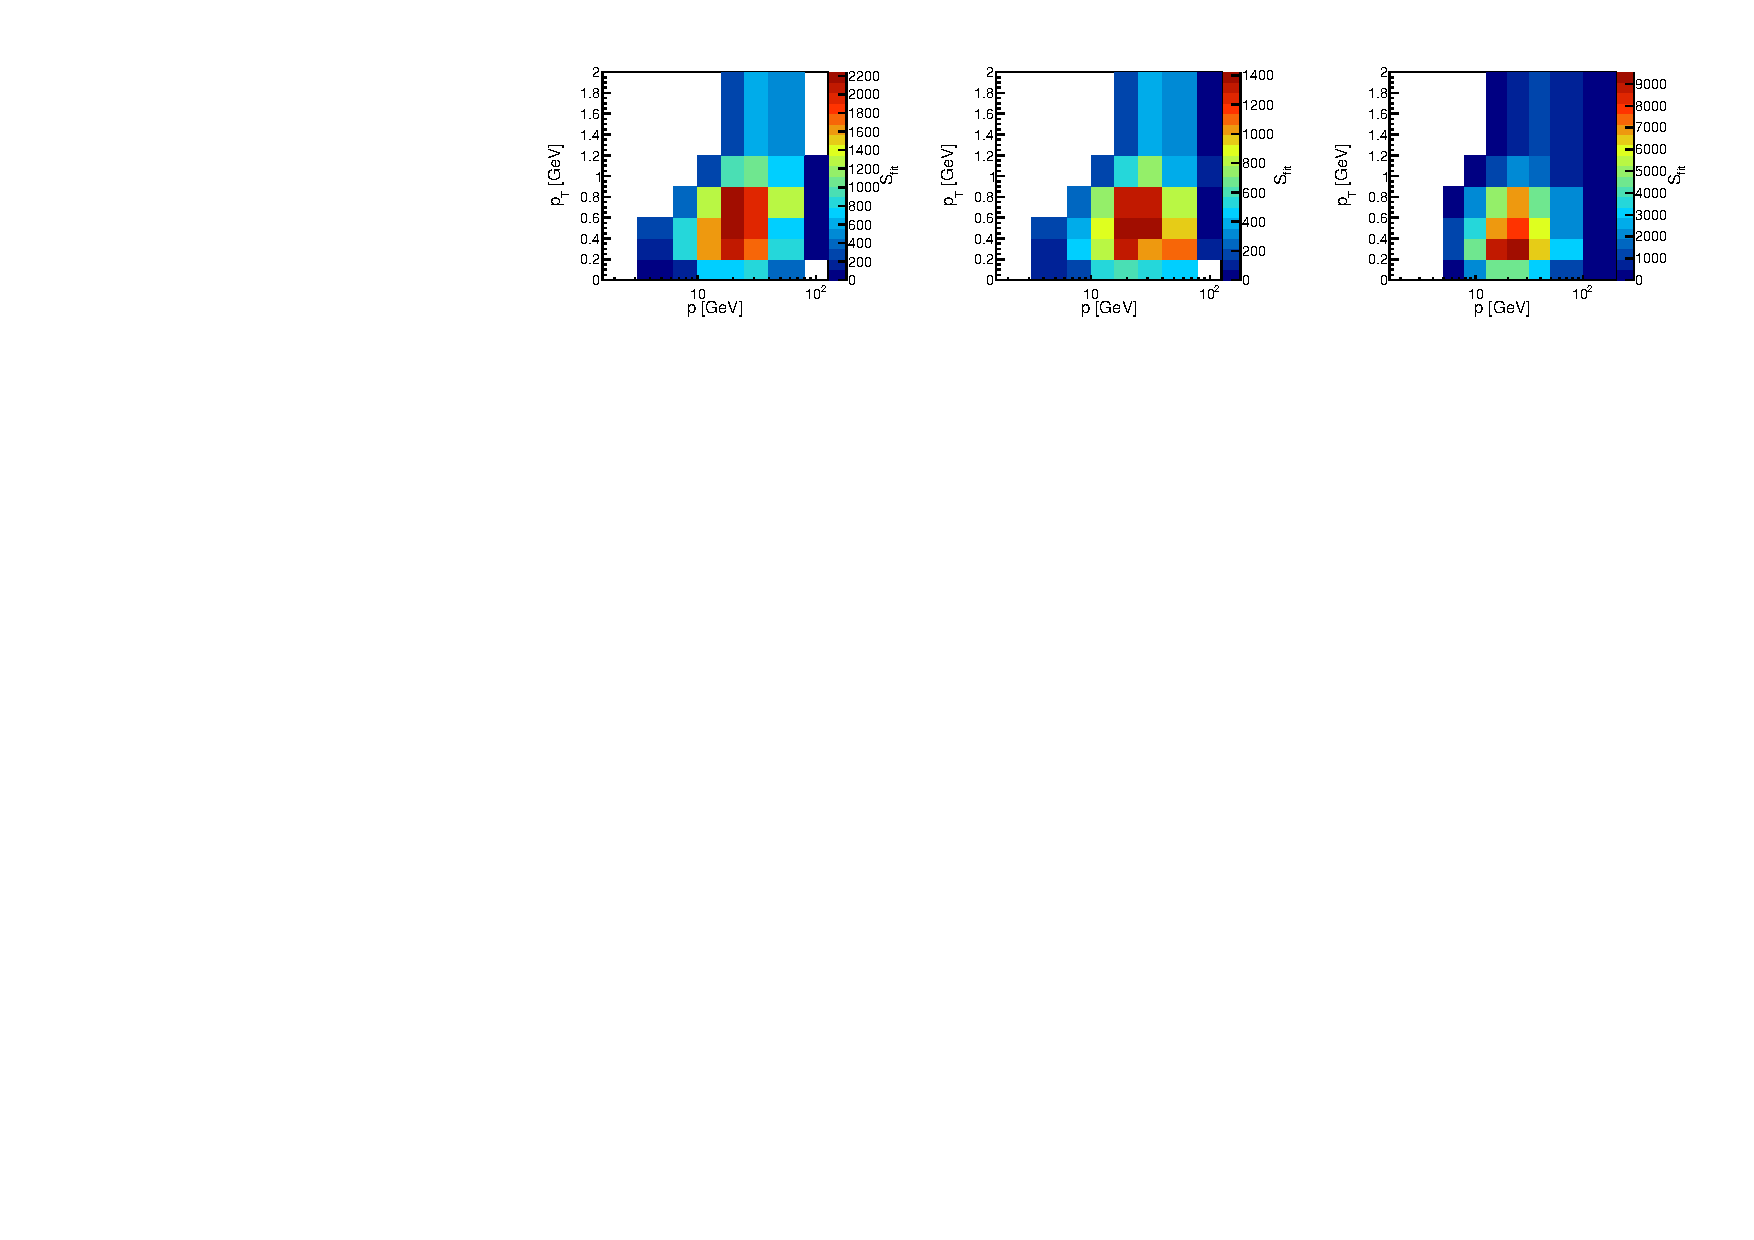
\includegraphics[clip, rviewport=0 0 1 1,width=0.99\textwidth]{vzero/signal_Data350_t0}
  
  \caption{}
  \label{fig:hadron:vzero:signal:extracted:350in}
\end{figure}

%%%%%%%%%%% EXTRACTED SIGNAL %%%%%%%%%%%%%%%%%%
\begin{figure}
  \centering
  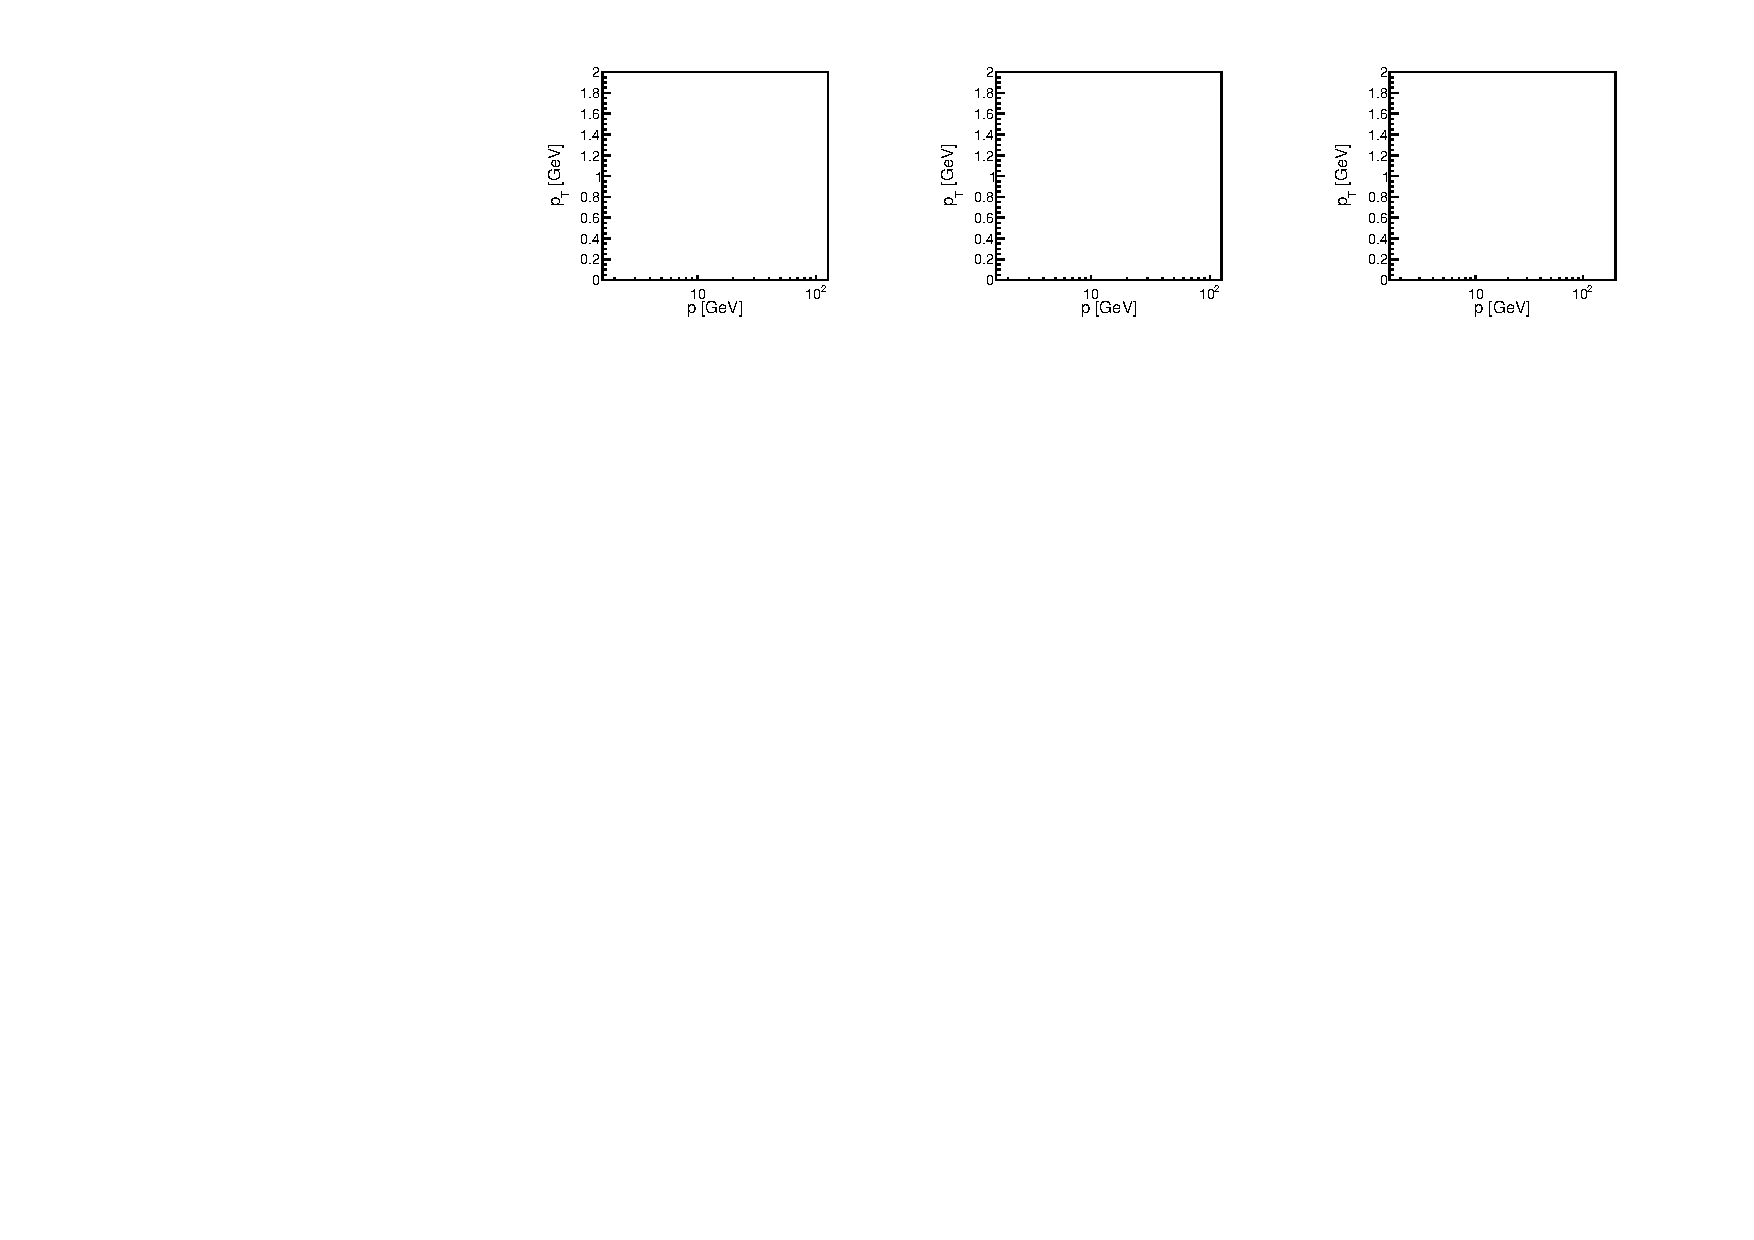
\includegraphics[clip, rviewport=0 0 1 1,width=0.99\textwidth]{vzero/signal_Data350_t1}
  
  \caption{}
  \label{fig:hadron:vzero:signal:extracted:350out}
\end{figure}


%%%%%%%%%%% DIST %%%%%%%%%%%%%%%%%%
\begin{figure}[!ht]
  \centering
  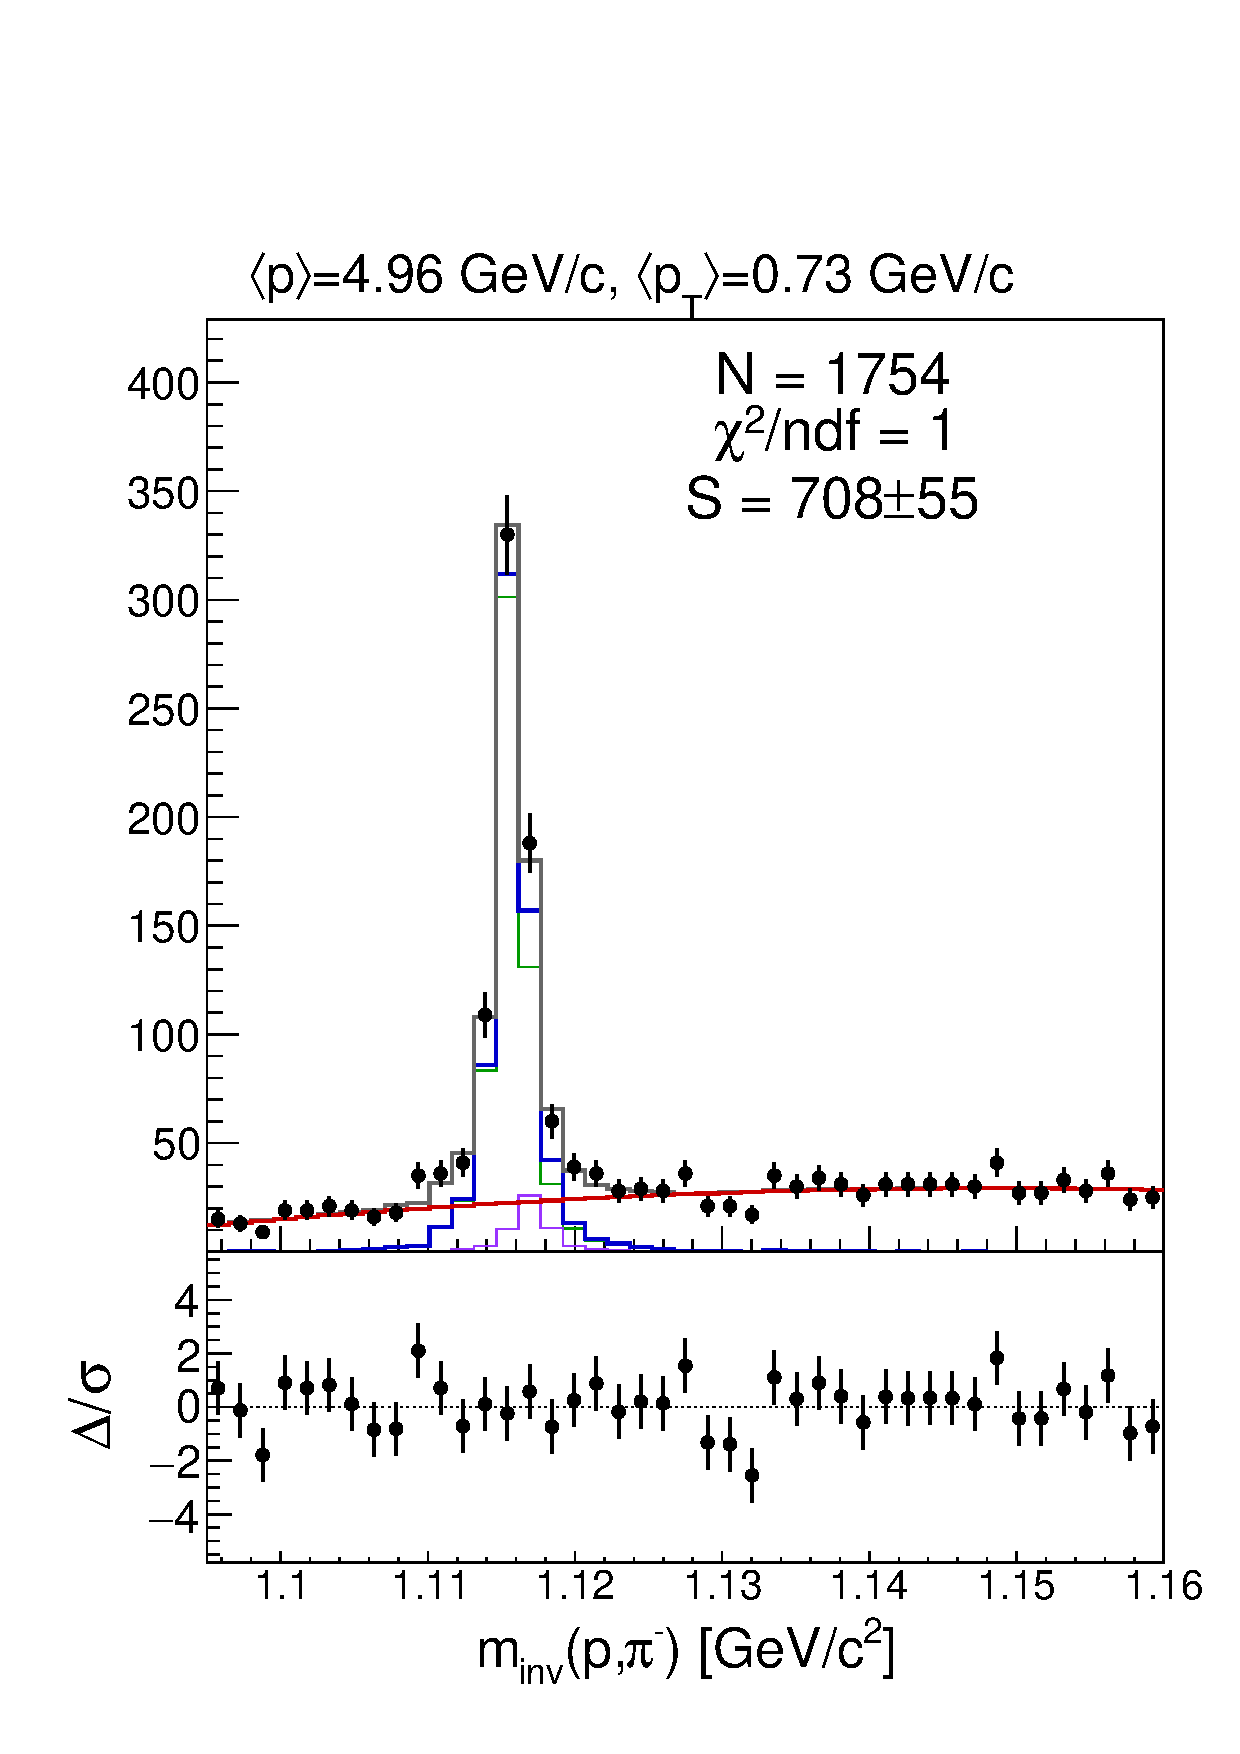
\includegraphics[clip, rviewport=0 0 1 1,width=0.32\textwidth]{vzero/mass_Data350_t0_ph1_h0_x1_y3}
  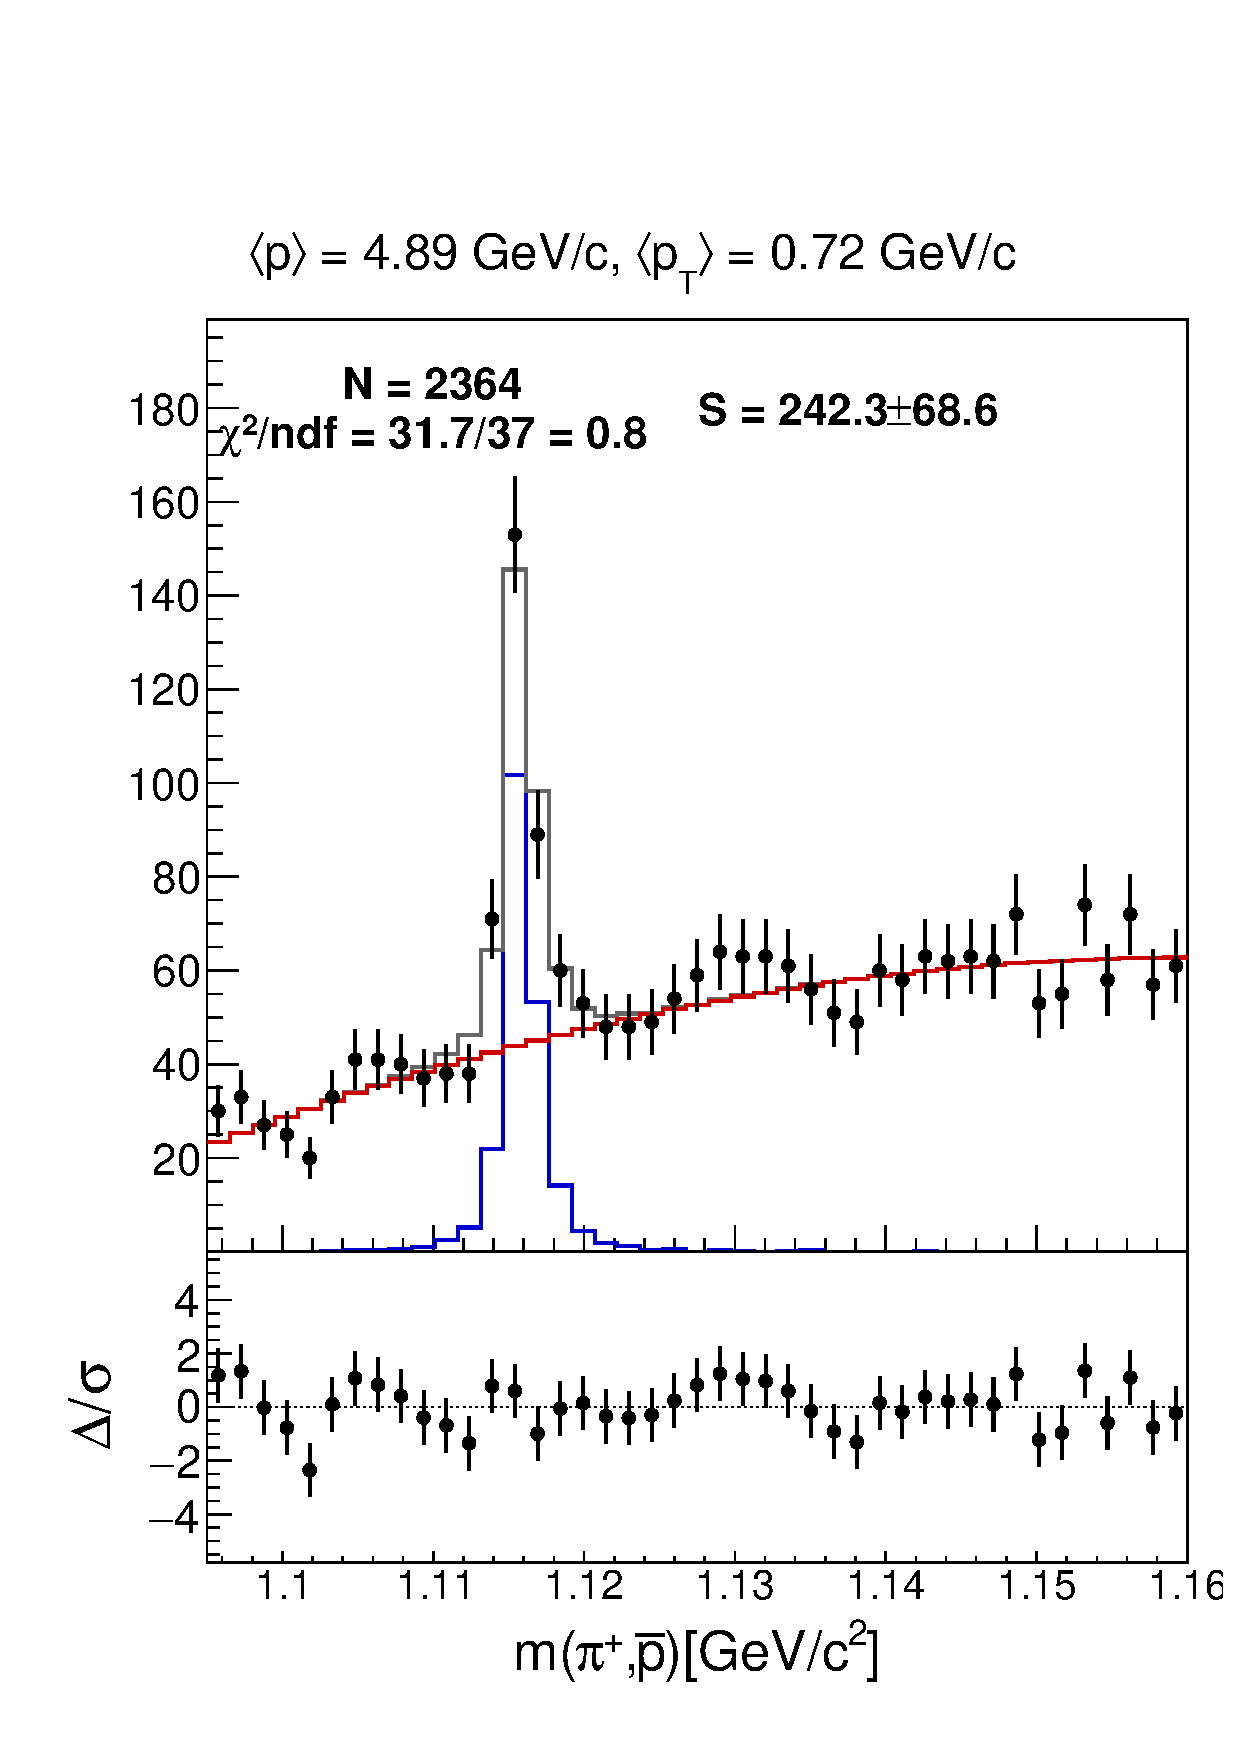
\includegraphics[clip, rviewport=0 0 1 1,width=0.32\textwidth]{vzero/mass_Data350_t0_ph1_h1_x1_y3}
  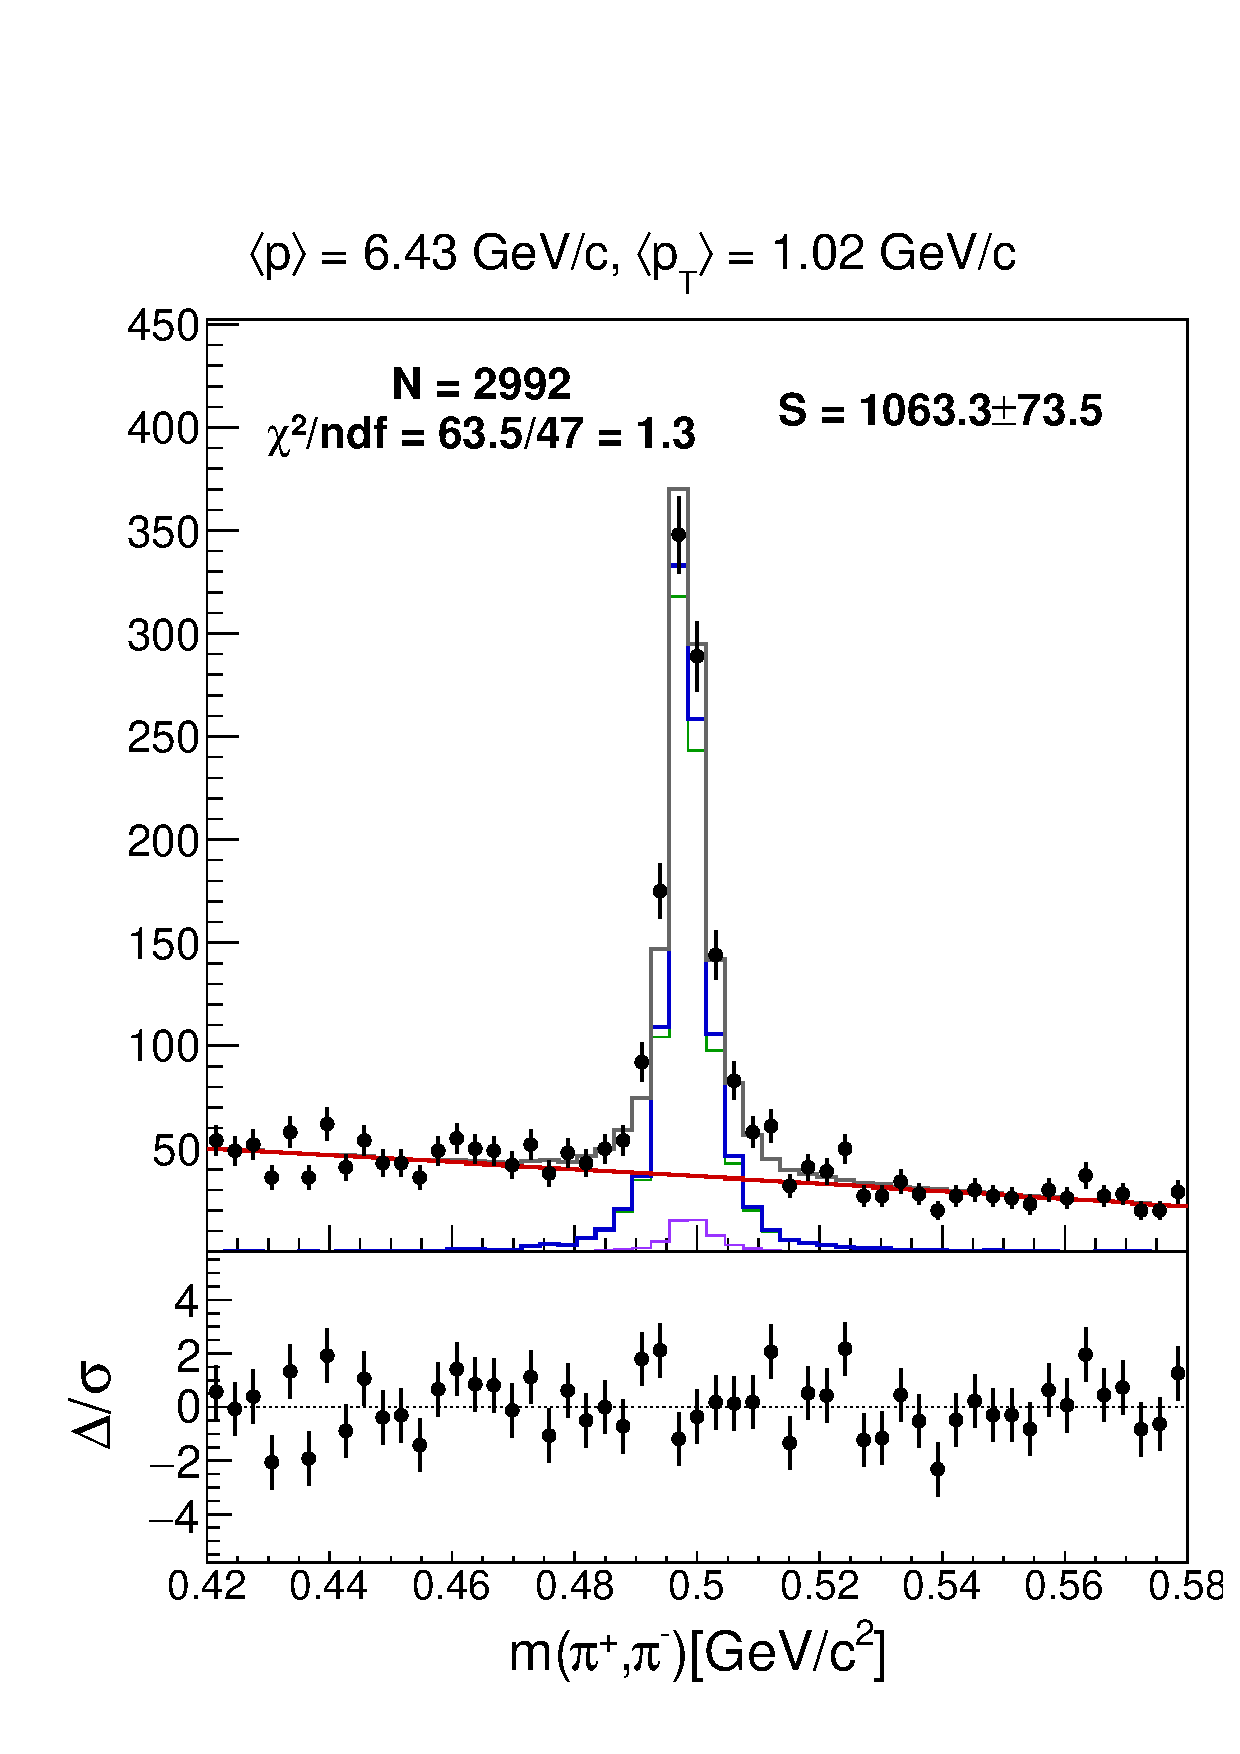
\includegraphics[clip, rviewport=0 0 1 1,width=0.32\textwidth]{vzero/mass_Data350_t0_ph1_h2_x2_y4}

  \vspace{0.5cm}
    
  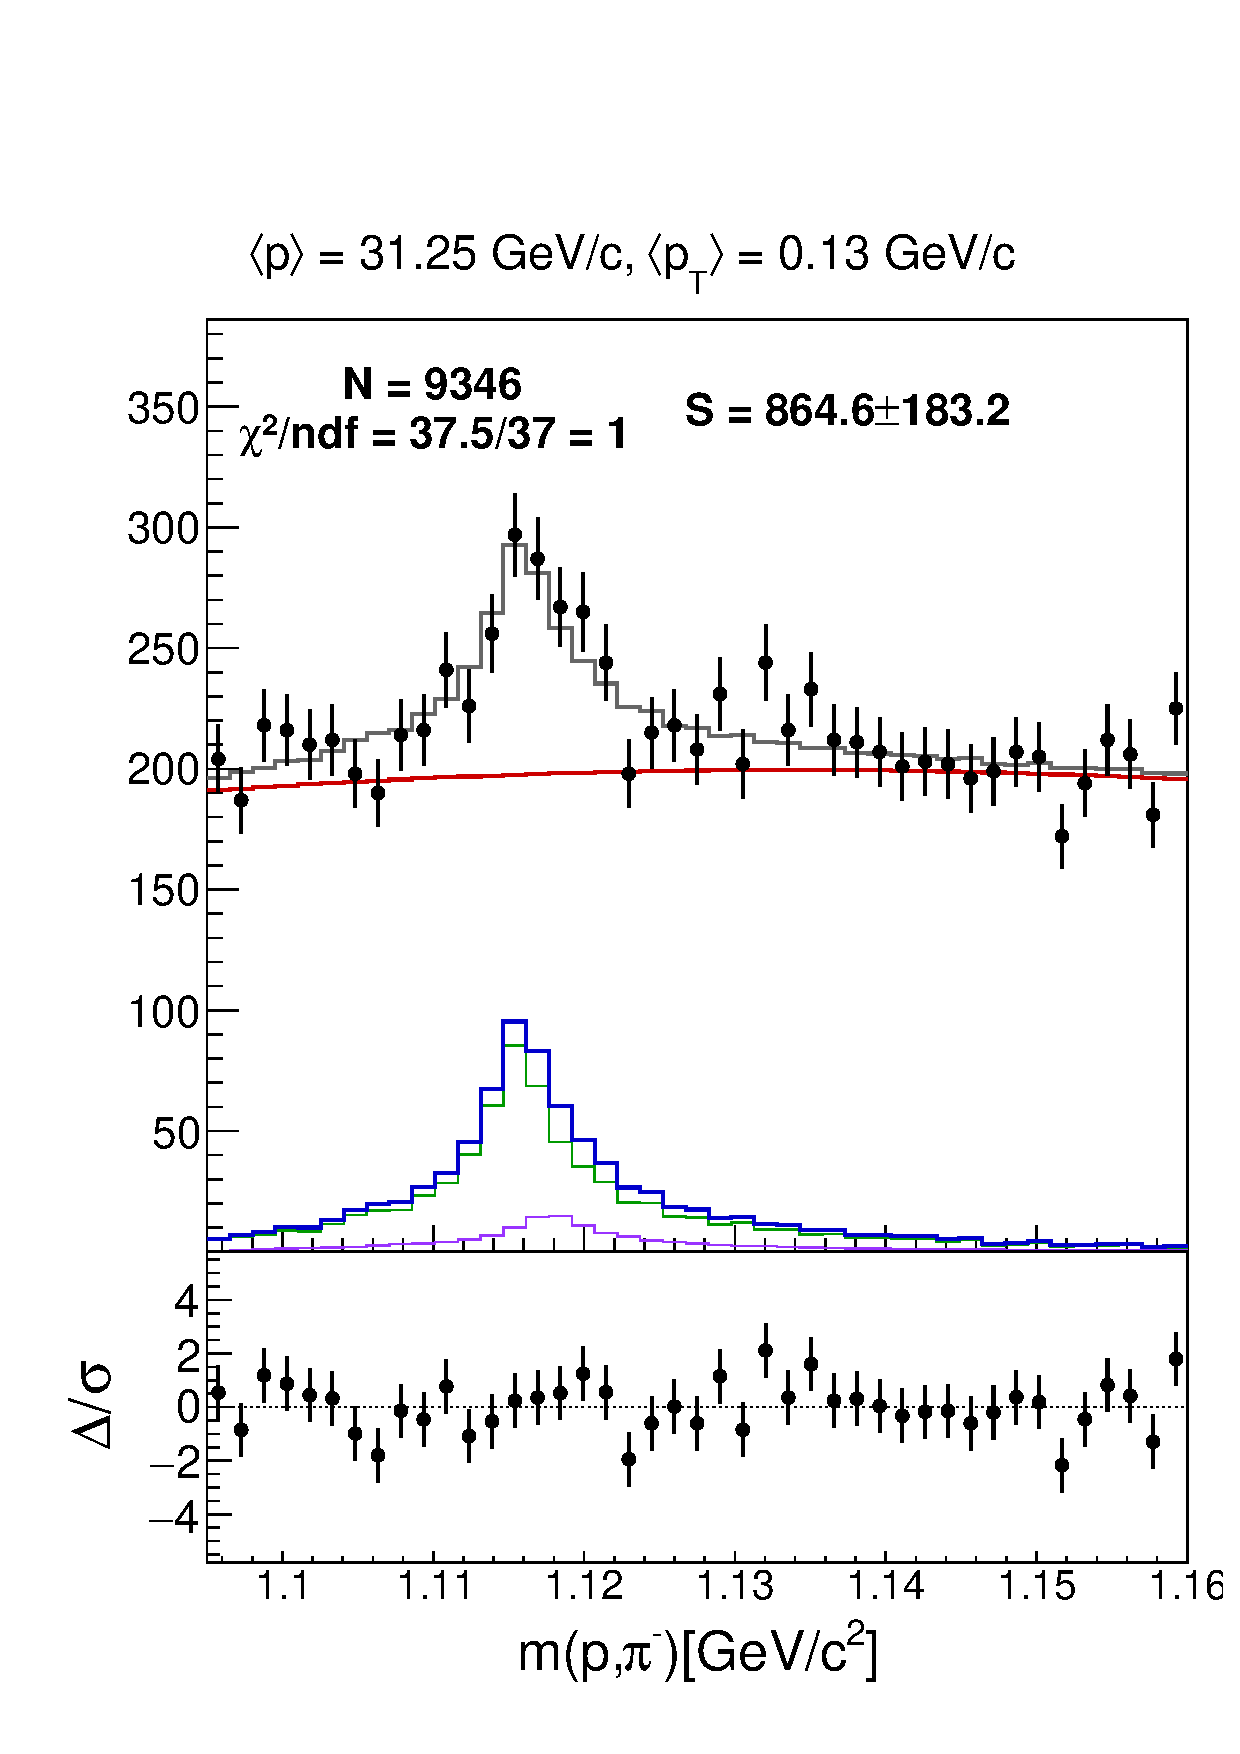
\includegraphics[clip, rviewport=0 0 1 1,width=0.32\textwidth]{vzero/mass_Data350_t0_ph1_h0_x5_y0}
  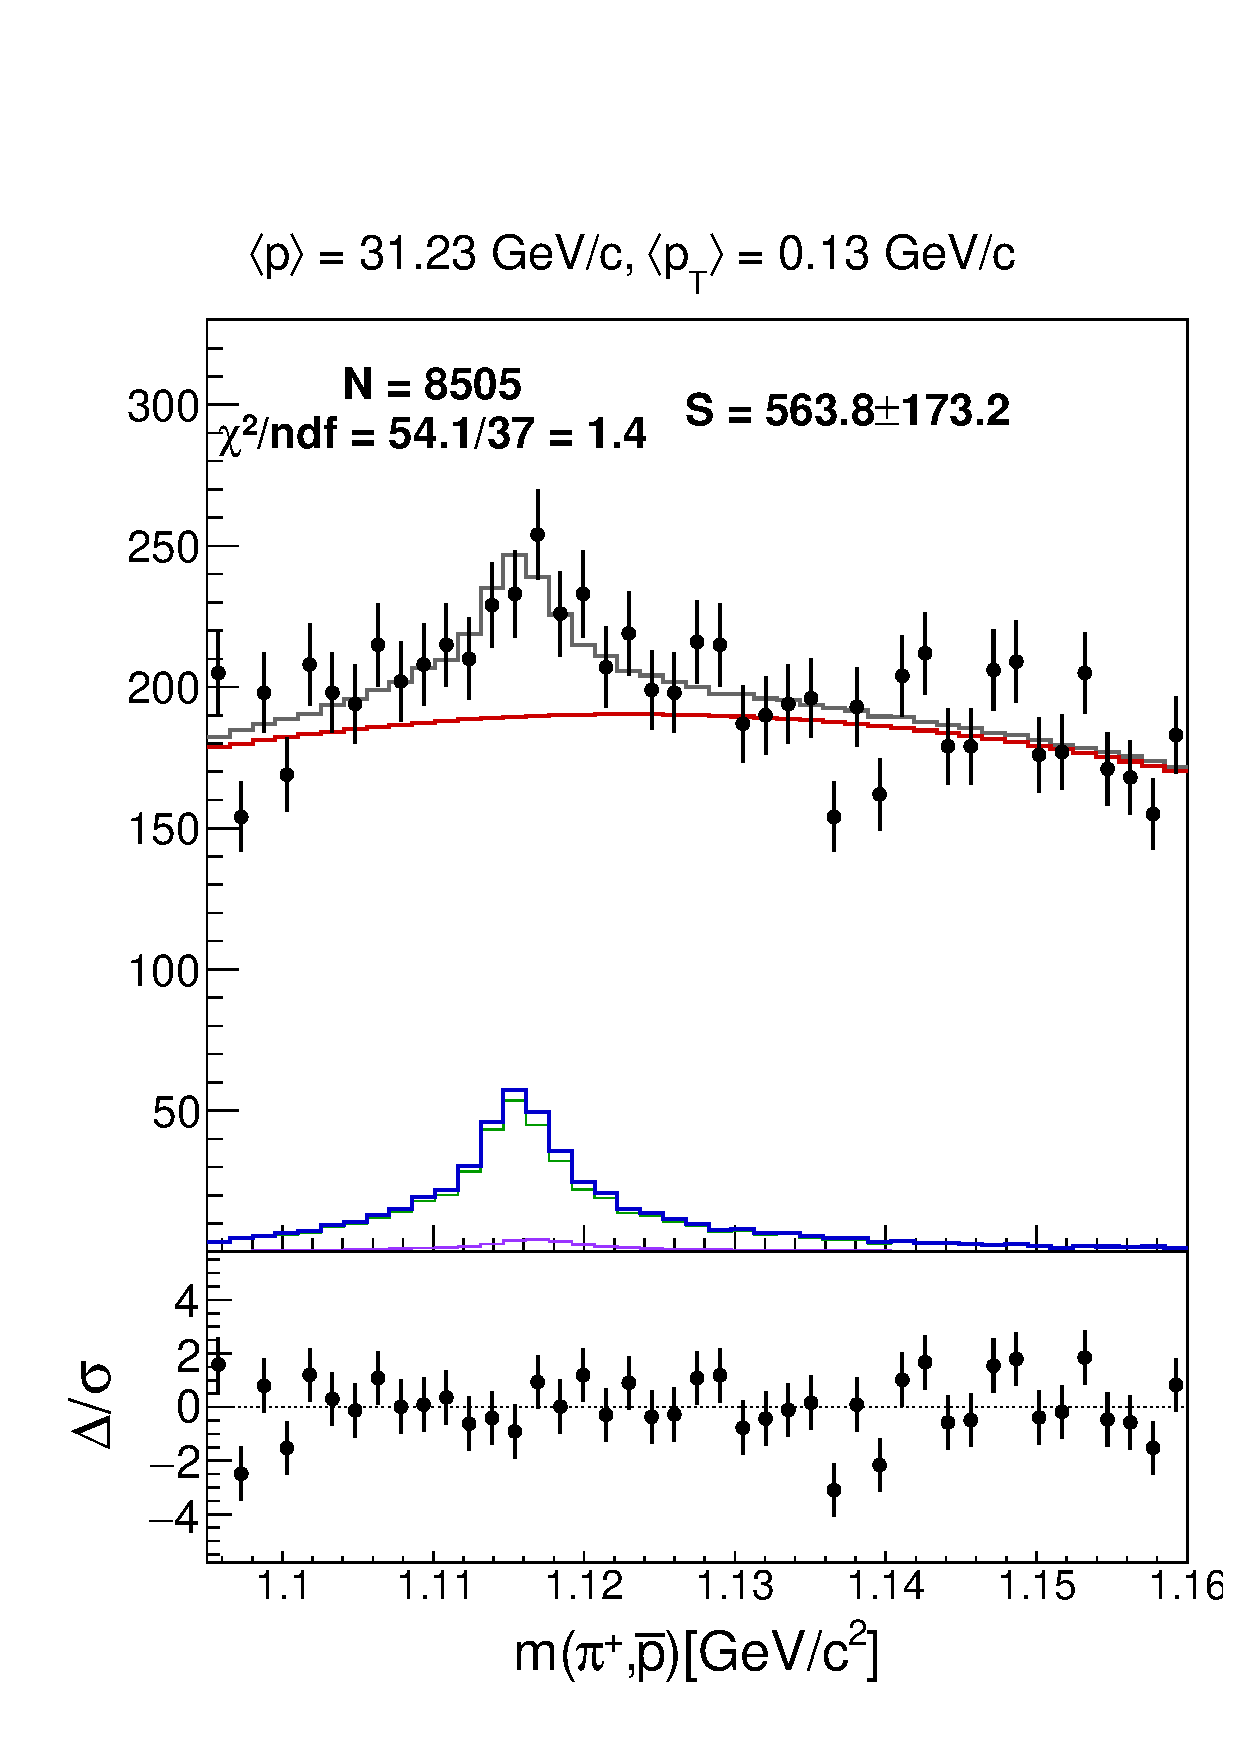
\includegraphics[clip, rviewport=0 0 1 1,width=0.32\textwidth]{vzero/mass_Data350_t0_ph1_h1_x5_y0}
  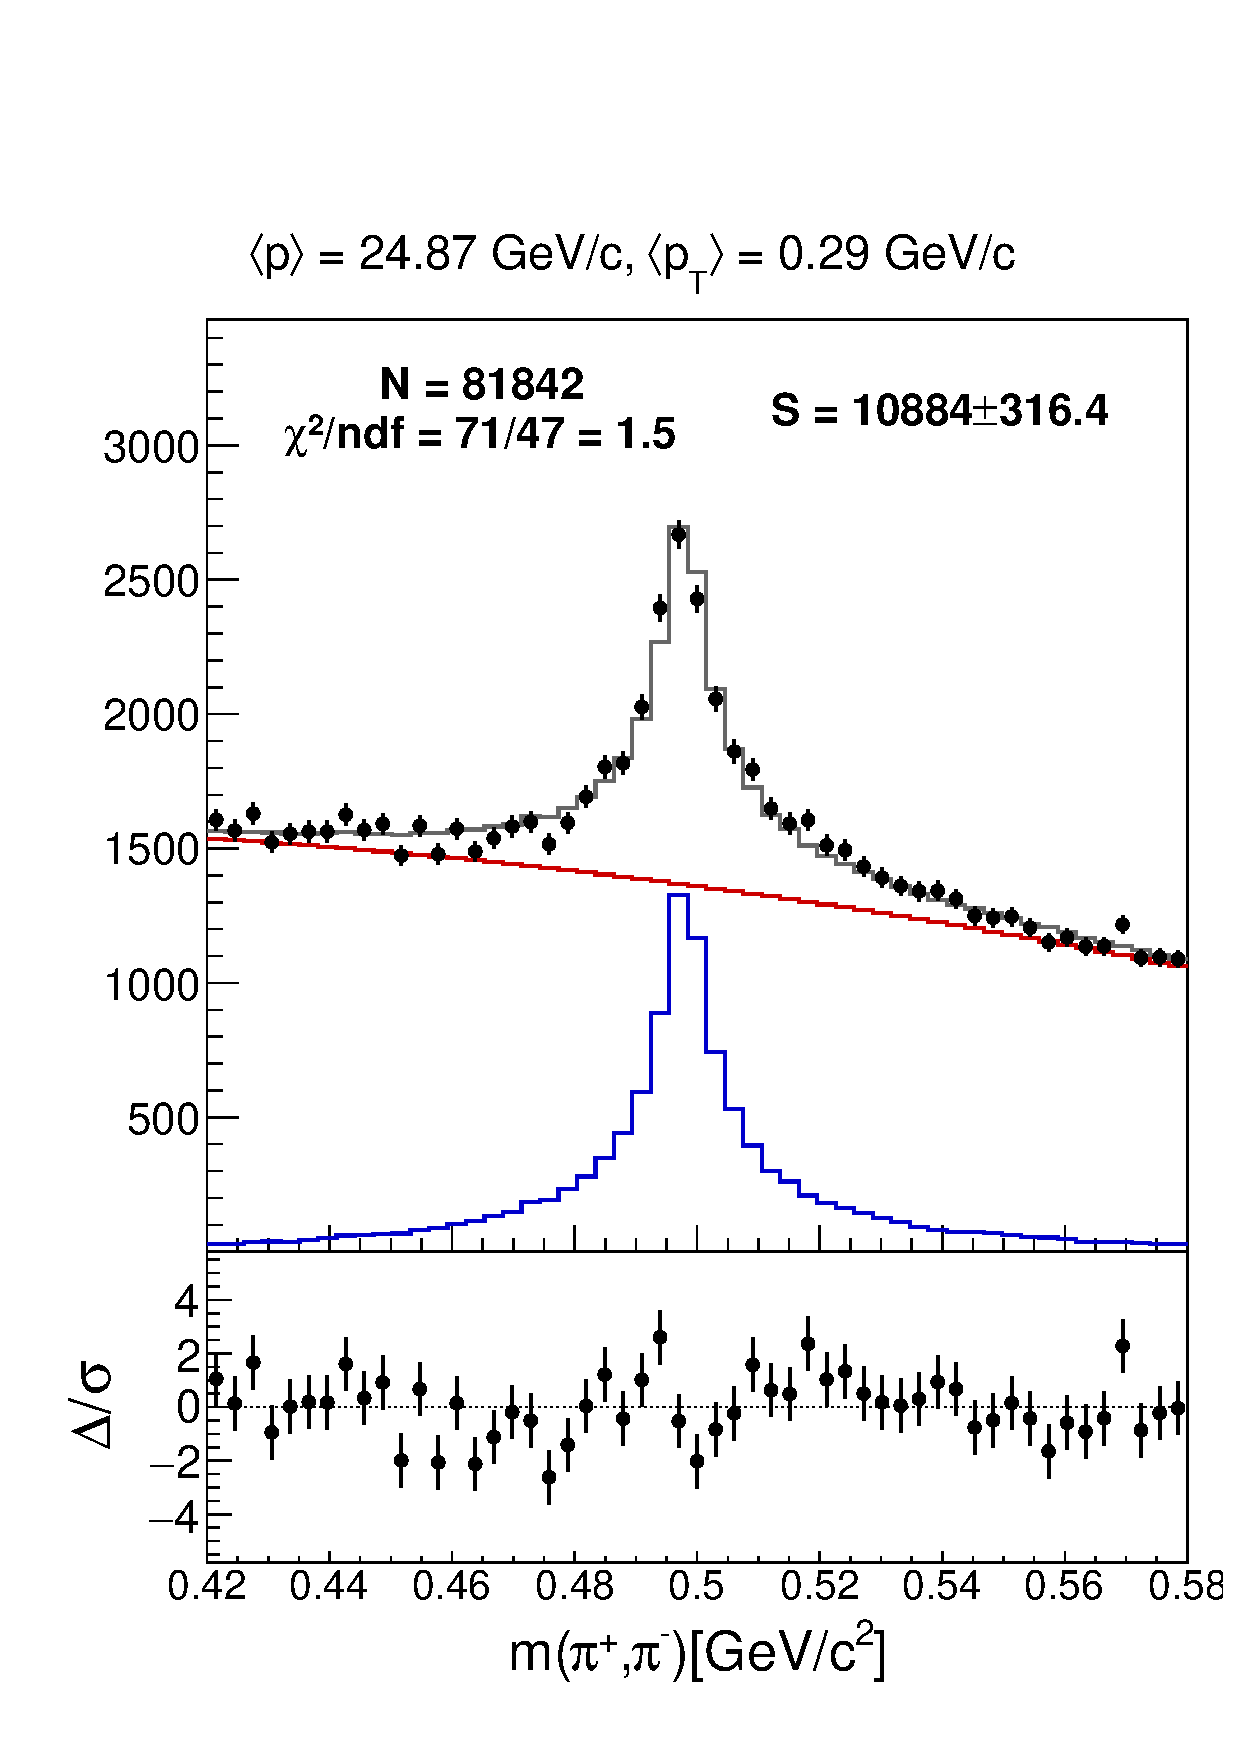
\includegraphics[clip, rviewport=0 0 1 1,width=0.32\textwidth]{vzero/mass_Data350_t0_ph1_h2_x5_y1}

  
  \caption{Examples of the fitted \minv distributions for the 350 \GeVc dataset. The plot on left, middle and right shows \lamb, \antilamb and \kzeros, respectively.}
  \label{fig:hadron:vzero:signal:dist:350:in}
\end{figure}



%%%%%%%%%%% DIST %%%%%%%%%%%%%%%%%%
\begin{figure}[!ht]
  \centering
  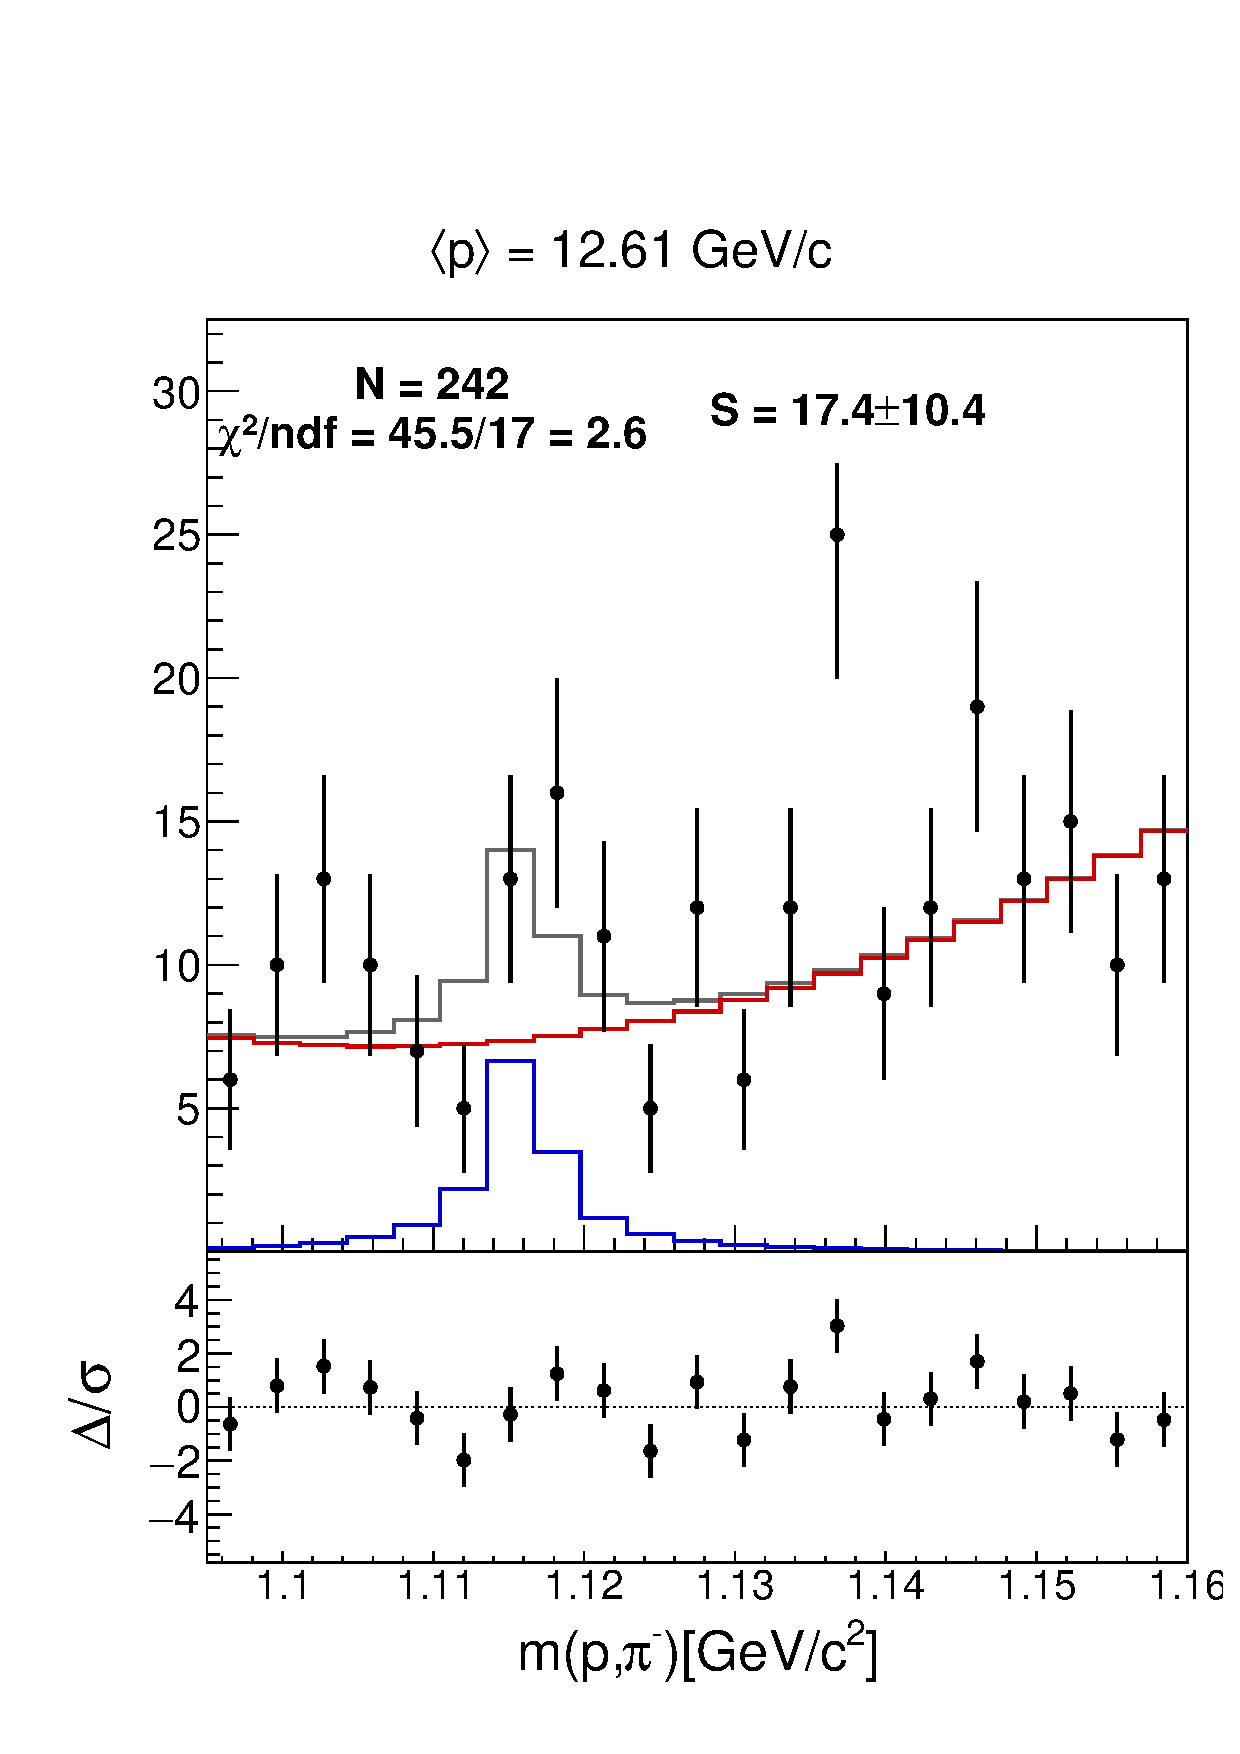
\includegraphics[clip, rviewport=0 0 1 1,width=0.32\textwidth]{vzero/mass_Data350_t1_ph0_h0_x3_y0}
  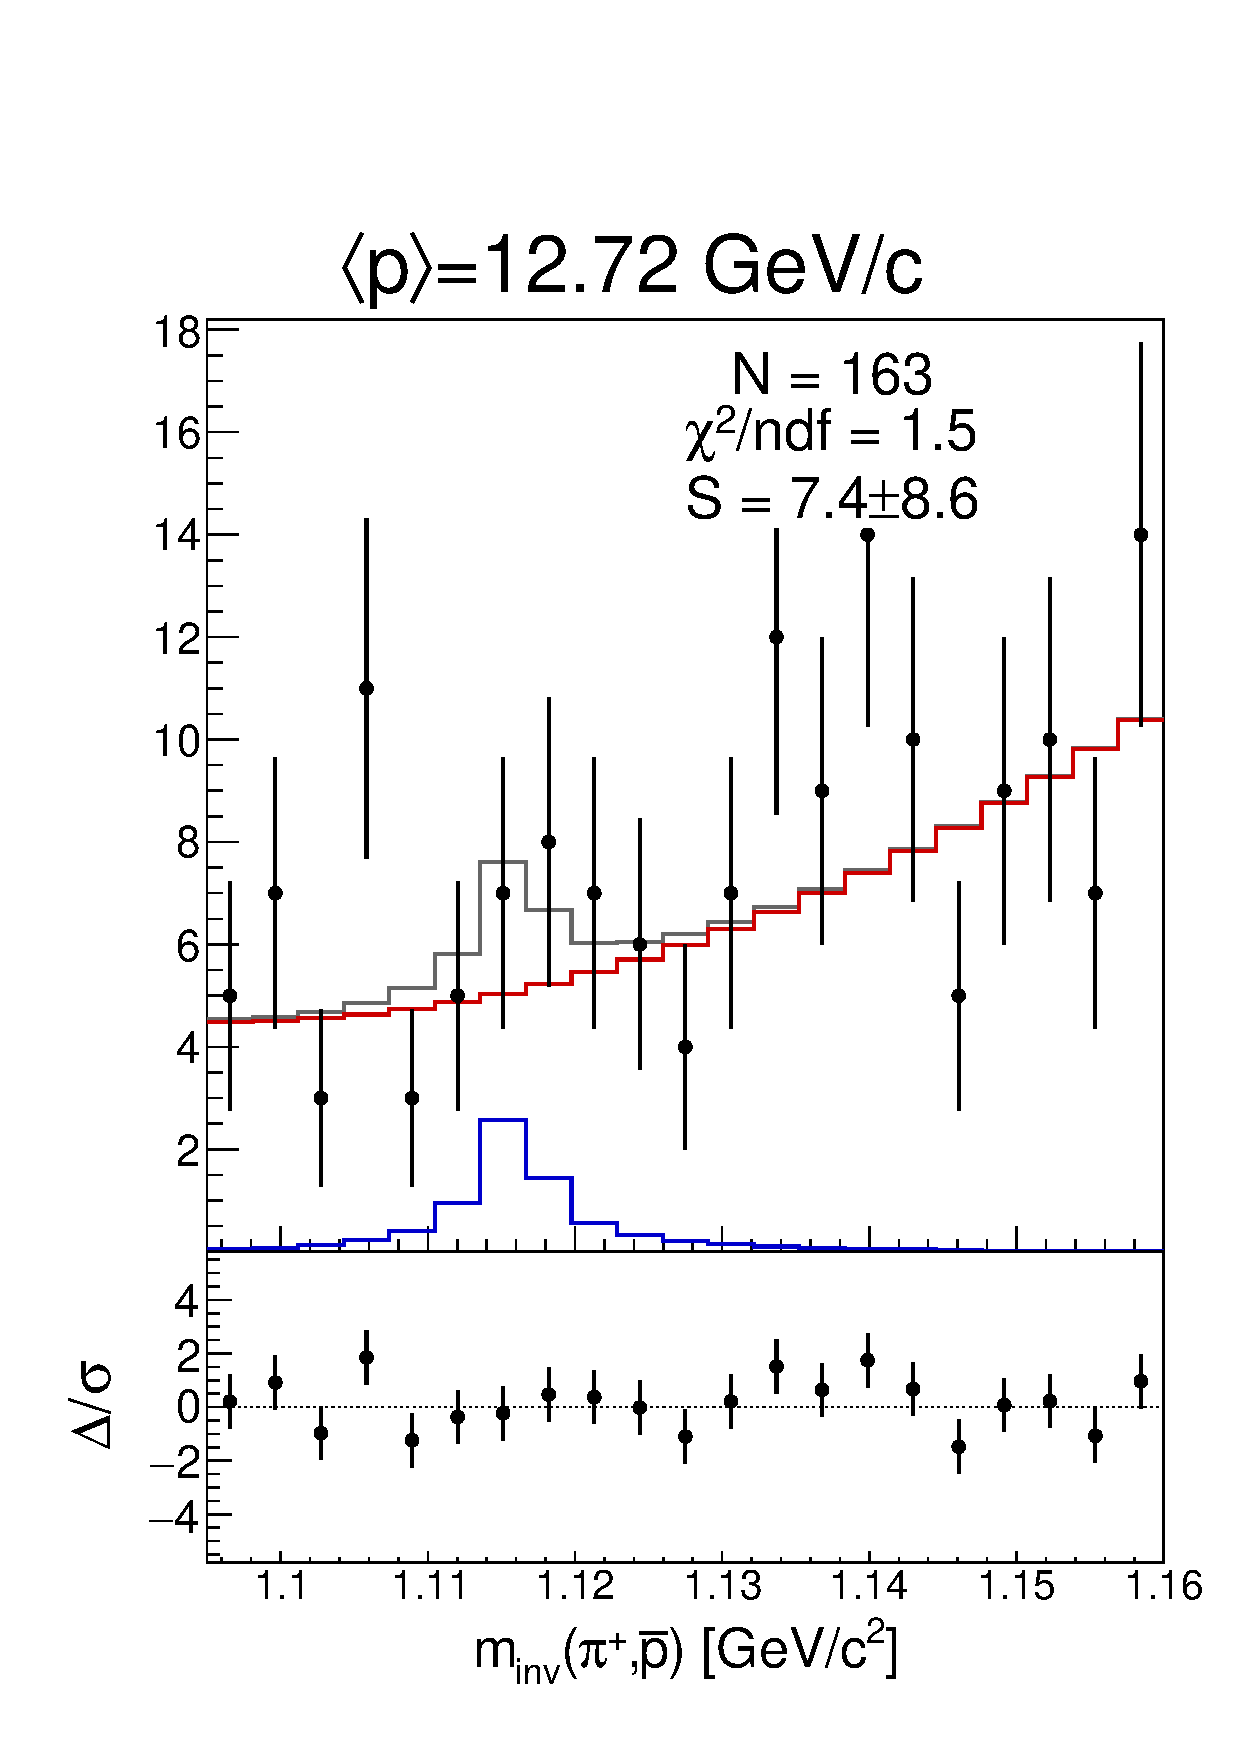
\includegraphics[clip, rviewport=0 0 1 1,width=0.32\textwidth]{vzero/mass_Data350_t1_ph0_h1_x3_y0}
  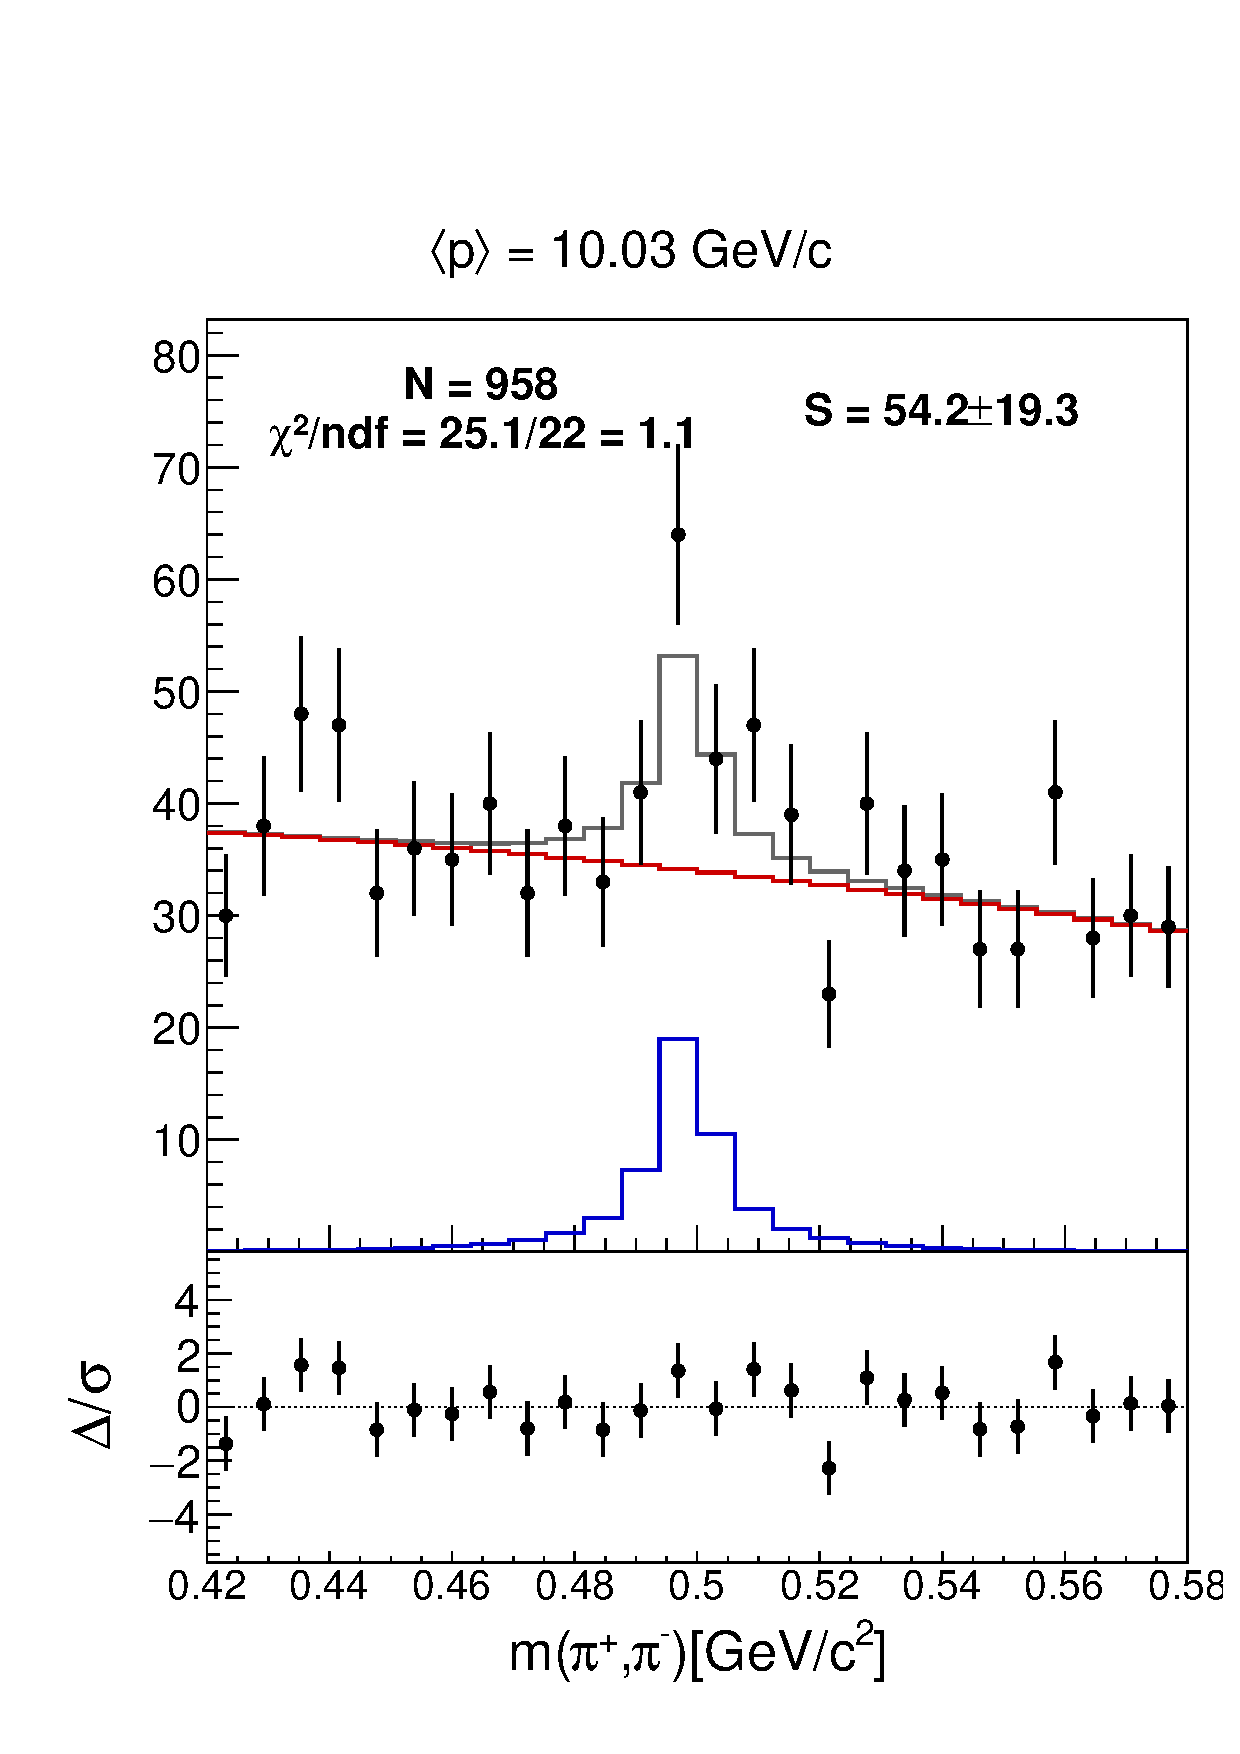
\includegraphics[clip, rviewport=0 0 1 1,width=0.32\textwidth]{vzero/mass_Data350_t1_ph0_h2_x3_y0}
  
  \caption{Examples of the fitted \minv distributions for the 350 \GeVc dataset, with target removed. The plot on left, middle and right shows \lamb, \antilamb and \kzeros, respectively.}
  \label{fig:hadron:vzero:signal:dist:350:out}
\end{figure}


%%%%%%%%%% BETA %%%%%%%%%%%%%%
\begin{figure}
  \centering
  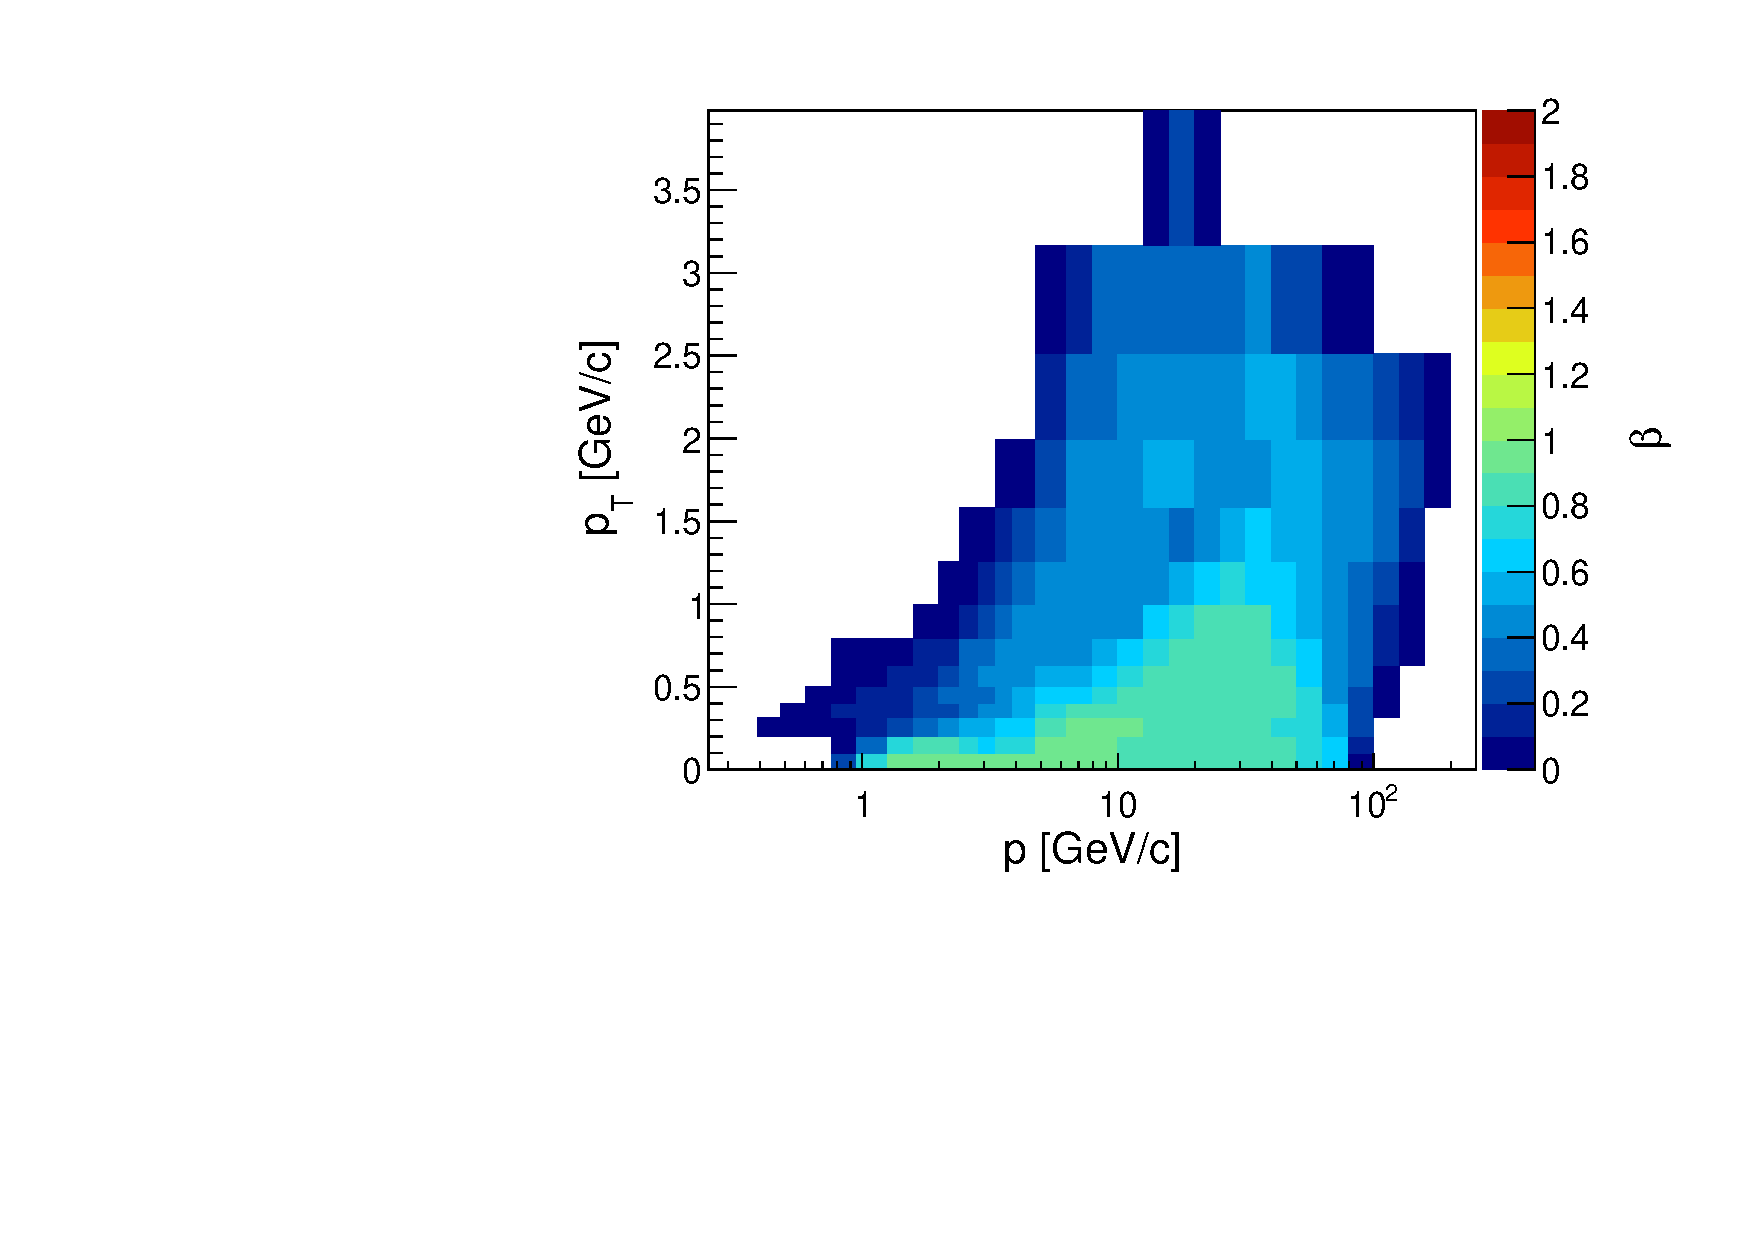
\includegraphics[clip, rviewport=0 0.13 1 0.94,width=0.4\textwidth]{dedx/fac_350_All_beta_c0_p1}
  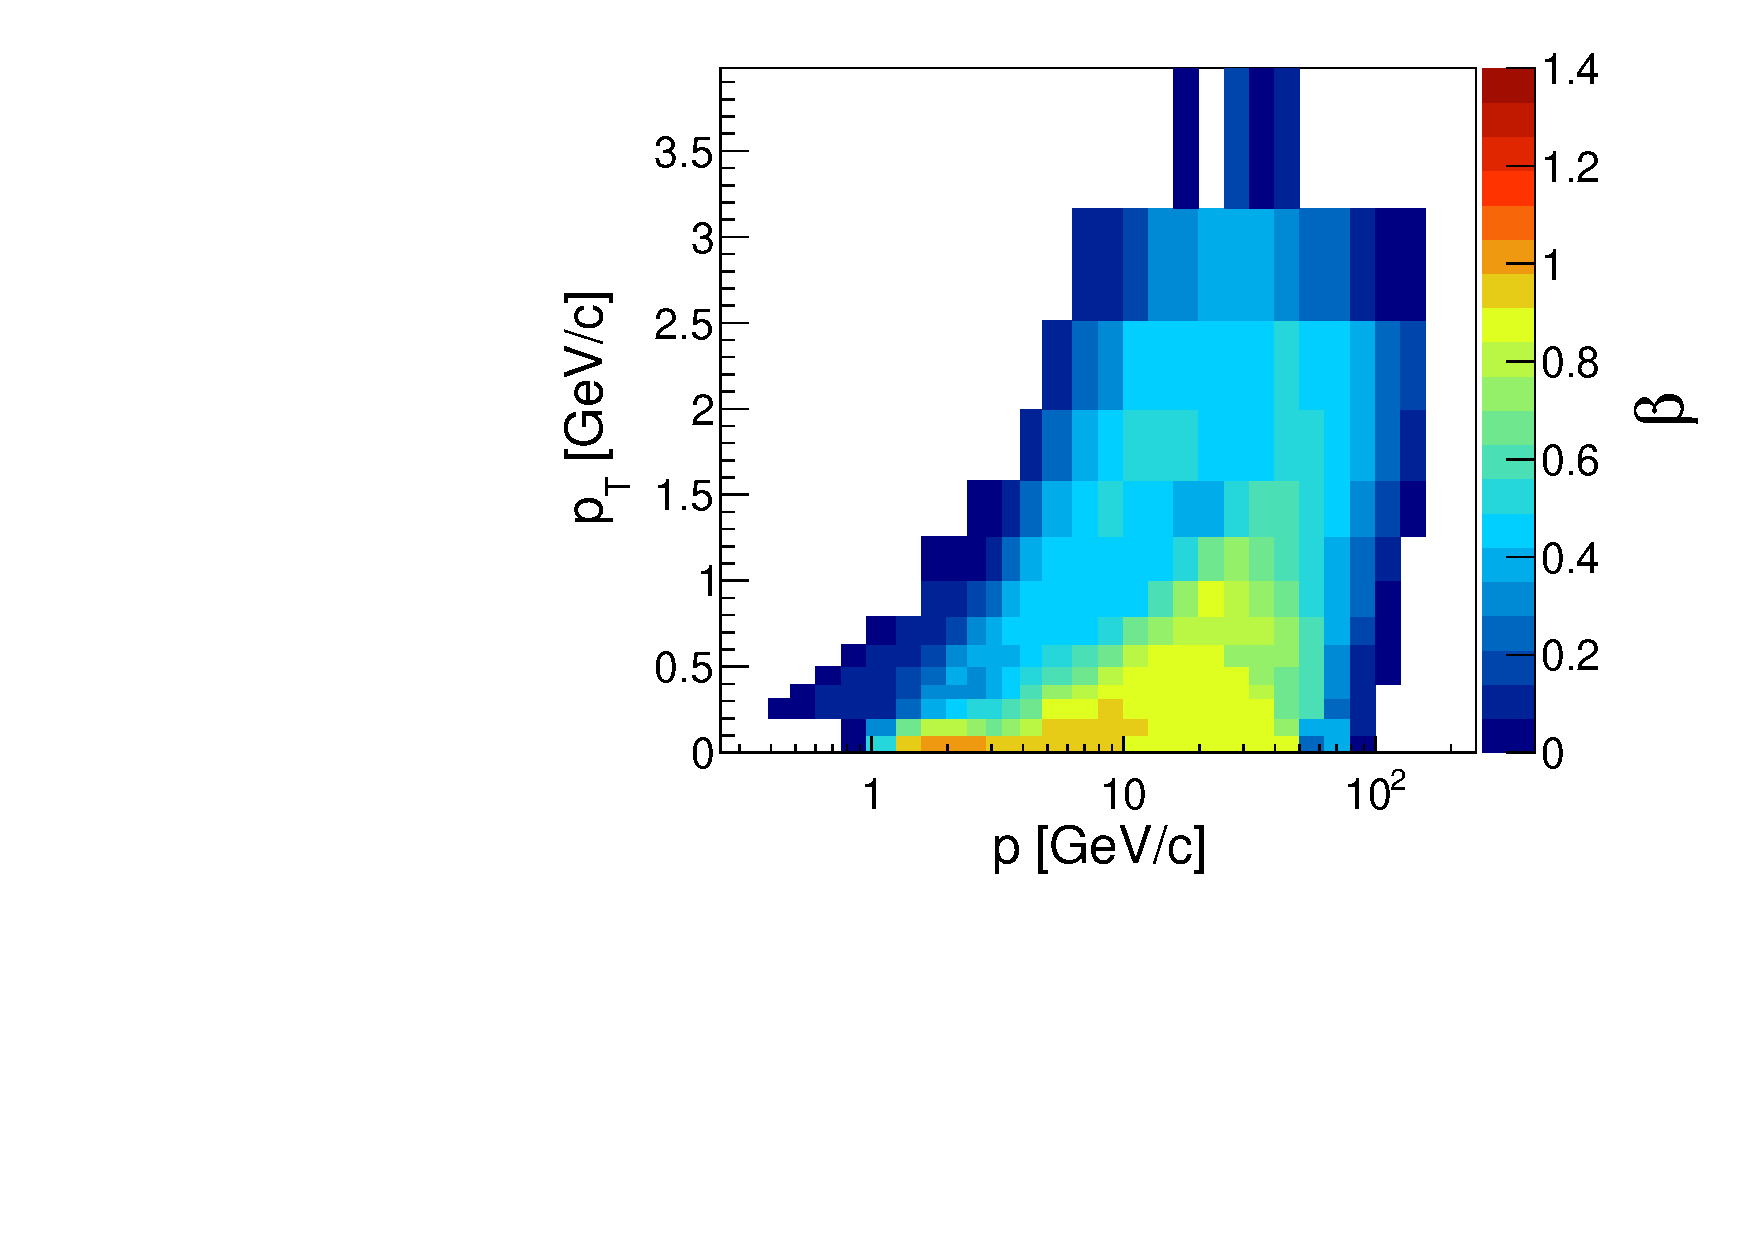
\includegraphics[clip, rviewport=0 0.13 1 0.94,width=0.4\textwidth]{dedx/fac_350_All_beta_c1_p1}

  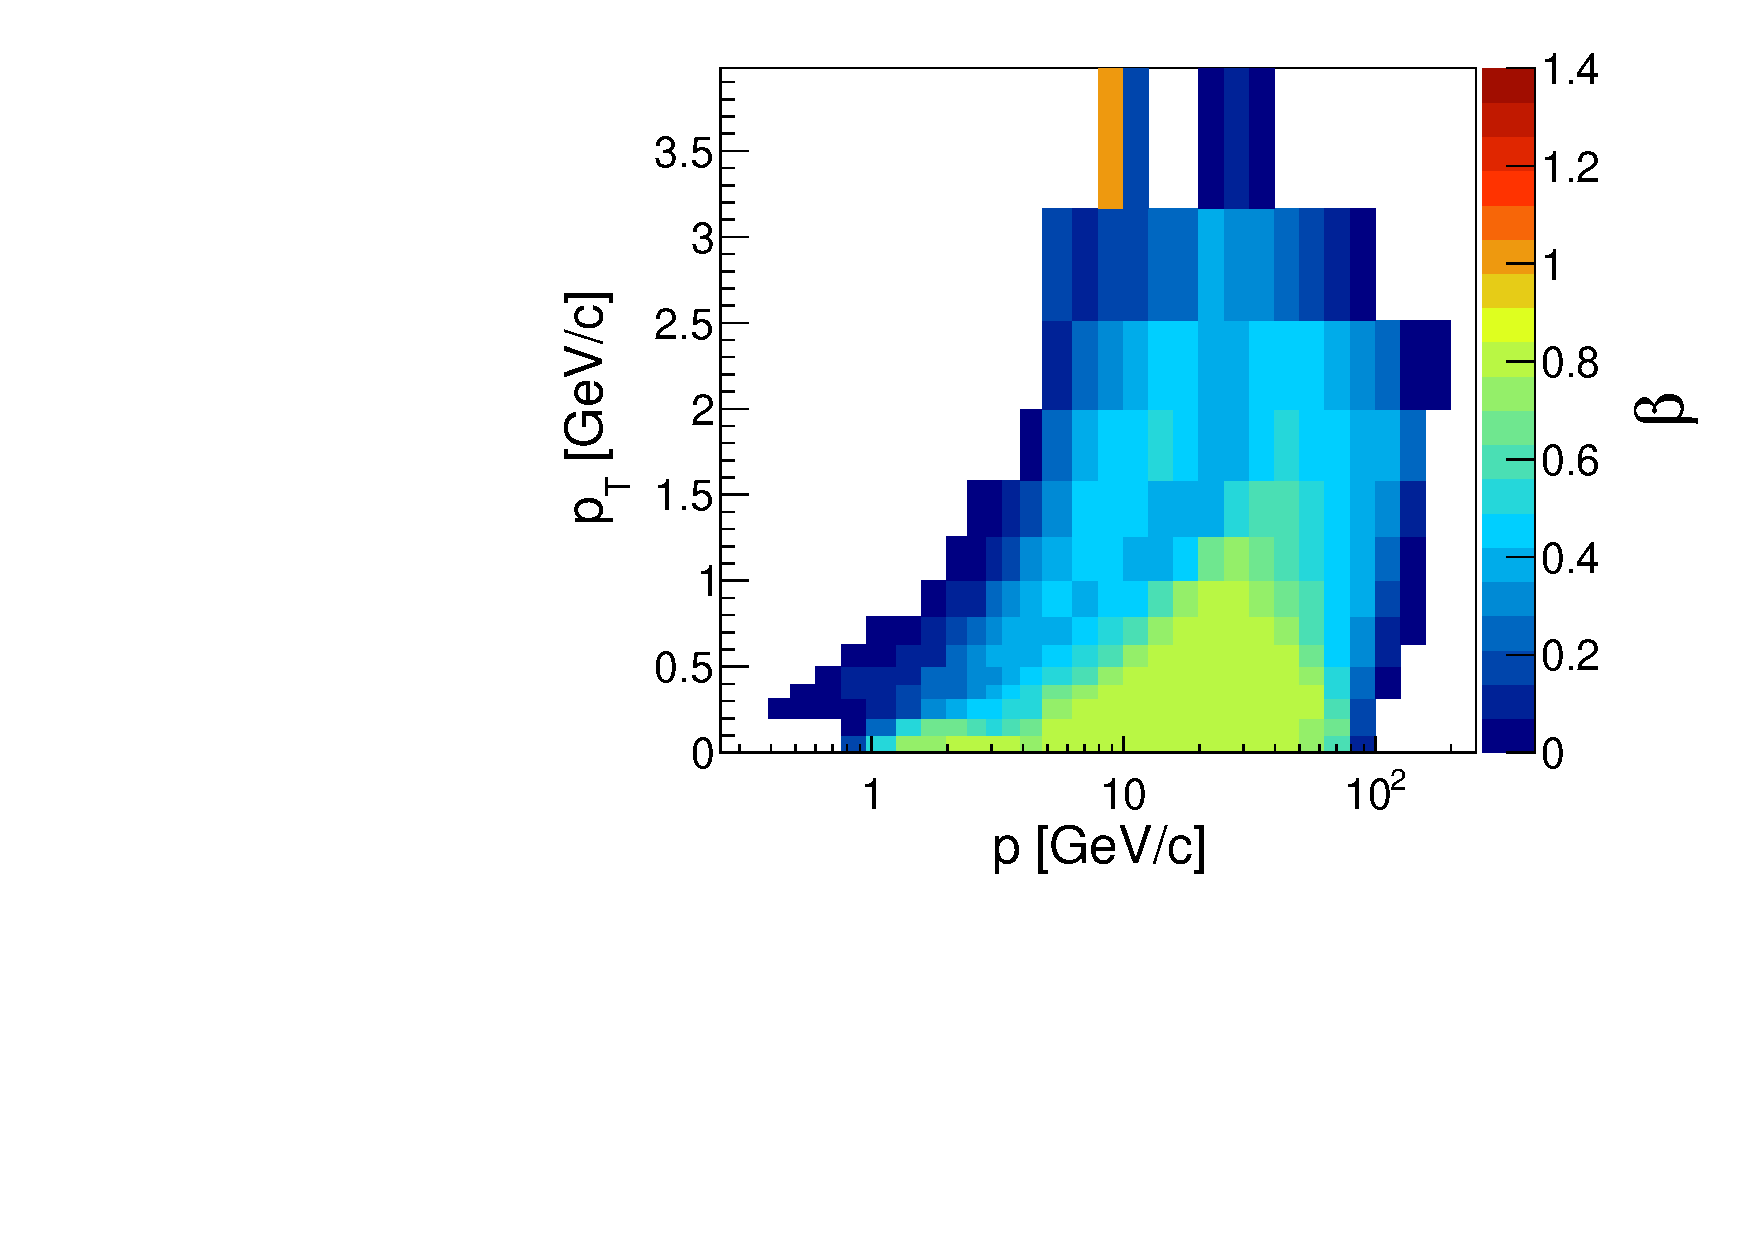
\includegraphics[clip, rviewport=0 0.13 1 0.94,width=0.4\textwidth]{dedx/fac_350_All_beta_c0_p2}
  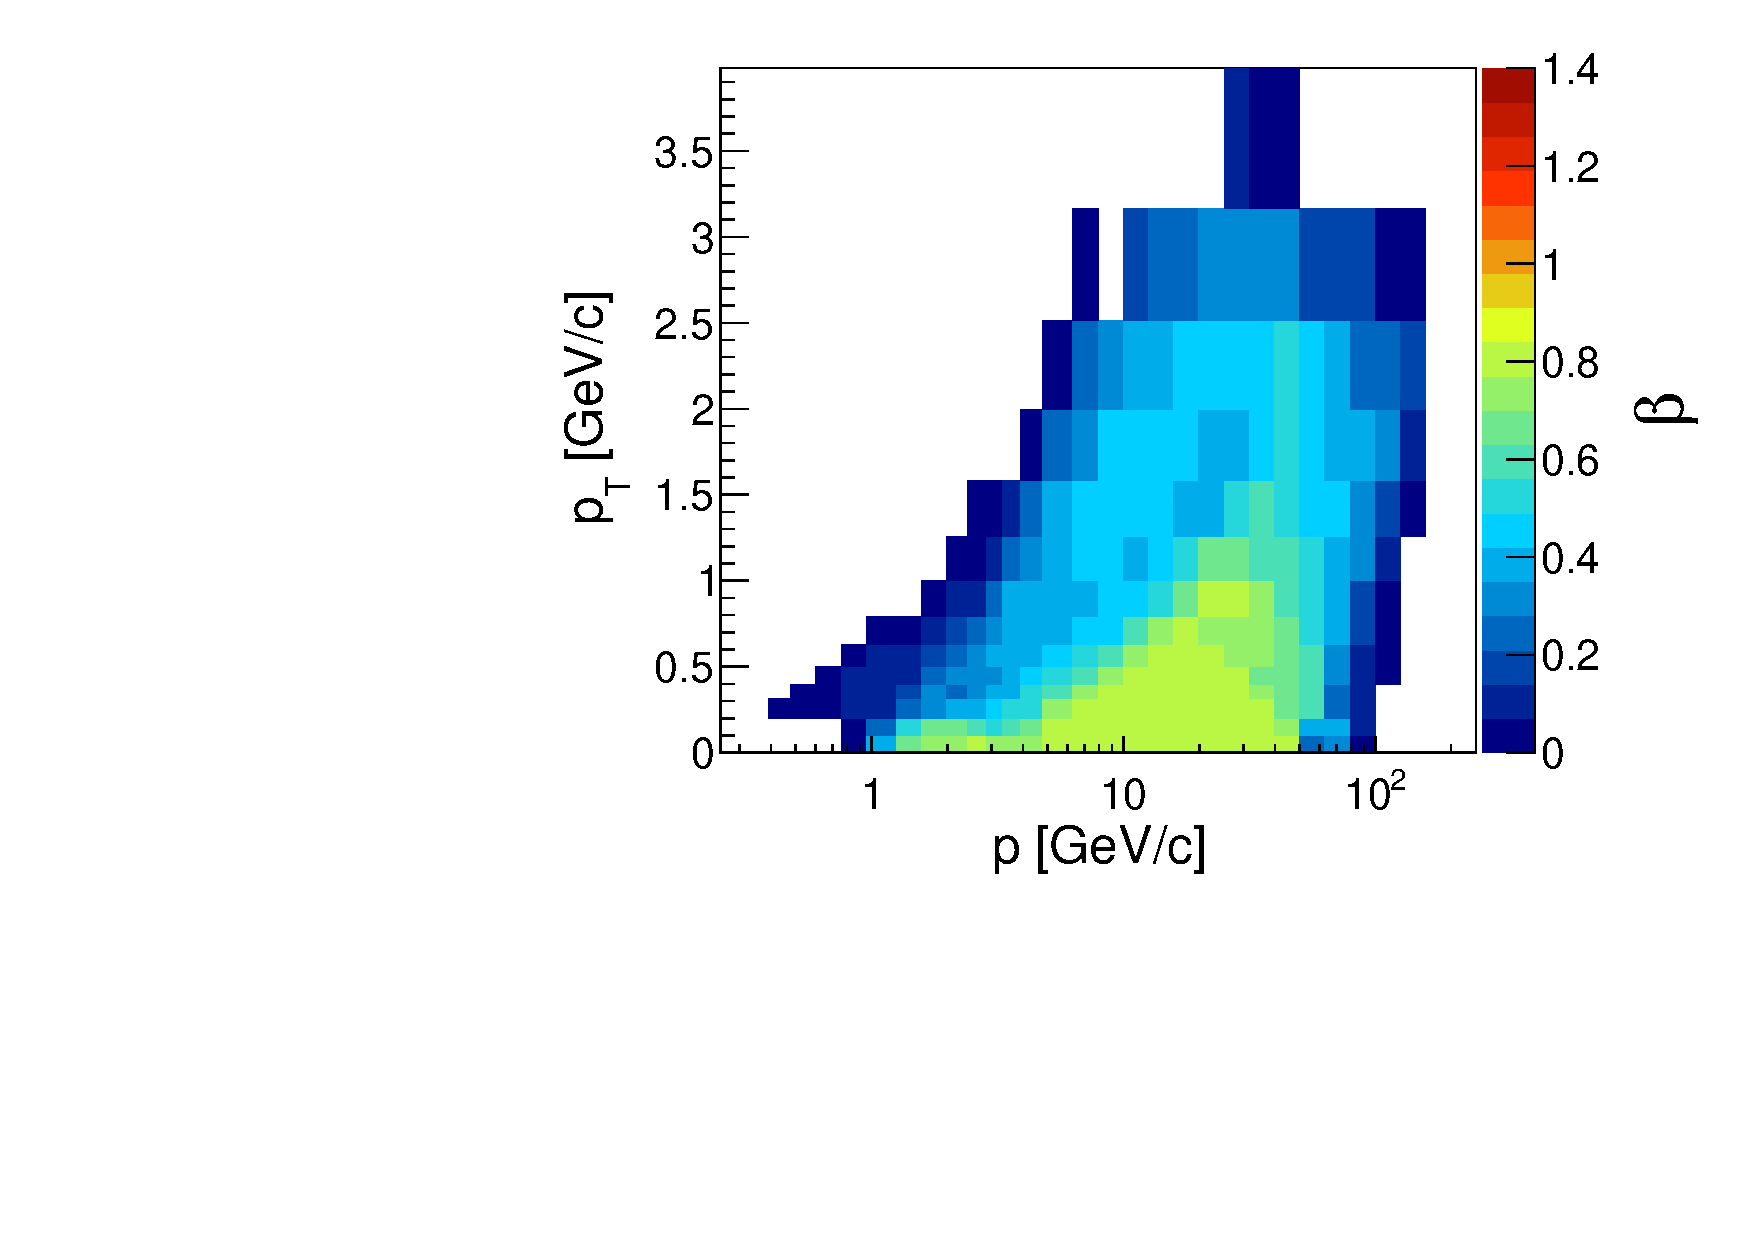
\includegraphics[clip, rviewport=0 0.13 1 0.94,width=0.4\textwidth]{dedx/fac_350_All_beta_c1_p2}

  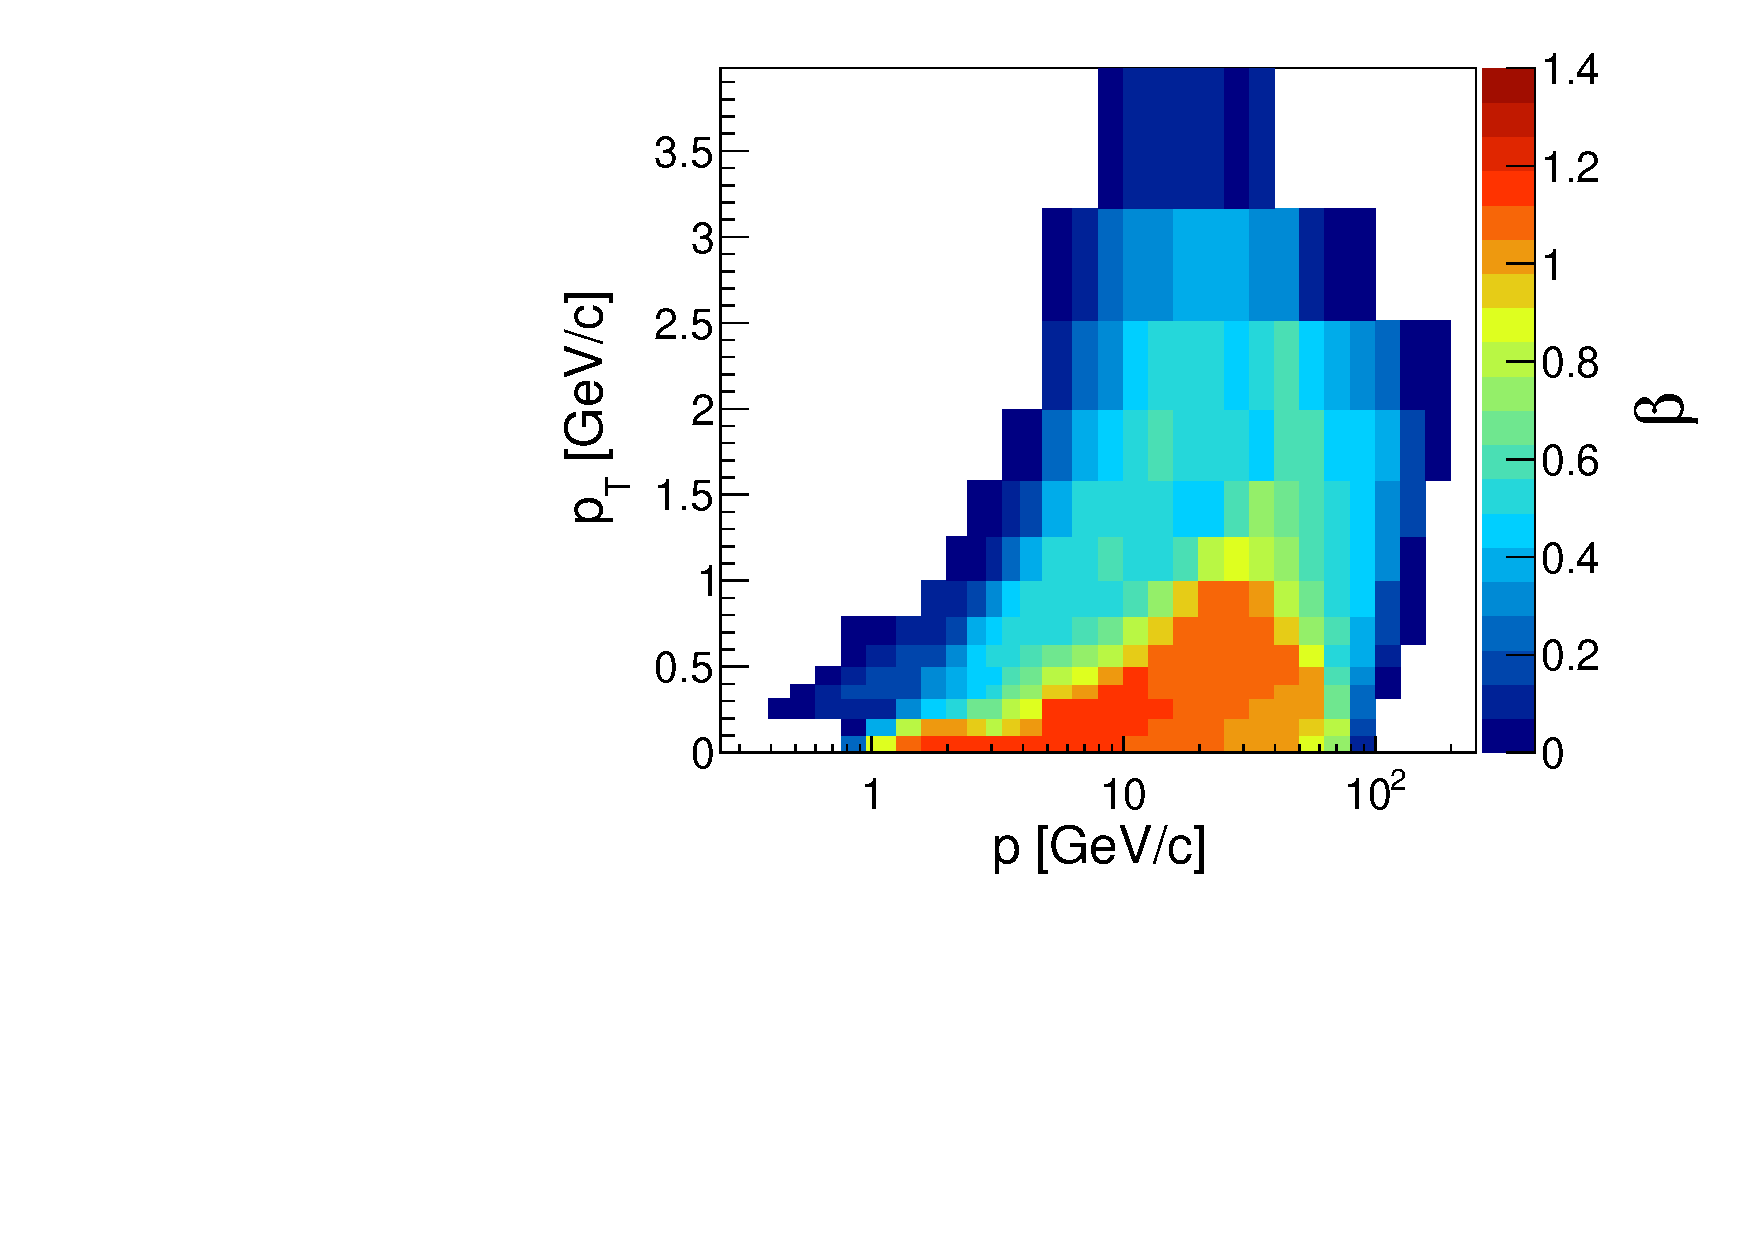
\includegraphics[clip, rviewport=0 0.13 1 0.94,width=0.4\textwidth]{dedx/fac_350_All_beta_c0_p3}
  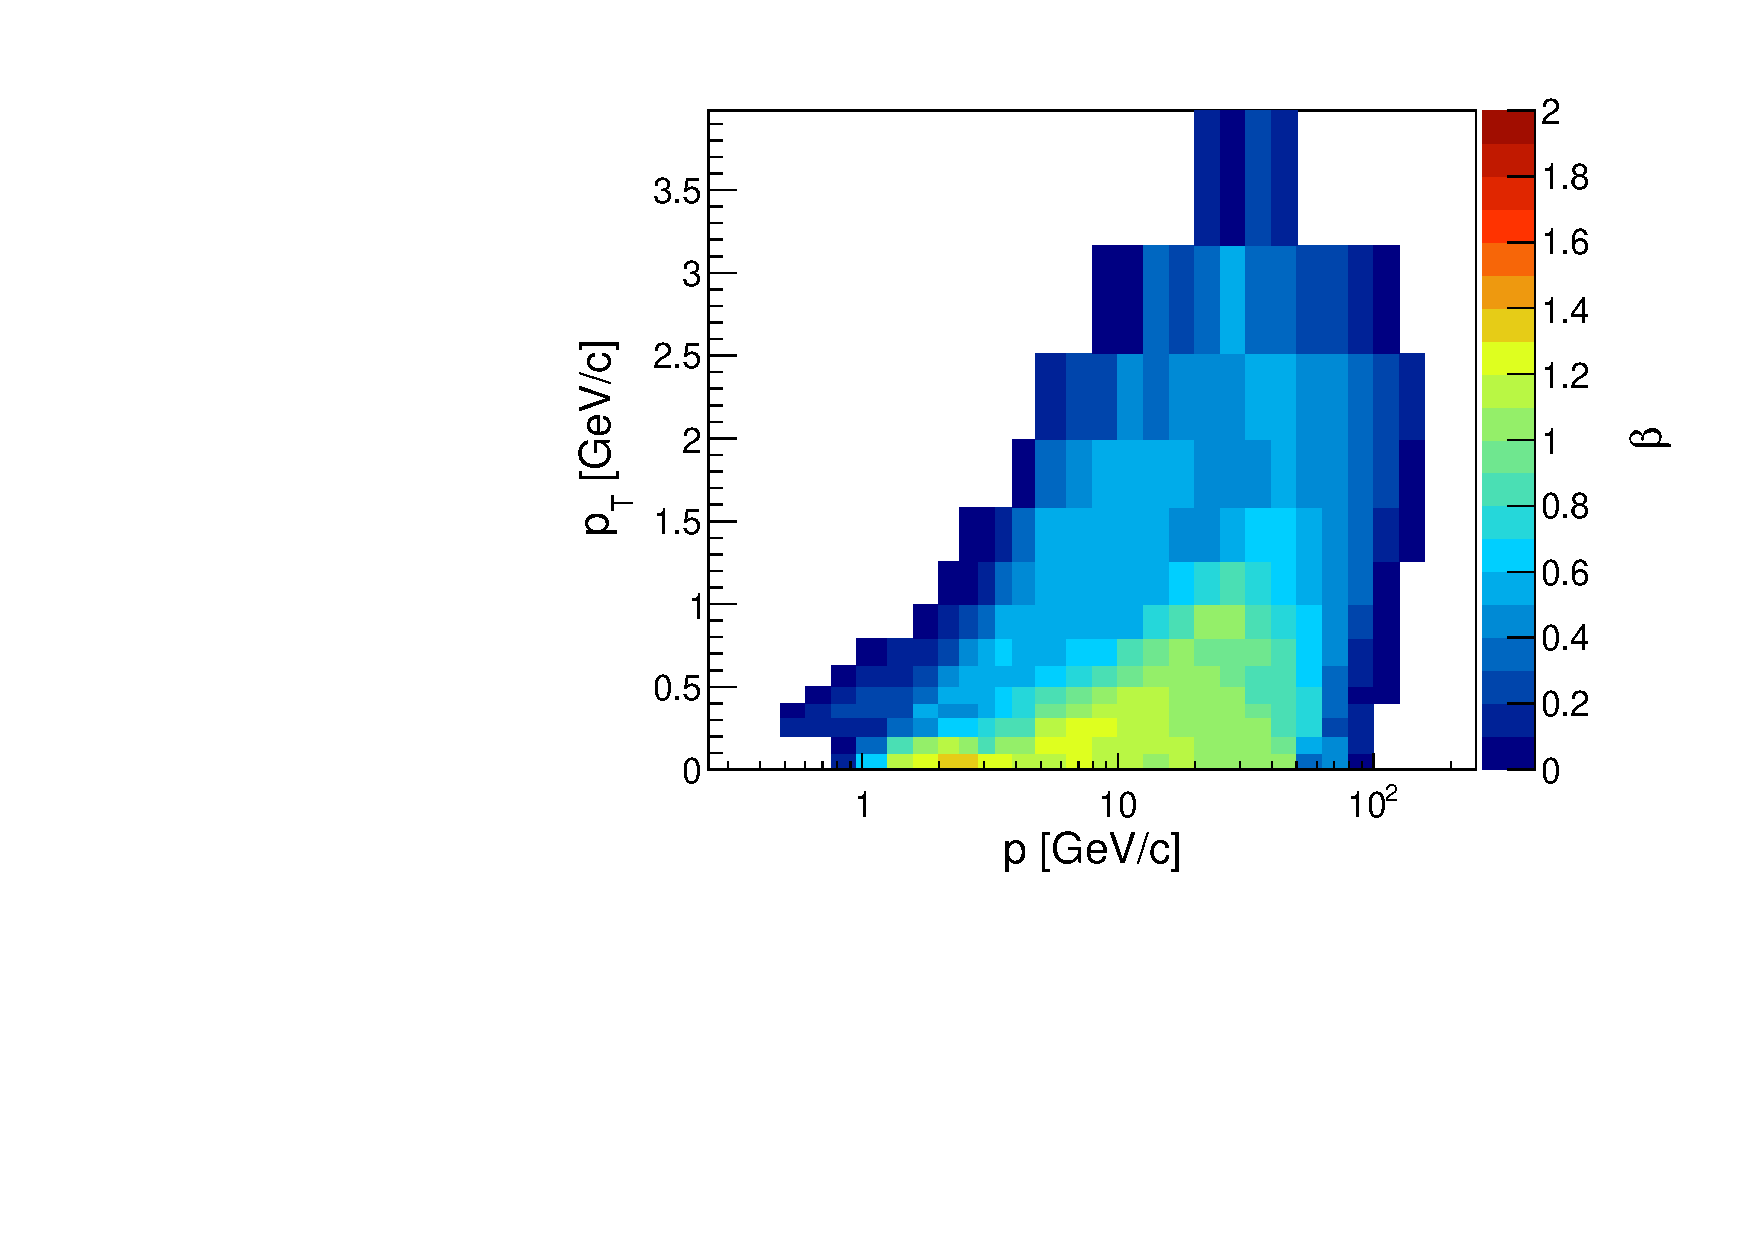
\includegraphics[clip, rviewport=0 0.13 1 0.94,width=0.4\textwidth]{dedx/fac_350_All_beta_c1_p3}

  \caption{$\beta$ correction factor for the 350 \GeVc dataset.}
  \label{fig:hadron:correction:beta:dedx350}
\end{figure}


%%%%%%%%%%% BETA %%%%%%%%%%%%%%%%%%
\begin{figure}
  \centering
  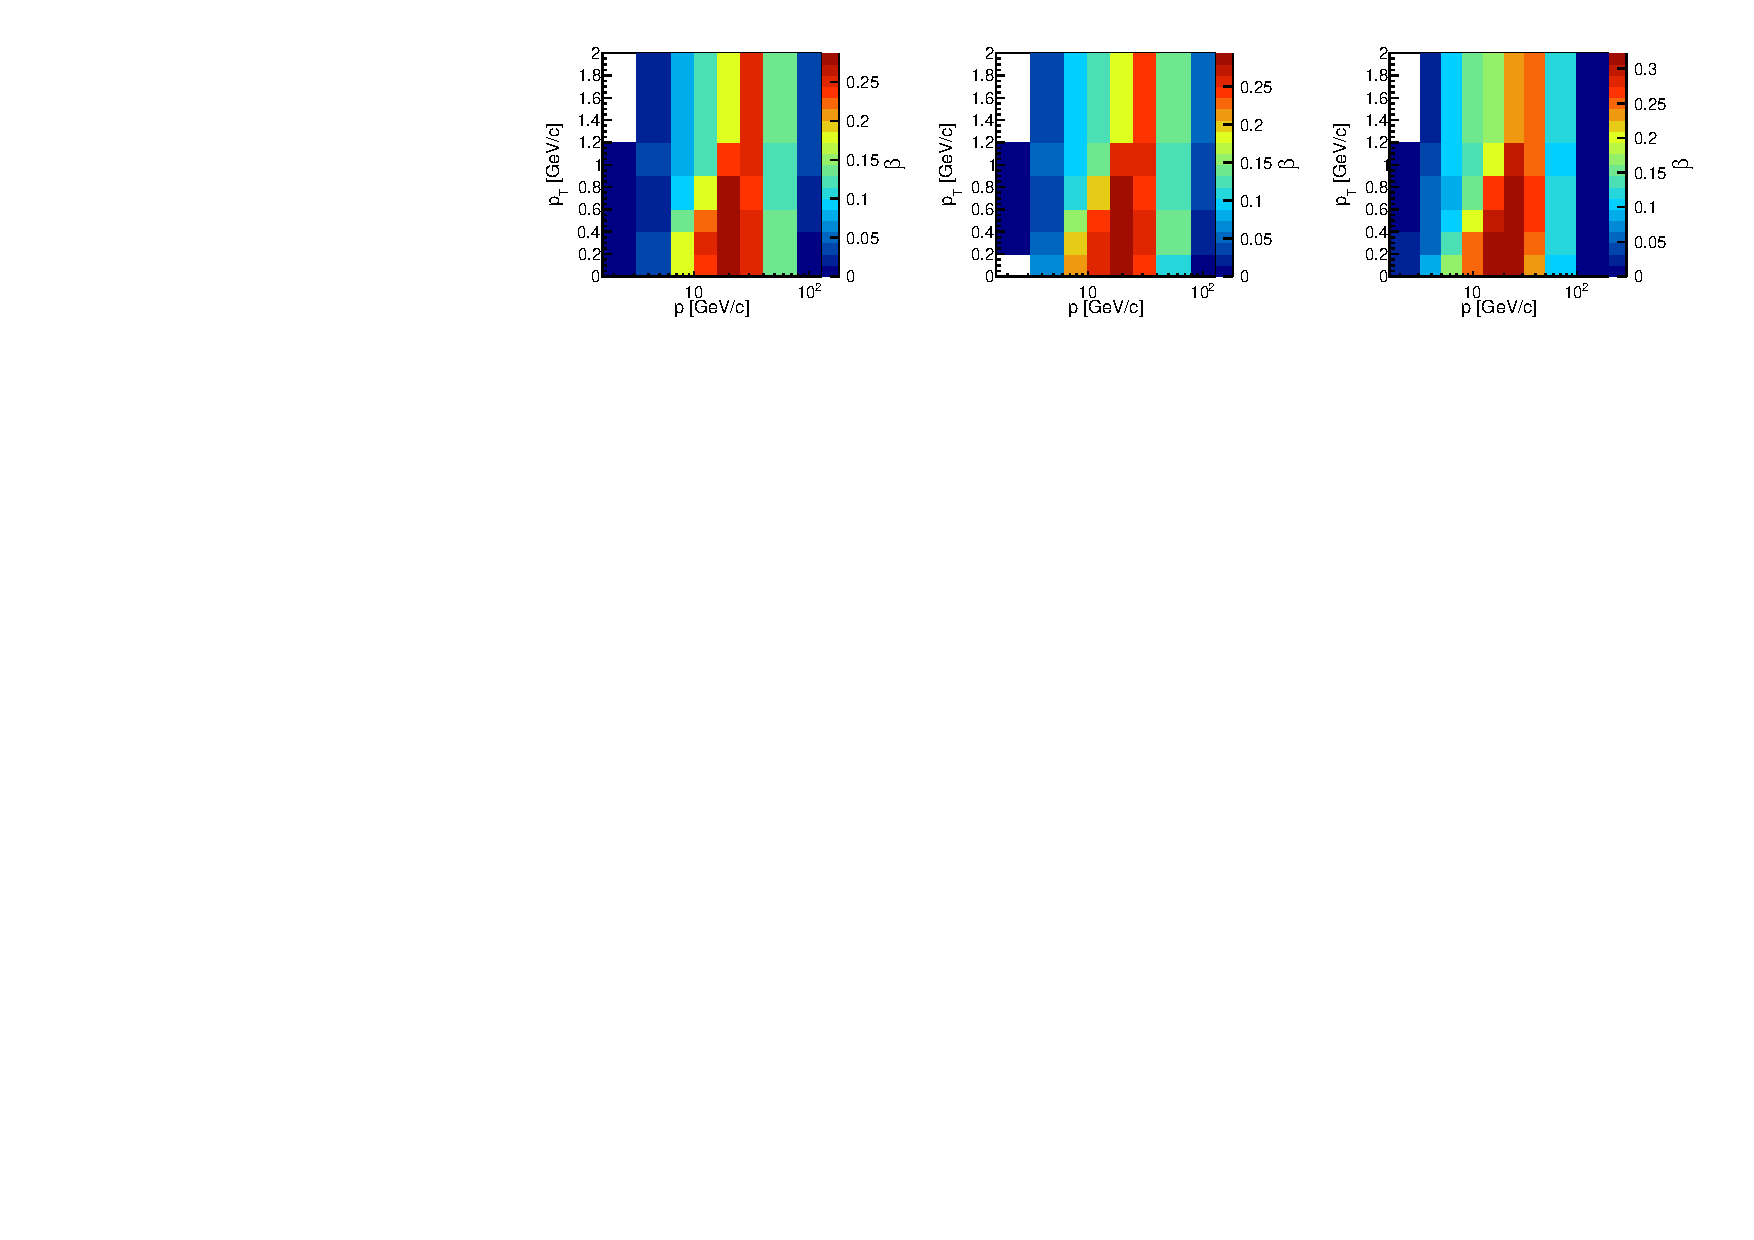
\includegraphics[clip, rviewport=0 0 1 1,width=0.95\textwidth]{vzero/beta350}
  
  \caption{$\beta$ correction factor for the 350 \GeVc dataset.}
  \label{fig:hadron:correction:beta:vzero350}
\end{figure}

